\documentclass[11pt]{report}

\usepackage[utf8]{inputenc}
\usepackage[super]{nth}
\usepackage{graphicx}
\usepackage{comment}
\usepackage[bookmarks]{hyperref}
\usepackage{textcomp}

\usepackage{titlesec}
\titleformat{\chapter}[display]   
{\normalfont\huge\bfseries}{\chaptertitlename\ \thechapter}{20pt}{\Huge}   
\titlespacing*{\chapter}{0pt}{-50pt}{40pt}
\titleformat{\chapter}[display]
  {\normalfont\huge\bfseries}{}{0pt}{\Huge}
\titlespacing*{\chapter}
  {0pt}{-50pt}{40pt}
  
\begin{document}

\begin{center}
\vspace*{\fill}
This document presents historical events known to mankind and occasionally provides a reference to a documentary or movie describing the event.\\
\vspace{5mm}
It is recommended that you use a PDF reader that displays the index for easier browsing.\\
\vspace{1cm}
By Virtuosek.\\ \vspace{5cm}
\end{center}

\vspace*{\fill}
\thispagestyle{empty}
\clearpage
\setcounter{page}{1}

\part{Billions of years ago}
\chapter{13.6 Billion years ago}
\section{Formation of the Milky Way}
\vspace{2mm}\begin{center}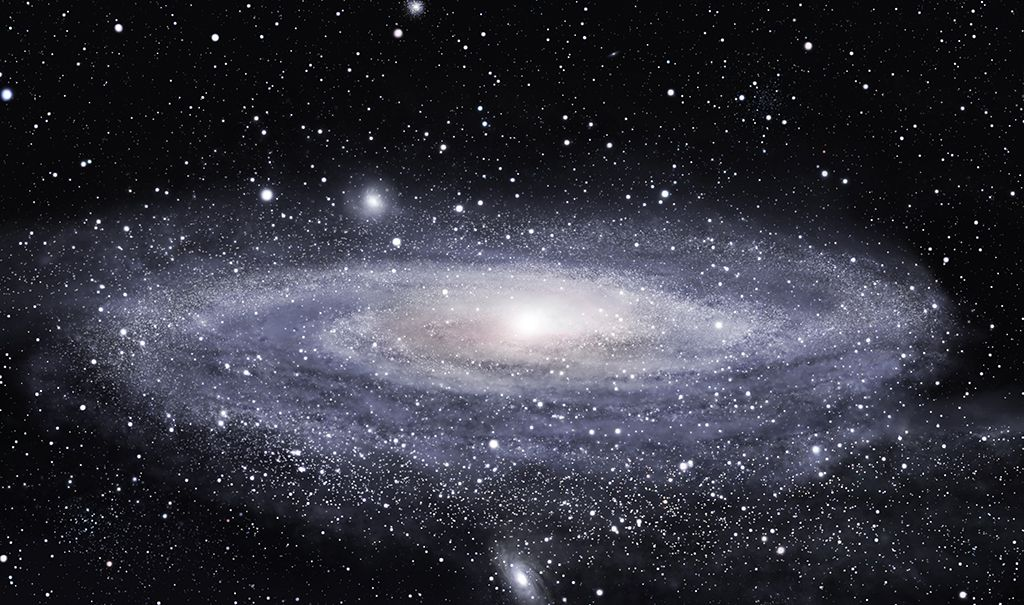
\includegraphics[width=4cm]{./img/milkyway.jpg}\end{center}
The Milky Way began as one or several small overdensities in the mass distribution in the Universe shortly after the Big Bang. Some of these overdensities were the seeds of globular clusters in which the oldest remaining stars in what is now the Milky Way formed. Nearly half the matter in the Milky Way may have come from other distant galaxies. Nonetheless, these stars and clusters now comprise the stellar halo of the Milky Way. Within a few billion years of the birth of the first stars, the mass of the Milky Way was large enough so that it was spinning relatively quickly. Due to conservation of angular momentum, this led the gaseous interstellar medium to collapse from a roughly spheroidal shape to a disk. Therefore, later generations of stars formed in this spiral disk. Most younger stars, including the Sun, are observed to be in the disk.\\
Since the first stars began to form, the Milky Way has grown through both galaxy mergers (particularly early in the Milky Way's growth) and accretion of gas directly from the Galactic halo. The Milky Way is currently accreting material from several small galaxies, including two of its largest satellite galaxies, the Large and Small Magellanic Clouds, through the Magellanic Stream. Direct accretion of gas is observed in high-velocity clouds like the Smith Cloud. However, properties of the Milky Way such as stellar mass, angular momentum, and metallicity in its outermost regions suggest it has undergone no mergers with large galaxies in the last 10 billion years. This lack of recent major mergers is unusual among similar spiral galaxies; its neighbor the Andromeda Galaxy appears to have a more typical history shaped by more recent mergers with relatively large galaxies.\\

\chapter{4.54 Billion years ago}
\section{Formation of planet Earth}
\vspace{2mm}\begin{center}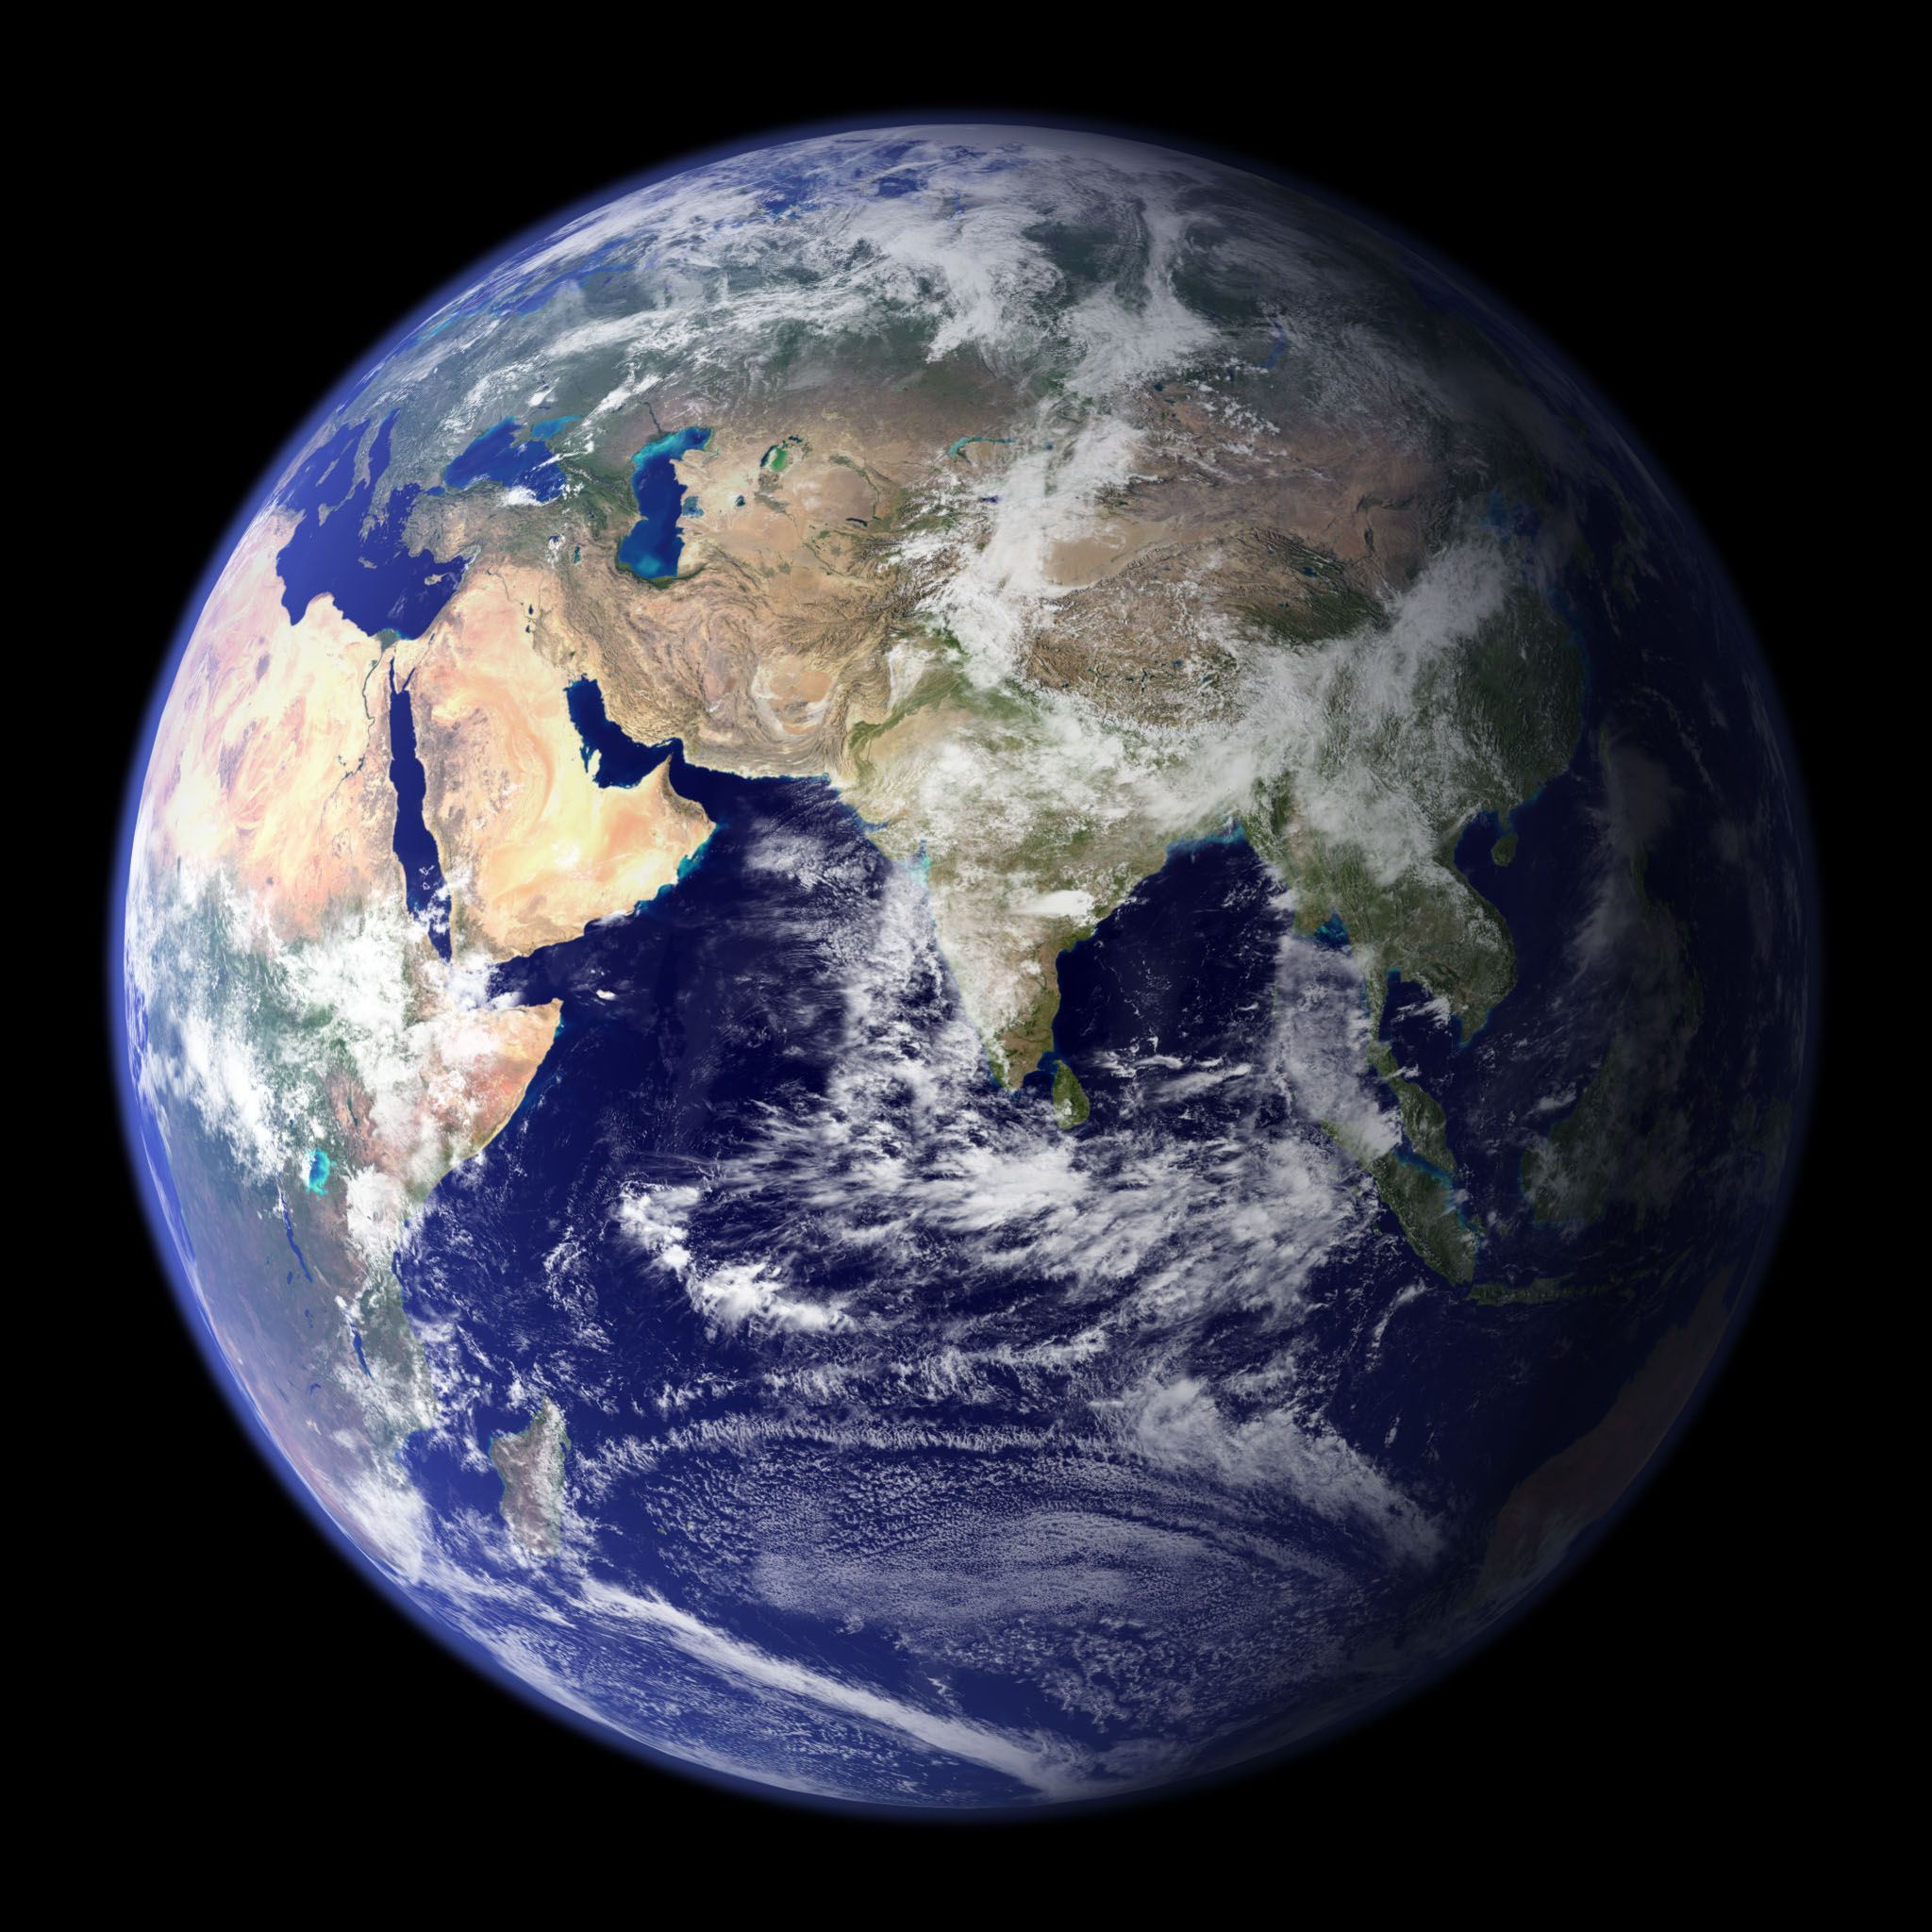
\includegraphics[width=6cm]{./img/earth.jpg}\end{center}
The history of Earth concerns the development of planet Earth from its formation to the present day. Nearly all branches of natural science have contributed to understanding of the main events of Earth's past, characterized by constant geological change and biological evolution.\\
The geological time scale (GTS), as defined by international convention, depicts the large spans of time from the beginning of the Earth to the present, and its divisions chronicle some definitive events of Earth history. (In the graphic: Ga means "billion years ago"; Ma, "million years ago".) Earth formed around 4.54 billion years ago, approximately one-third the age of the universe, by accretion from the solar nebula. Volcanic outgassing probably created the primordial atmosphere and then the ocean, but the early atmosphere contained almost no oxygen. Much of the Earth was molten because of frequent collisions with other bodies which led to extreme volcanism. While Earth was in its earliest stage (Early Earth), a giant impact collision with a planet-sized body named Theia is thought to have formed the Moon. Over time, the Earth cooled, causing the formation of a solid crust, and allowing liquid water on the surface.

\chapter{4.5 Billion years ago}
\section{Formation of The Moon}
\vspace{2mm}\begin{center}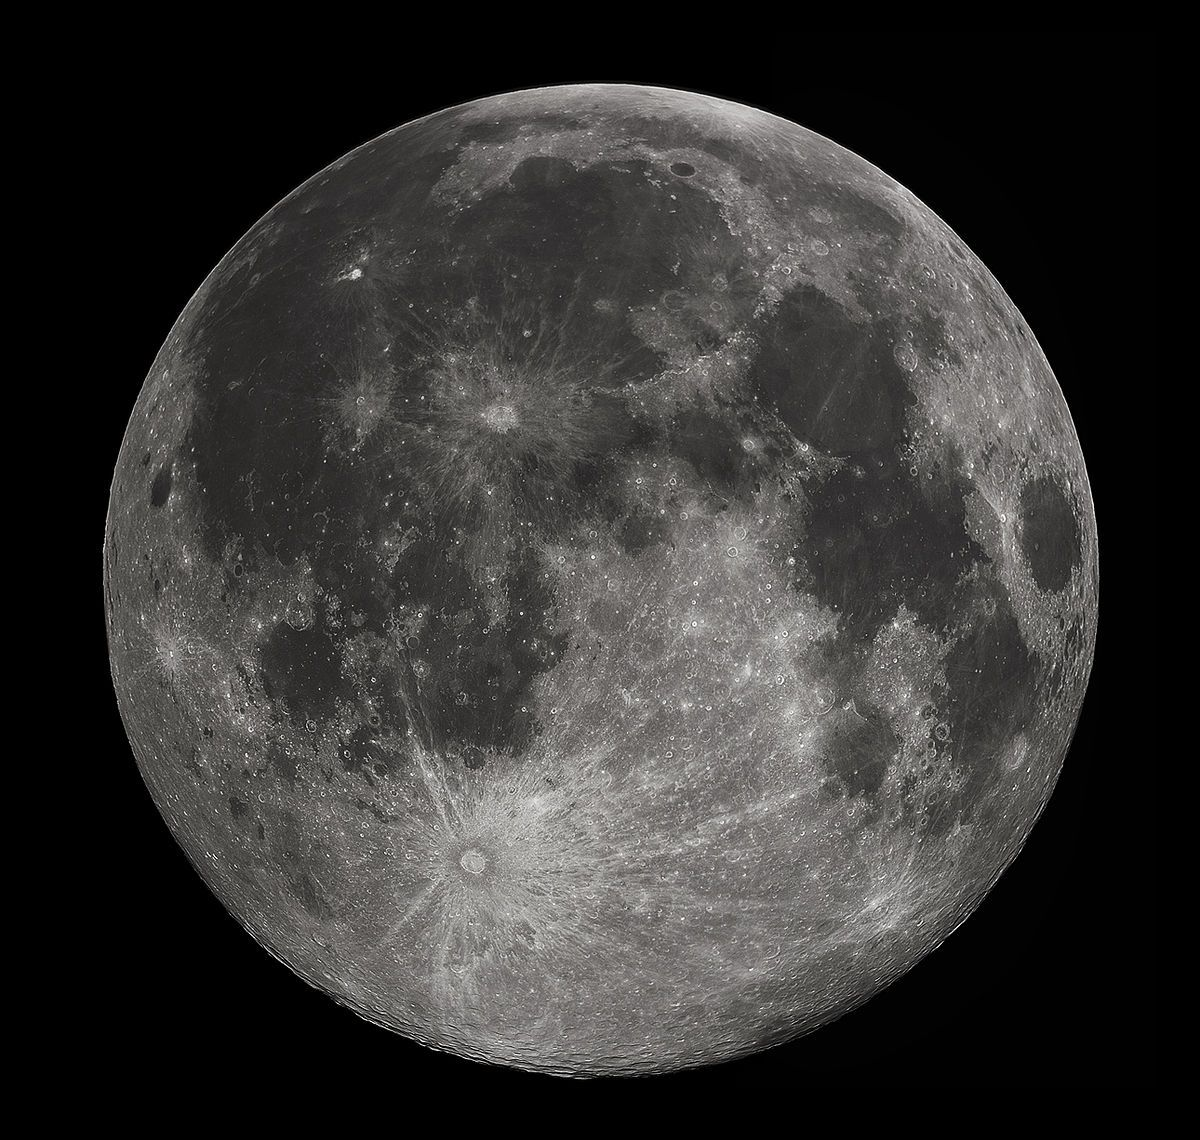
\includegraphics[width=8cm]{./img/moon.jpg}\end{center}
\textbf{Giant-impact hypothesis}:\\
The giant-impact hypothesis, sometimes called the Big Splash, or the Theia Impact suggests that the Moon formed out of the debris left over from a collision between Earth and an astronomical body the size of Mars, approximately 4.5 billion years ago, in the Hadean eon; about 20 to 100 million years after the solar system coalesced. The colliding body is sometimes called Theia, from the name of the mythical Greek Titan who was the mother of Selene, the goddess of the Moon. Analysis of lunar rocks, published in a 2016 report, suggests that the impact may have been a direct hit, causing a thorough mixing of both parent bodies.

\chapter{1.6 Billion years ago}
\section{Appearance of Eukaryotic cells}
\vspace{2mm}\begin{center}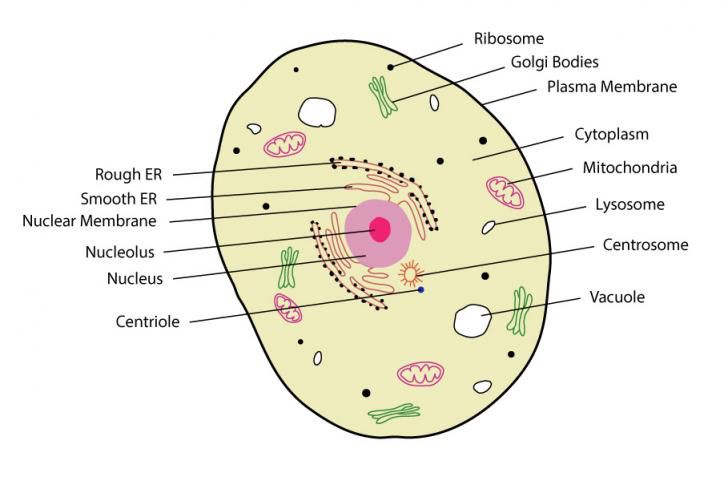
\includegraphics[width=6cm]{./img/eukaryoticCell.jpg}\end{center}
Eukaryotes are organisms whose cells have a nucleus enclosed within membranes, unlike prokaryotes (Bacteria and Archaea). Eukaryotic cells also contain other membrane-bound organelles such as mitochondria and the Golgi apparatus, and in addition, some cells of plants and algae contain chloroplasts. Unlike unicellular archaea and bacteria, eukaryotes may also be multicellular and include organisms consisting of many cell types forming different kinds of tissue. Animals and plants are the most familiar eukaryotes.\\
Eukaryotes can reproduce both asexually through mitosis and sexually through meiosis and gamete fusion. In mitosis, one cell divides to produce two genetically identical cells. In meiosis, DNA replication is followed by two rounds of cell division to produce four haploid daughter cells. These act as sex cells (gametes). Each gamete has just one set of chromosomes, each a unique mix of the corresponding pair of parental chromosomes resulting from genetic recombination during meiosis.\\
The domain Eukaryota appears to be monophyletic, and makes up one of the domains of life in the three-domain system. The two other domains, Bacteria and Archaea, are prokaryotes and have none of the above features. Eukaryotes represent a tiny minority of all living things. However, due to their generally much larger size, their collective worldwide biomass is estimated to be about equal to that of prokaryotes. Eukaryotes evolved approximately 1.6–2.1 billion years ago, during the Proterozoic eon.

%             					2599-2500 bc

\part{2599-2500 BC}
\chapter{2560 BC}
\section{Building of the Great Pyramid of Giza}
\vspace{2mm}\begin{center}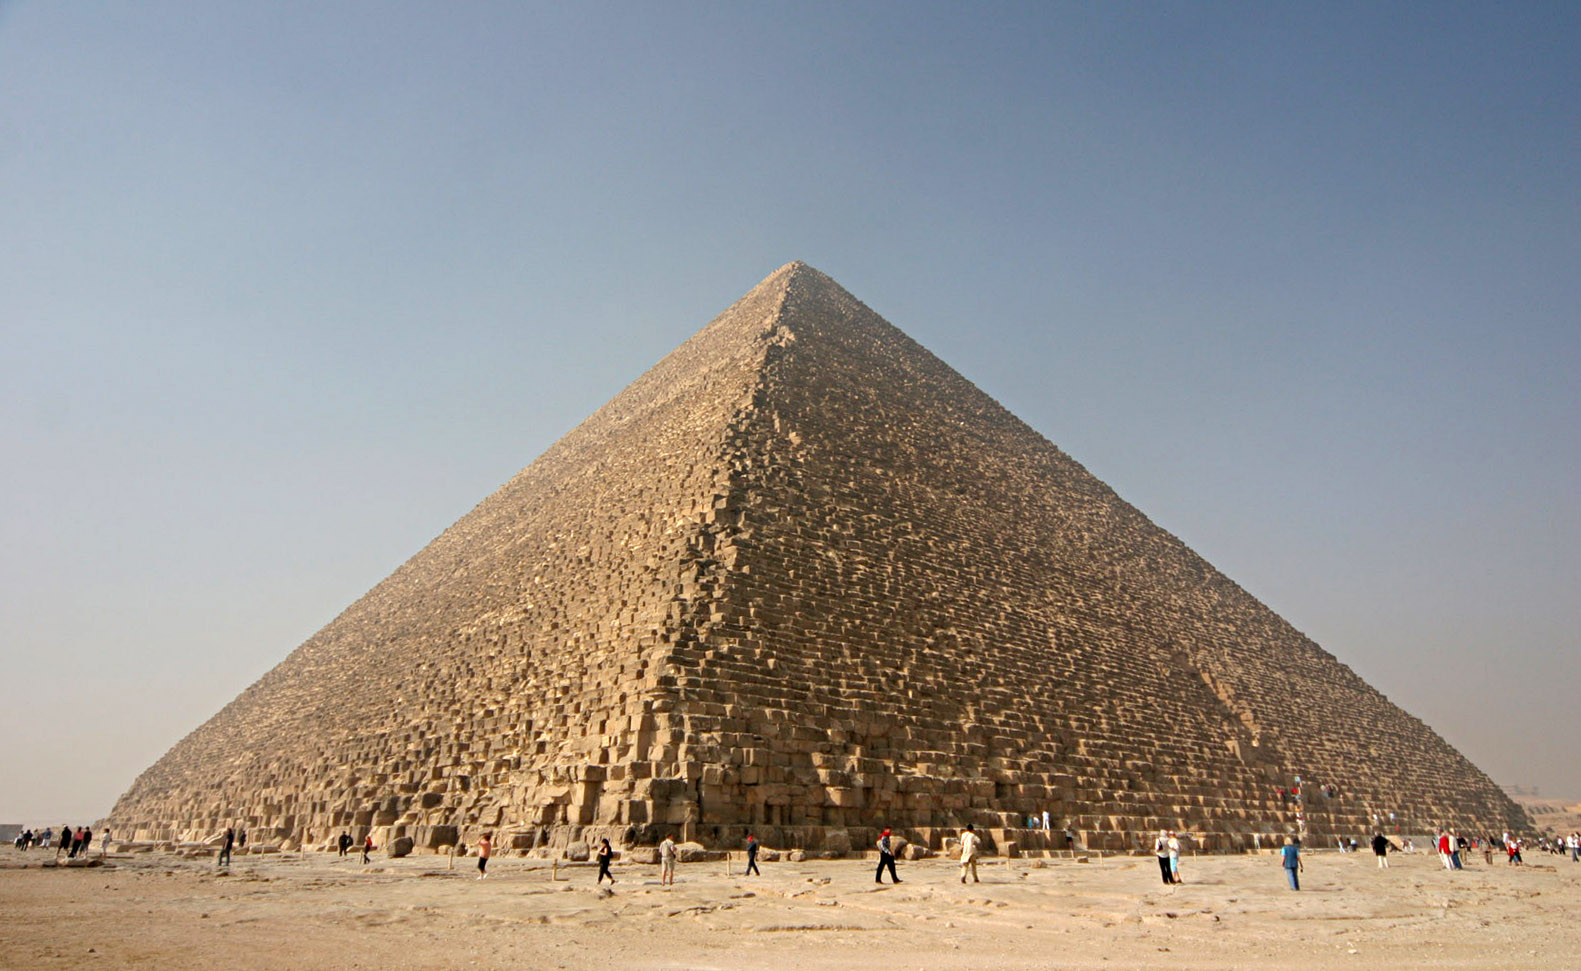
\includegraphics[width=8cm]{./img/greatPyrGiza.jpg}\end{center}
The Great Pyramid of Giza (also known as the Pyramid of Khufu or the Pyramid of Cheops) is the oldest and largest of the three pyramids in the Giza pyramid complex bordering what is now El Giza, Egypt. It is the oldest of the Seven Wonders of the Ancient World, and the only one to remain largely intact.\\
\indent Based on a mark in an interior chamber naming the work gang and a reference to the fourth dynasty Egyptian Pharaoh Khufu, Egyptologists believe that the pyramid was built as a tomb over a 10- to 20-year period concluding around 2560 BC. Initially at 146.5 metres (481 feet), the Great Pyramid was the tallest man-made structure in the world for more than 3,800 years. Originally, the Great Pyramid was covered by limestone casing stones that formed a smooth outer surface; what is seen today is the underlying core structure. Some of the casing stones that once covered the structure can still be seen around the base. There have been varying scientific and alternative theories about the Great Pyramid's construction techniques. Most accepted construction hypotheses are based on the idea that it was built by moving huge stones from a quarry and dragging and lifting them into place.

%             					499-400 bc

\part{499-400 BC}
\chapter{470 BC}
\subsection{Birth of Socrates}
\vspace{2mm}\begin{center}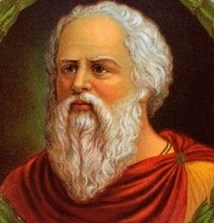
\includegraphics[width=5cm]{./img/socrates.jpg}\end{center}
The year of birth of Socrates stated is an assumed date, or estimate, given the fact of the dating of anything in ancient history in part being sometimes reliant on argument stemming from the inexact period floruit of individuals. Diogenes Laërtius stated Socrates birth date was "the sixth day of Thargelion, the day when the Athenians purify the city". Contemporaneous sources state, he was born not very much later than sometime after the year 471, his date of birth is within the period of years ranging 470 to 469 BC, or within a range 469 to 468 BC (corresponding to the fourth year of the 77th Olympiad).\\
Socrates was born in Alopeke, and belonged to the tribe Antiochis. His father was Sophroniscus, a sculptor, or stonemason. His mother was a midwife named Phaenarete. Socrates married Xanthippe, who is especially remembered for having an undesirable temperament. She bore for him three sons, Lamprocles, Sophroniscus and Menexenus.

%             					400-300 bc

\part{400-300 BC}
\chapter{356 BC}
\section{July 20/21}
\subsection{Birth of Alexander III of Macedon}
\vspace{2mm}\begin{center}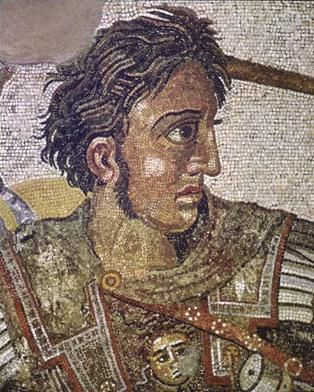
\includegraphics[width=3cm]{./img/alexanderTG.jpg}\end{center}
Alexander was born on the sixth day of the ancient Greek month of Hekatombaion, which probably corresponds to 20 July 356 BC, although the exact date is disputed, in Pella, the capital of the Kingdom of Macedon. He was the son of the king of Macedon, Philip II, and his fourth wife, Olympias, the daughter of Neoptolemus I, king of Epirus. Although Philip had seven or eight wives, Olympias was his principal wife for some time, likely because she gave birth to Alexander.\\
Statue of Alexander the Great in Thessaloniki, Macedonia, Greece
Several legends surround Alexander's birth and childhood. According to the ancient Greek biographer Plutarch, on the eve of the consummation of her marriage to Philip, Olympias dreamed that her womb was struck by a thunder bolt that caused a flame to spread "far and wide" before dying away. Sometime after the wedding, Philip is said to have seen himself, in a dream, securing his wife's womb with a seal engraved with a lion's image. Plutarch offered a variety of interpretations of these dreams: that Olympias was pregnant before her marriage, indicated by the sealing of her womb; or that Alexander's father was Zeus. Ancient commentators were divided about whether the ambitious Olympias promulgated the story of Alexander's divine parentage, variously claiming that she had told Alexander, or that she dismissed the suggestion as impious

%             					1st century

\part{1st century}
\chapter{80}
\section{-}
\subsection{Completion of the Colosseum}
\vspace{2mm}\begin{center}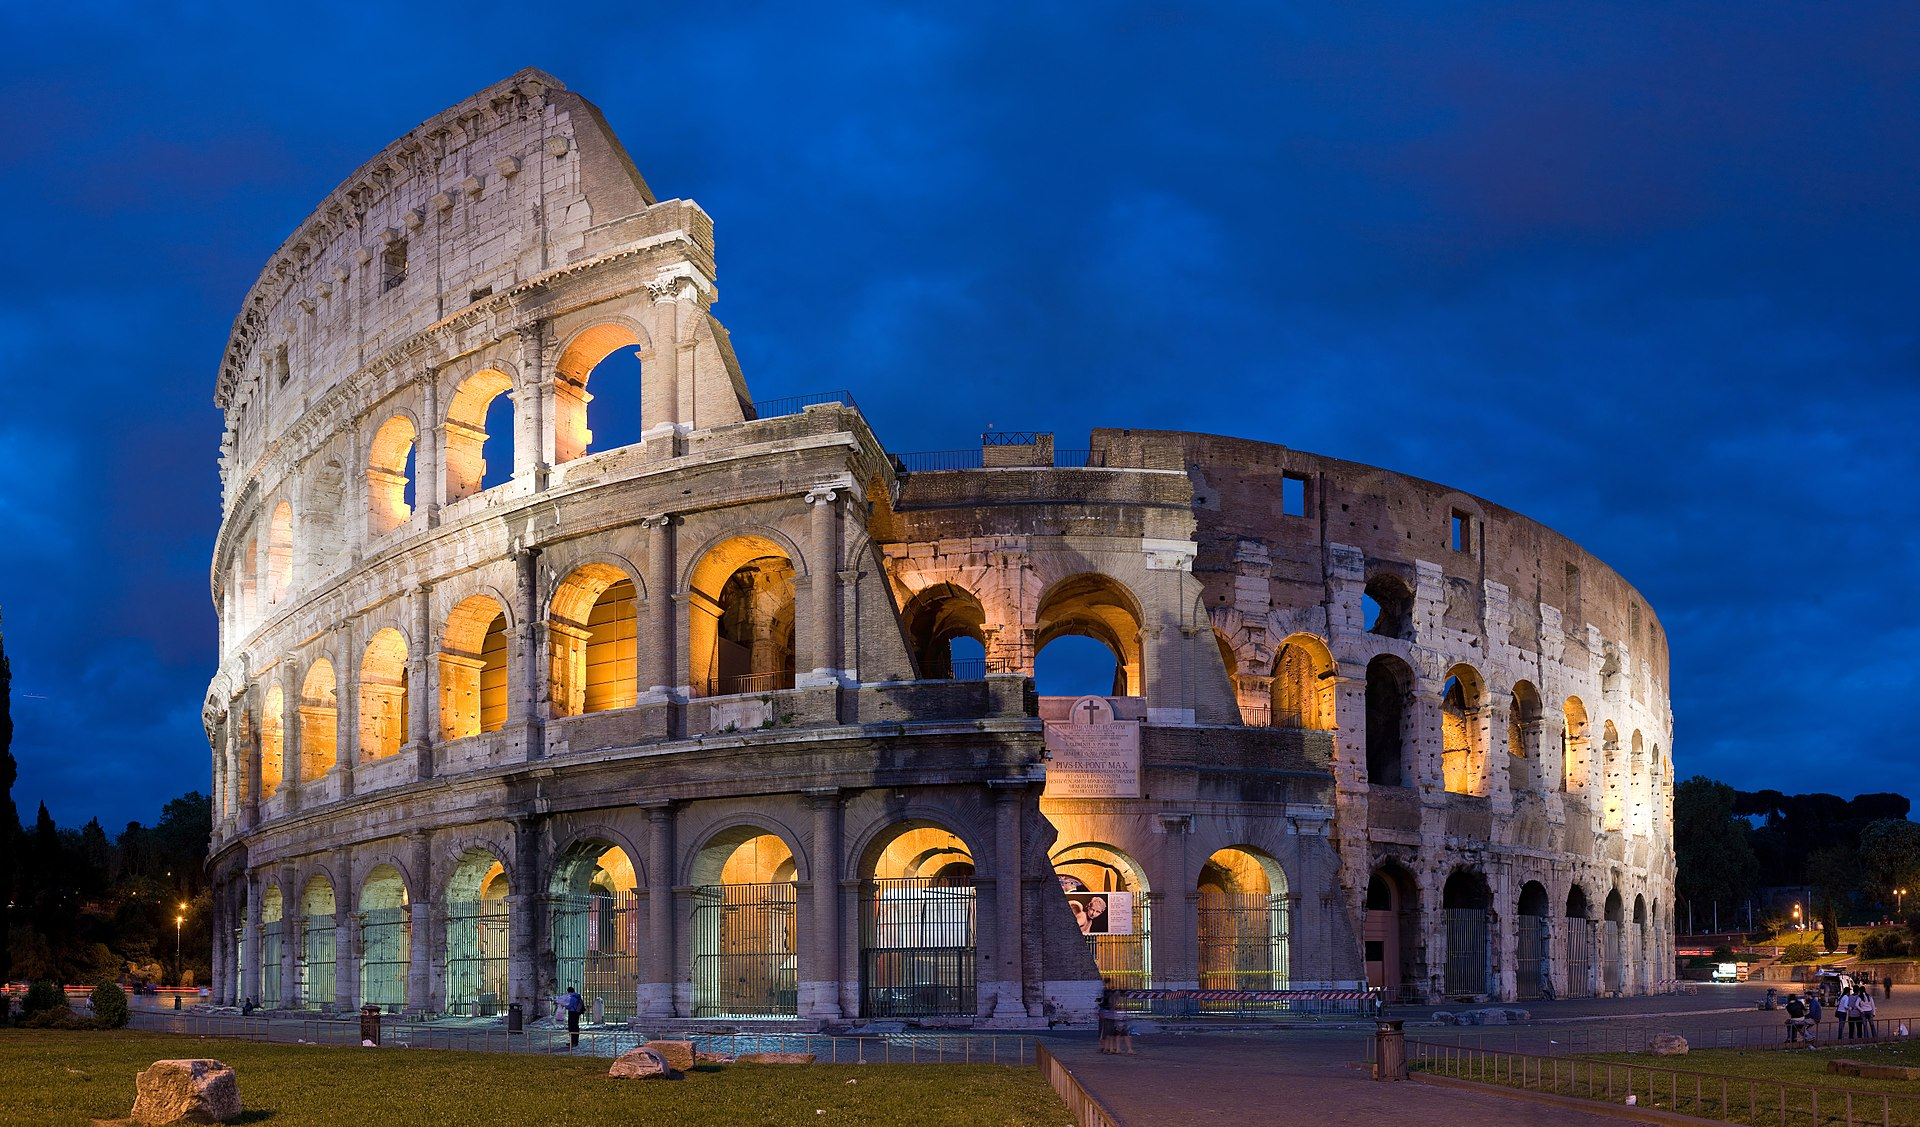
\includegraphics[width=5.5cm]{./img/coliseum.jpg}\end{center}
Construction of the Colosseum began under the rule of Vespasian in around 70–72 AD (73–75 AD according to some sources) The Colosseum had been completed up to the third story by the time of Vespasian's death in 79. The top level was finished by his son, Titus, in 80, and the inaugural games were held in AD 80 or 81. Dio Cassius recounts that over 9,000 wild animals were killed during the inaugural games of the amphitheatre. Commemorative coinage was issued celebrating the inauguration. The building was remodelled further under Vespasian's younger son, the newly designated Emperor Domitian, who constructed the hypogeum, a series of underground tunnels used to house animals and slaves. He also added a gallery to the top of the Colosseum to increase its seating capacity.\\
\indent In 217, the Colosseum was badly damaged by a major fire (caused by lightning, according to Dio Cassius) which destroyed the wooden upper levels of the amphitheatre's interior. It was not fully repaired until about 240 and underwent further repairs in 250 or 252 and again in 320. Gladiatorial fights are last mentioned around 435. An inscription records the restoration of various parts of the Colosseum under Theodosius II and Valentinian III (reigned 425–455), possibly to repair damage caused by a major earthquake in 443; more work followed in 484 and 508. The arena continued to be used for contests well into the 6th century. Animal hunts continued until at least 523, when Anicius Maximus celebrated his consulship with some venationes, criticised by King Theodoric the Great for their high cost.

%             					6th century

\part{6th century}
\chapter{541}
\section{}
\subsection{Plague of Justinian (first plague pandemic)}
\vspace{2mm}\begin{center}
\includegraphics[width=5cm]{./img/skull.jpg}\end{center}
The Plague of Justinian (541–542 AD) was a pandemic that afflicted the Eastern Roman (Byzantine) Empire, especially its capital Constantinople, the Sasanian Empire, and port cities around the entire Mediterranean Sea. One of the deadliest plagues in history, the devastating pandemic resulted in the deaths of an estimated 25–50 million people in two centuries of recurrence, equivalent to 13–26\% of the world's population at the time of the first outbreak. The plague's social and cultural impact during the period of Justinian has been compared to that of the similar Black Death that devastated Europe 600 years after the last outbreak of Justinian plague. Procopius, the principal Greek historian of the 6th century, viewed the pandemic as worldwide in scope.\\
In 2013 researchers confirmed earlier speculation that the cause of the pandemic was Yersinia pestis, the bacterium responsible for plague. Ancient and modern Yersinia pestis strains closely related to the ancestor of the Justinian plague strain have been found in Tian Shan, a system of mountain ranges on the borders of Kyrgyzstan, Kazakhstan, and China, suggesting that the Justinian plague may have originated in or near that region.

\chapter{570}
\section{}
\subsection{Birth of Muhammad}
\vspace{2mm}\begin{center}
\includegraphics[width=7cm]{./img/muhammad.jpg}\end{center}
Abu al-Qasim Muhammad ibn'Abd Allah ibn 'Abd al-Muttalib ibn Hashim, was born about the year 570 and his birthday is believed to be in the month of Rabi' al-awwal. He belonged to the Banu Hashim clan, part of the Quraysh tribe, and was one of Mecca's prominent families, although it appears less prosperous during Muhammad's early lifetime. Tradition places the year of Muhammad's birth as corresponding with the Year of the Elephant, which is named after the failed destruction of Mecca that year by the Abraha, Yemen's king, who supplemented his army with elephants. Alternatively some 20th century scholars have suggested different years, such as 568 or 569.

%             					11th century	
							
\part{11th century}
\chapter{1096}
\section{}
\subsection{Establishment of Oxford university}
\vspace{2mm}\begin{center}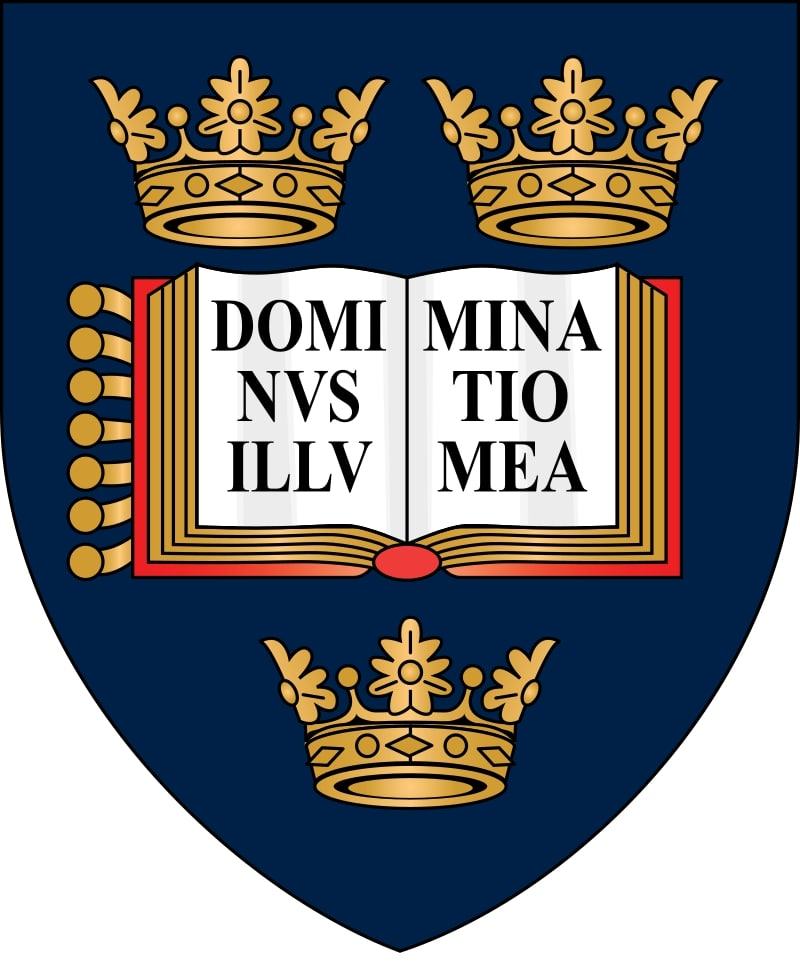
\includegraphics[width=5cm]{./img/oxfordLogo.jpg}\end{center}
The University of Oxford has no known foundation date. Teaching at Oxford existed in some form as early as 1096, but it is unclear when a university came into being. It grew quickly in 1167 when English students returned from the University of Paris. The historian Gerald of Wales lectured to such scholars in 1188 and the first known foreign scholar, Emo of Friesland, arrived in 1190. The head of the university had the title of chancellor from at least 1201, and the masters were recognised as a universitas or corporation in 1231. The university was granted a royal charter in 1248 during the reign of King Henry III.\\
After disputes between students and Oxford townsfolk in 1209, some academics fled from the violence to Cambridge, later forming the University of Cambridge.

%             					12th century	
					
\part{12th century}
\chapter{1162}
\section{}
\subsection{Birth of Genghis Khan}
\vspace{2mm}\begin{center}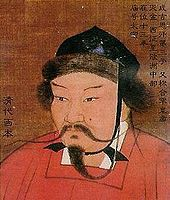
\includegraphics[width=5cm]{./img/gengishKhan.jpg}\end{center}
Little is known about Genghis Khan's early life, due to the lack of contemporary written records. The few sources that give insight into this period often contradict.\\
Genghis Khan's birth name, Temüjin, was derived from the Mongol word temür meaning "of iron", while jin denotes agency. Temüjin thus means "blacksmith".\\
Genghis Khan was probably born in 1162 in Delüün Boldog, near the mountain Burkhan Khaldun and the rivers Onon and Kherlen in modern-day northern Mongolia, close to the current capital Ulaanbaatar. The Secret History of the Mongols reports that Temüjin was born grasping a blood clot in his fist, a traditional sign that he was destined to become a great leader. He was the second son of his father Yesügei who was a Kiyad chief prominent in the Khamag Mongol confederation and an ally of Toghrul of the Keraite tribe. Temüjin was the first son of his mother Hoelun. According to the Secret History, Temüjin was named after the Tatar chief Temüjin-üge whom his father had just captured.

%             					13th century	
					
\part{13th century}
\chapter{1265}
\section{}
\subsection{Renaissance}
\vspace{2mm}\begin{center}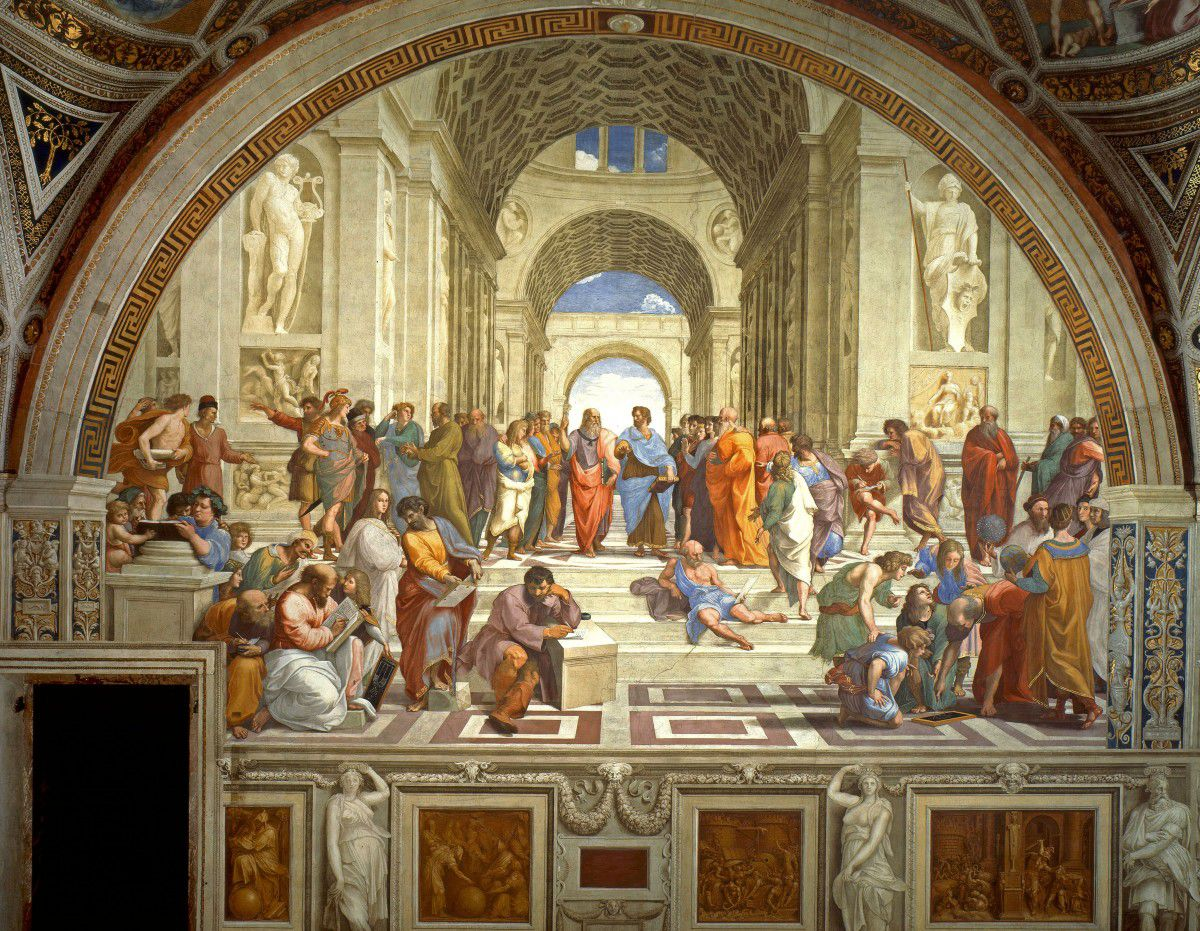
\includegraphics[width=5cm]{./img/renaissance.jpg}\end{center}
Many argue that the ideas characterizing the Renaissance had their origin in late 13th-century Florence, in particular with the writings of Dante Alighieri (1265–1321) and Petrarch (1304–1374), as well as the paintings of Giotto di Bondone (1267–1337). Some writers date the Renaissance quite precisely; one proposed starting point is 1401, when the rival geniuses Lorenzo Ghiberti and Filippo Brunelleschi competed for the contract to build the bronze doors for the Baptistery of the Florence Cathedral (Ghiberti won). Others see more general competition between artists and polymaths such as Brunelleschi, Ghiberti, Donatello, and Masaccio for artistic commissions as sparking the creativity of the Renaissance. Yet it remains much debated why the Renaissance began in Italy, and why it began when it did. Accordingly, several theories have been put forward to explain its origins.\\
During the Renaissance, money and art went hand in hand. Artists depended entirely on patrons while the patrons needed money to foster artistic talent. Wealth was brought to Italy in the 14th, 15th, and 16th centuries by expanding trade into Asia and Europe. Silver mining in Tyrol increased the flow of money. Luxuries from the Eastern world, brought home during the Crusades, increased the prosperity of Genoa and Venice.\\
Jules Michelet defined the 16th-century Renaissance in France as a period in Europe's cultural history that represented a break from the Middle Ages, creating a modern understanding of humanity and its place in the world

%             					14th century	
					
\part{14th century}
\chapter{1347}
\section{}
\subsection{Black Death (second plague pandemic)}
\vspace{2mm}\begin{center}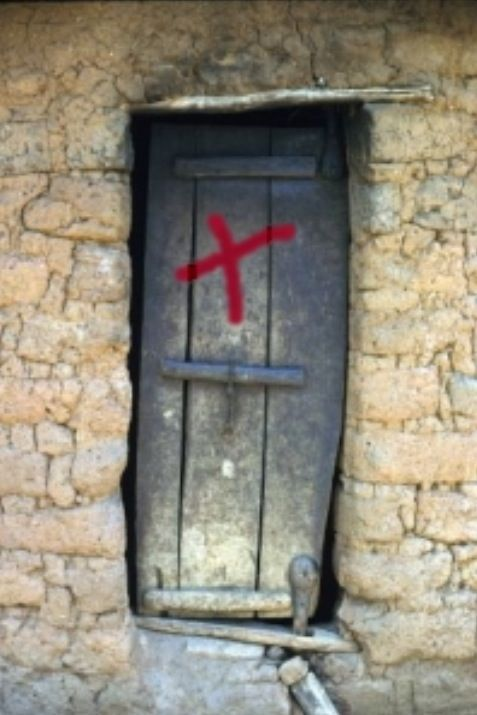
\includegraphics[width=2cm]{./img/bubonicDoor.jpg}\end{center}
In the Late Middle Ages (1340–1400) Europe experienced the most deadly disease outbreak in history when the Black Death, the infamous pandemic of bubonic plague, hit in 1347, killing a third of the European human population. Some historians believe that society subsequently became more violent as the mass mortality rate cheapened life and thus increased warfare, crime, popular revolt, waves of flagellants, and persecution. The Black Death originated in Central Asia and spread from Italy and then throughout other European countries. Arab historians Ibn Al-Wardni and Almaqrizi believed the Black Death originated in Mongolia. Chinese records also showed a huge outbreak in Mongolia in the early 1330s. Research published in 2002 suggests that it began in early 1346 in the steppe region, where a plague reservoir stretches from the northwestern shore of the Caspian Sea into southern Russia. The Mongols had cut off the trade route, the Silk Road, between China and Europe which halted the spread of the Black Death from eastern Russia to Western Europe. The epidemic began with an attack that Mongols launched on the Italian merchants' last trading station in the region, Caffa in the Crimea. In late 1346, plague broke out among the besiegers and from them penetrated into the town. When spring arrived, the Italian merchants fled on their ships, unknowingly carrying the Black Death. Carried by the fleas on rats, the plague initially spread to humans near the Black Sea and then outwards to the rest of Europe as a result of people fleeing from one area to another.

\chapter{1372}
\section{-}
\subsection{Completion of the Leaning Tower of Pisa}
\vspace{2mm}\begin{center}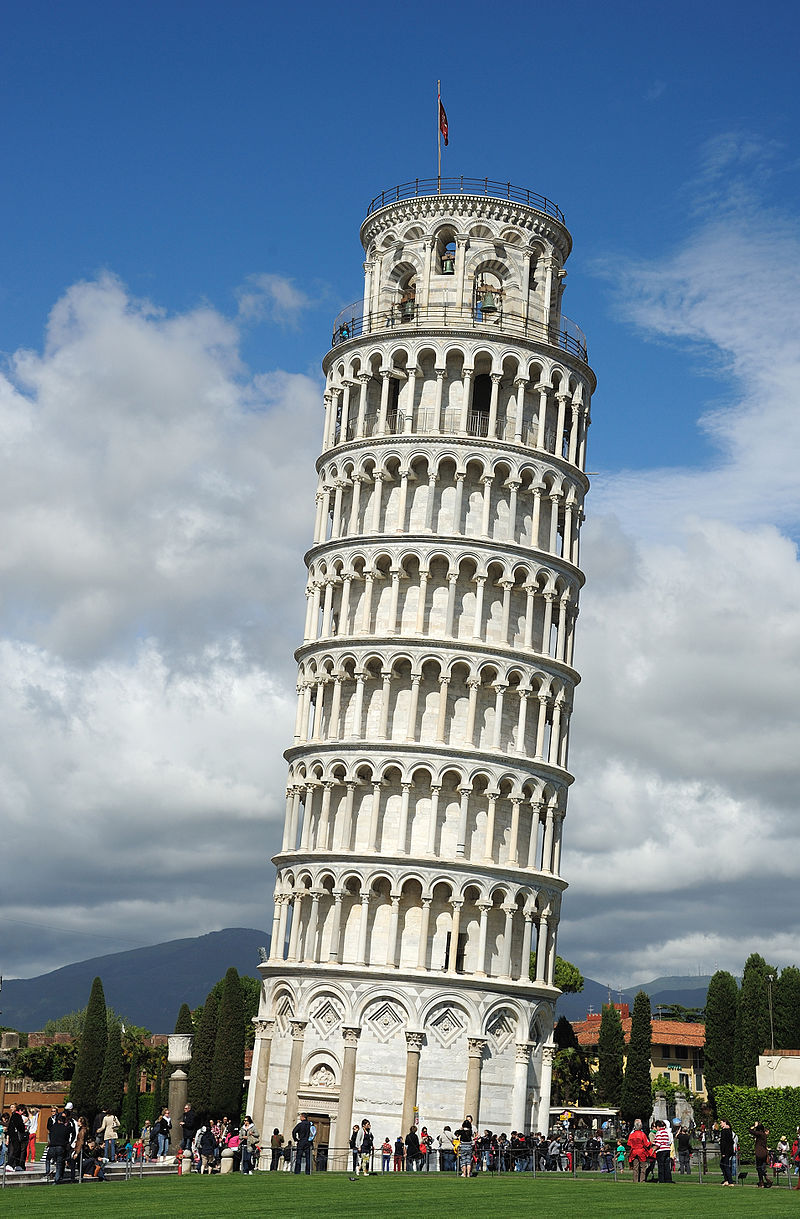
\includegraphics[width=2.7cm]{./img/towerOfPisa.jpeg}\end{center}
Construction of the tower occurred in three stages over 199 years. Work on the ground floor of the white marble campanile began on August 14, 1173 during a period of military success and prosperity. This ground floor is a blind arcade articulated by engaged columns with classical Corinthian capitals. The tower began to sink after construction had progressed to the second floor in 1178. This was due to a mere three-metre foundation, set in weak, unstable subsoil, a design that was flawed from the beginning. Construction was subsequently halted for almost a century, because the Republic of Pisa was almost continually engaged in battles with Genoa, Lucca, and Florence. This allowed time for the underlying soil to settle. Otherwise, the tower would almost certainly have toppled.\\
\indent In 1272, construction resumed under Giovanni di Simone, architect of the Camposanto. In an effort to compensate for the tilt, the engineers built upper floors with one side taller than the other. Because of this, the tower is curved. Construction was halted again in 1284 when the Pisans were defeated by the Genoans in the Battle of Meloria. The seventh floor was completed in 1319. The bell-chamber was finally added in 1372. It was built by Tommaso di Andrea Pisano, who succeeded in harmonizing the Gothic elements of the bell-chamber with the Romanesque style of the tower. There are seven bells, one for each note of the musical major scale. The largest one was installed in 1655.

%             					15th century	
					
\part{15th century}
\chapter{1400}
\section{-}
\subsection{Birth of Johannes Gutenberg}
\vspace{2mm}\begin{center}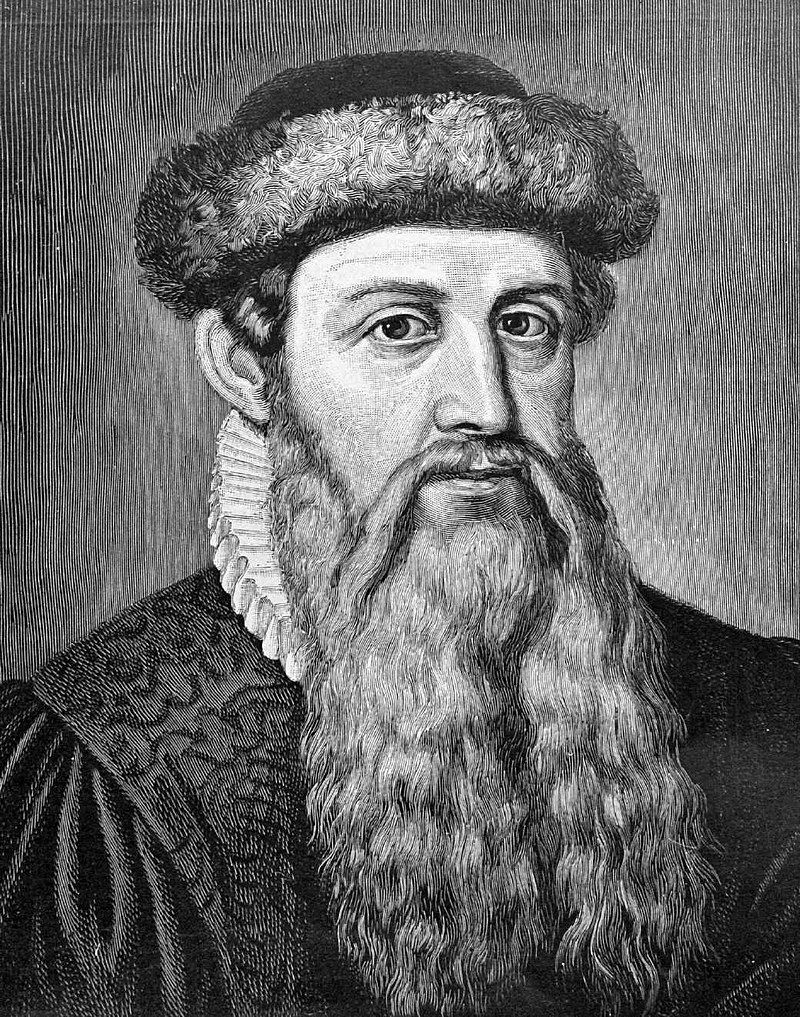
\includegraphics[width=4cm]{./img/gutenberg.jpg}\end{center}
Johannes Gensfleisch zur Laden zum Gutenberg (February 3, 1468) was a German blacksmith, goldsmith, inventor, printer, and publisher who introduced printing to Europe with the printing press. His introduction of mechanical movable type printing to Europe started the Printing Revolution and is regarded as a milestone of the second millennium, ushering in the modern period of human history. It played a key role in the development of the Renaissance, Reformation, the Age of Enlightenment, and the scientific revolution and laid the material basis for the modern knowledge-based economy and the spread of learning to the masses.\\
\indent Gutenberg was born in the German city of Mainz, the youngest son of the patrician merchant Friele Gensfleisch zur Laden, and his second wife, Else Wyrich, who was the daughter of a shopkeeper. It is assumed that he was baptized in the area close to his birthplace of St. Christoph. According to some accounts, Friele was a goldsmith for the bishop at Mainz, but most likely, he was involved in the cloth trade. Gutenberg's year of birth is not precisely known, but it was sometime between the years of 1394 and 1404. In the 1890s the city of Mainz declared his official and symbolic date of birth to be June 24, 1400.

\chapter{1453}
\section{May 29}
\subsection{The Fall of Constantinople}
\vspace{2mm}\begin{center}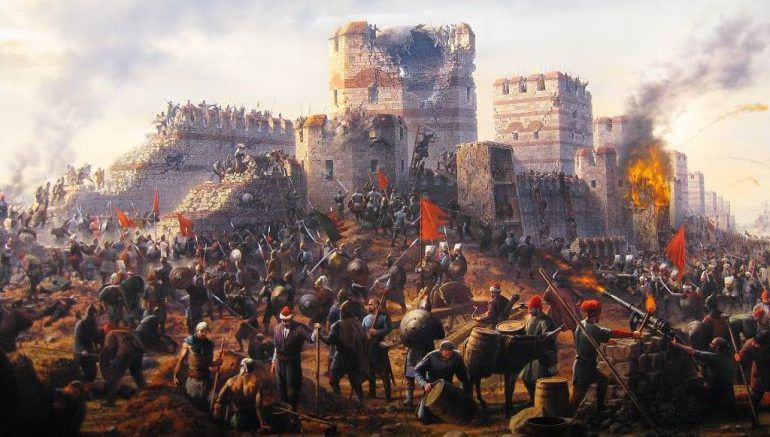
\includegraphics[width=6.5cm]{./img/fallofConstantpl.jpg}\end{center}
The Fall of Constantinople was the capture of the capital of the Byzantine Empire by an invading Ottoman army on 29 May 1453. The attackers were commanded by the 21-year-old Sultan Mehmed II, who defeated an army commanded by Emperor Constantine XI Palaiologos and took control of the imperial capital, ending a 53-day siege that began on 6 April 1453. After conquering the city, Sultan Mehmed transferred the capital of his Empire from Edirne to Constantinople and established his court there.\\
The capture of the city (and two other Byzantine splinter territories soon thereafter) marked the end of the Byzantine Empire, a continuation of the Roman Empire, an imperial state dating to 27 BC, which had lasted for nearly 1,500 years. The conquest of Constantinople also dealt a massive blow to Christendom, as the Muslim Ottoman armies thereafter were left unchecked to advance into Europe without an adversary to their rear.\\
It was also a watershed moment in military history. Since ancient times, cities had used ramparts and city walls to protect themselves from invaders, and Constantinople's substantial fortifications had been a model followed by cities throughout the Mediterranean region and Europe. The Ottomans ultimately prevailed due to the use of gunpowder (which powered formidable cannons).\\
The conquest of the city of Constantinople and the end of the Byzantine Empire was a key event in the Late Middle Ages which also marks, for some historians, the end of the Medieval period.

\chapter{1492}
\section{August 3}
\subsection{Sailing of Christopher Colombus to America}
\vspace{2mm}\begin{center}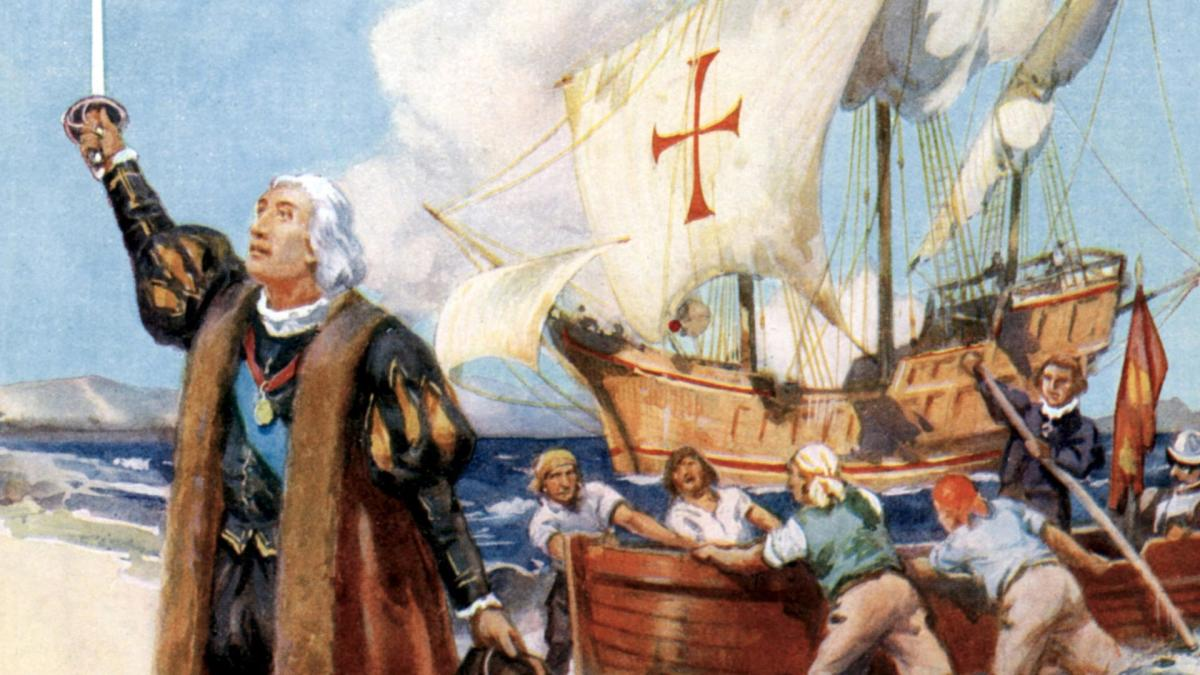
\includegraphics[width=7cm]{./img/colombus.jpg}\end{center}
On the evening of 3 August 1492, Columbus departed from Palos de la Frontera with three ships.\\ \indent Columbus first sailed to the Canary Islands, which belonged to Castile. He restocked provisions and made repairs in Gran Canaria, then departed from San Sebastián de La Gomera on 6 September, for what turned out to be a five-week voyage across the ocean. At about 2:00 in the morning of 12 October (21 October, Gregorian Calendar New Style), a lookout on the Pinta, Rodrigo de Triana (also known as Juan Rodríguez Bermeo), spotted land, and immediately alerted the rest of the crew with a shout. Thereupon, the captain of the Pinta, Martín Alonso Pinzón, verified the discovery and alerted Columbus by firing a lombard. Columbus later maintained that he himself had already seen a light on the land a few hours earlier, thereby claiming for himself the lifetime pension promised by Ferdinand and Isabella to the first person to sight land.\\
\indent Columbus called the island (in what is now the Bahamas) San Salvador (meaning "Holy Savior"); the natives called it Guanahani. Exactly which island in the Bahamas this corresponds to is unresolved. Based on primary accounts and on what one would expect from the geographic positions of the islands given Columbus's course, the prime candidates are San Salvador Island (so named in 1925 on the theory that it was Columbus's San Salvador), Samana Cay, and Plana Cays.

%             					16th century	
								
\part{16th century}
\chapter{1543}
\section{}
\subsection{Modern scientific revolution}
\vspace{2mm}\begin{center}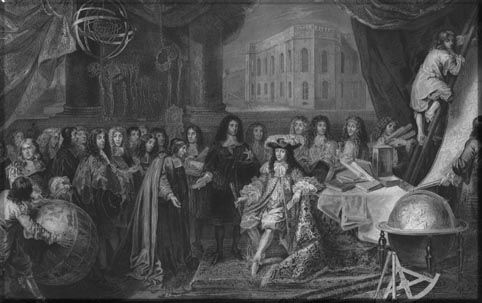
\includegraphics[width=10cm]{./img/screvolution.jpg}\end{center}
The Scientific Revolution was a series of events that marked the emergence of modern science during the early modern period, when developments in mathematics, physics, astronomy, biology (including human anatomy) and chemistry transformed the views of society about nature. The Scientific Revolution took place in Europe towards the end of the Renaissance period and continued through the late 18th century, influencing the intellectual social movement known as the Enlightenment. While its dates are debated, the publication in 1543 of Nicolaus Copernicus's De revolutionibus orbium coelestium (On the Revolutions of the Heavenly Spheres) is often cited as marking the beginning of the Scientific Revolution.

\chapter{1564}
\section{February 15}
\subsection{Birth of Galileo Galilei}
\vspace{2mm}\begin{center}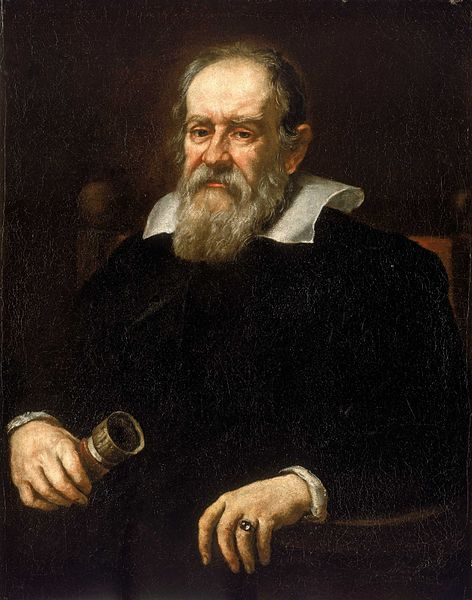
\includegraphics[width=4.5cm]{./img/galileo.jpg}\end{center}
Galileo was born in Pisa (then part of the Duchy of Florence), Italy, on 15 February 1564, the first of six children of Vincenzo Galilei, a famous lutenist, composer, and music theorist, and Giulia (née Ammannati), who had married in 1562. Galileo became an accomplished lutenist himself and would have learned early from his father a scepticism for established authority, the value of well-measured or quantified experimentation, an appreciation for a periodic or musical measure of time or rhythm, as well as the results expected from a combination of mathematics and experiment.\\
Three of Galileo's five siblings survived infancy. The youngest, Michelangelo (or Michelagnolo), also became a noted lutenist and composer although he contributed to financial burdens during Galileo's young adulthood. Michelangelo was unable to contribute his fair share of their father's promised dowries to their brothers-in-law, who would later attempt to seek legal remedies for payments due. Michelangelo would also occasionally have to borrow funds from Galileo to support his musical endeavours and excursions. These financial burdens may have contributed to Galileo's early desire to develop inventions that would bring him additional income.

%             					17th century
		
\part{17th century}
\chapter{1636}
\subsection{Establishment of Harvard university}
\vspace{2mm}\begin{center}
\includegraphics[width=5cm]{./img/harvardLogo.jpg}\end{center}
Harvard was established in 1636 by vote of the Great and General Court of the Massachusetts Bay Colony. In 1638, it acquired British North America's first known printing press. In 1639, it was named Harvard College after deceased clergyman John Harvard, an alumnus of the University of Cambridge, who had left the school £779 and his scholar's library of some 400 volumes. The charter creating the Harvard Corporation was granted in 1650.\\
A 1643 publication gave the school's purpose as "to advance learning and perpetuate it to posterity, dreading to leave an illiterate ministry to the churches when our present ministers shall lie in the dust"; in its early years trained many Puritan ministers. It offered a classic curriculum on the English university model-many leaders in the colony had attended the University of Cambridge-but conformed to the tenets of Puritanism. It was never affiliated with any particular denomination, but many of its earliest graduates went on to become clergymen in Congregational and Unitarian churches.\\
The leading Boston divine Increase Mather served as president from 1685 to 1701. In 1708, John Leverett became the first president who was not also a clergyman, marking a turning of the college from Puritanism and toward intellectual independence.

\chapter{1642}
\section{January 08}
\subsection{Death of Galileo Galilei}
\vspace{2mm}\begin{center}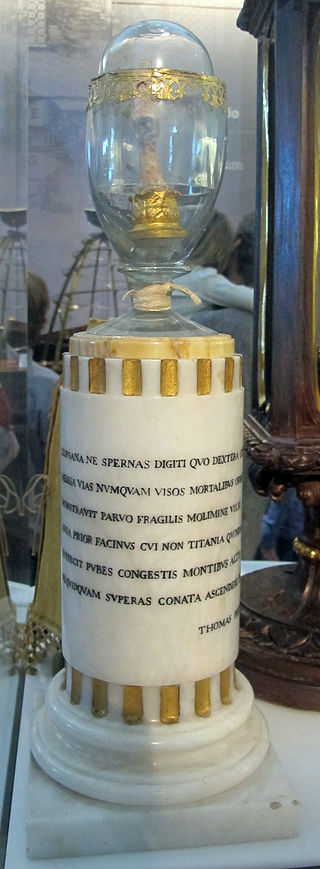
\includegraphics[width=2.5cm]{./img/galileoMiddleFinger.jpg}\end{center}
Galileo continued to receive visitors until 1642, when, after suffering fever and heart palpitations, he died on 8 January 1642, aged 77. The Grand Duke of Tuscany, Ferdinando II, wished to bury him in the main body of the Basilica of Santa Croce, next to the tombs of his father and other ancestors, and to erect a marble mausoleum in his honour.\\
These plans were dropped, however, after Pope Urban VIII and his nephew, Cardinal Francesco Barberini, protested, because Galileo had been condemned by the Catholic Church for "vehement suspicion of heresy". He was instead buried in a small room next to the novices' chapel at the end of a corridor from the southern transept of the basilica to the sacristy. He was reburied in the main body of the basilica in 1737 after a monument had been erected there in his honour; during this move, three fingers and a tooth were removed from his remains. One of these fingers, the middle finger from Galileo's right hand, is currently on exhibition at the Museo Galileo in Florence, Italy.

\chapter{1643}
\section{January 04}
\subsection{Birth of Sir Isaac Newton}
\vspace{2mm}\begin{center}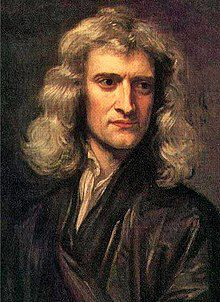
\includegraphics[width=5cm]{./img/isaacNewton.jpg}\end{center}
Sir Isaac Newton was an English mathematician, physicist, astronomer, theologian, and author (described in his own day as a "natural philosopher") who is widely recognized as one of the most influential scientists of all time, and a key figure in the scientific revolution. His book Philosophiæ Naturalis Principia Mathematica ("Mathematical Principles of Natural Philosophy"), first published in 1687, laid the foundations of classical mechanics. Newton also made seminal contributions to optics, and shares credit with Gottfried Wilhelm Leibniz for developing the infinitesimal calculus.
\section{-}
\subsection{Completion of the Taj Mahal}
\vspace{2mm}\begin{center}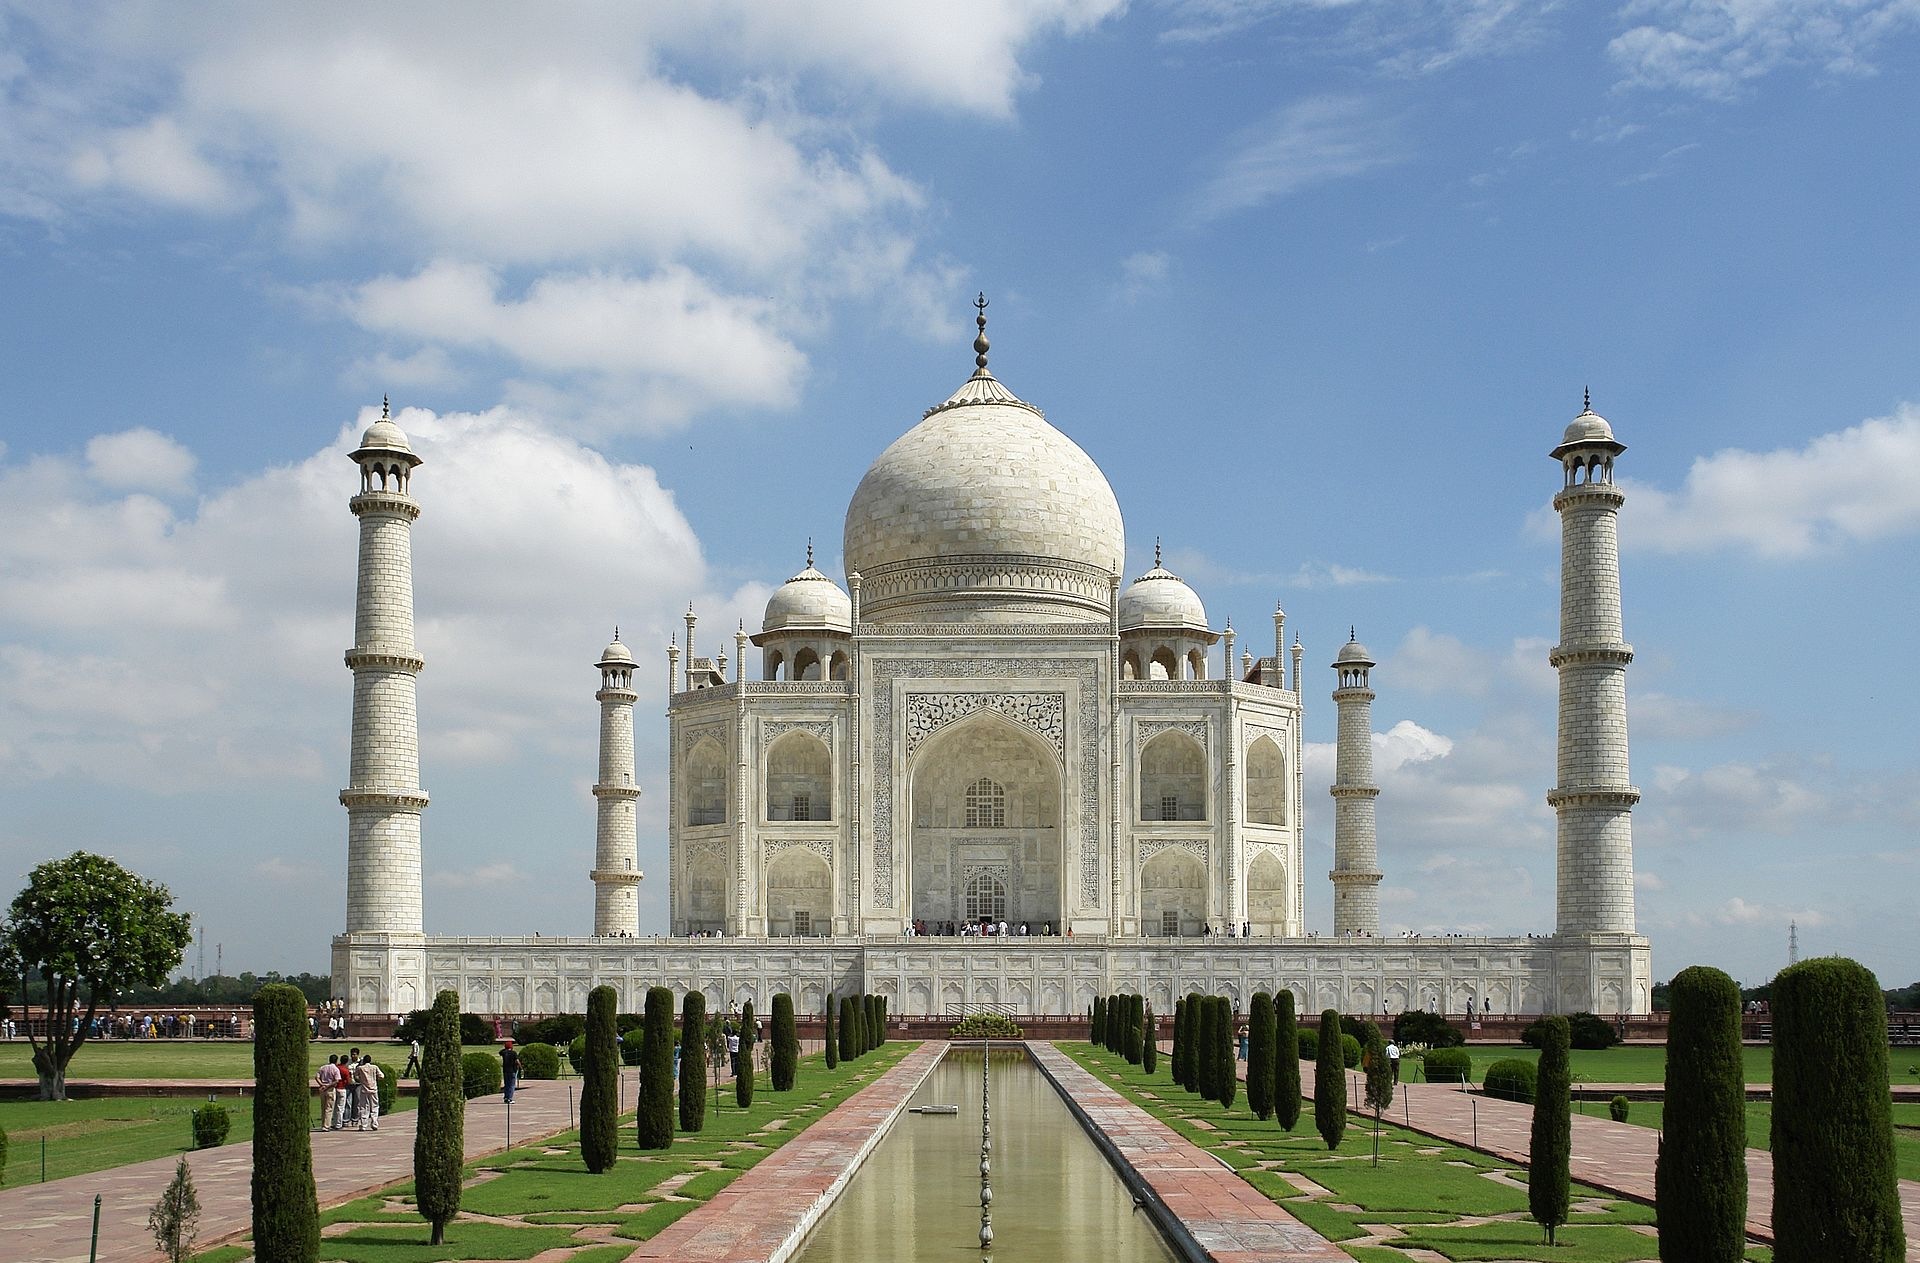
\includegraphics[width=5cm]{./img/tajMahal.jpeg}\end{center}
The Taj Mahal is built on a parcel of land to the south of the walled city of Agra. Shah Jahan presented Maharajah Jai Singh with a large palace in the centre of Agra in exchange for the land. An area of roughly 1.2 hectares (3 acres) was excavated, filled with dirt to reduce seepage, and levelled at 50 metres (160 ft) above riverbank. In the tomb area, wells were dug and filled with stone and rubble to form the footings of the tomb. Instead of lashed bamboo, workmen constructed a colossal brick scaffold that mirrored the tomb. The scaffold was so enormous that foremen estimated it would take years to dismantle.\\
\indent The Taj Mahal was constructed using materials from all over India and Asia. It is believed over 1,000 elephants were used to transport building materials. It took efforts from 22,000 labourer, painters, embroidery artists and stonecutters to shape the Taj Mahal. The translucent white marble was brought from Makrana, Rajasthan, the jasper from Punjab, jade and crystal from China. The turquoise was from Tibet and the Lapis lazuli from Afghanistan, while the sapphire came from Sri Lanka and the carnelian from Arabia. In all, twenty-eight types of precious and semi-precious stones were inlaid into the white marble.\\
\indent The plinth and tomb took roughly 12 years to complete. The remaining parts of the complex took an additional 10 years and were completed in order of minarets, mosque and jawab, and gateway. Since the complex was built in stages, discrepancies exist in completion dates due to differing opinions on "completion". Construction of the mausoleum itself was essentially completed by 1643 while work continued on the outlying buildings continued for years. Estimates of the cost of construction vary due to difficulties in estimating costs across time. The total cost at the time has been estimated to be about 32 million Indian rupees, which is around 52.8 billion Indian rupees (\$827 million US) based on 2015 values.

%             					18th century
							
\part{18th century}
\chapter{1760}
\section{}
\subsection{Industrial revolution}
The Industrial Revolution was the transition to new manufacturing processes in Europe and the US, in the period from about 1760 to sometime between 1820 and 1840. This transition included going from hand production methods to machines, new chemical manufacturing and iron production processes, the increasing use of steam power, the development of machine tools and the rise of the factory system. The Industrial Revolution also led to an unprecedented rise in the rate of population growth.\\
\indent The Industrial Revolution began in Great Britain, and many of the technological innovations were of British origin. By the mid-18th century Britain was the world's leading commercial nation, controlling a global trading empire with colonies in North America and the Caribbean, and with some political influence on the Indian subcontinent, through the activities of the East India Company. The development of trade and the rise of business were major causes of the Industrial Revolution.\\
\indent The Industrial Revolution marks a major turning point in history; almost every aspect of daily life was influenced in some way. In particular, average income and population began to exhibit unprecedented sustained growth. Some economists say that the major impact of the Industrial Revolution was that the standard of living for the general population began to increase consistently for the first time in history, although others have said that it did not begin to meaningfully improve until the late 19th and 20th centuries.\\
\indent GDP per capita was broadly stable before the Industrial Revolution and the emergence of the modern capitalist economy, while the Industrial Revolution began an era of per-capita economic growth in capitalist economies. Economic historians are in agreement that the onset of the Industrial Revolution is the most important event in the history of humanity since the domestication of animals and plants.

\chapter{1769}
\section{August 15}
\subsection{Birth of Napoleon Bonaparte}
\vspace{2mm}\begin{center}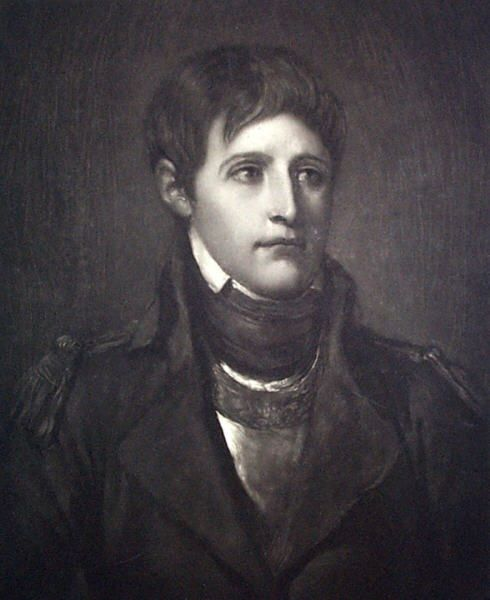
\includegraphics[width=5cm]{./img/youngBonaparte.jpg}\end{center}
Napoleon was born the same year the Republic of Genoa, a former commune of Italy, transferred Corsica to France. The state sold sovereign rights a year before his birth in 1768, and the island was conquered by France during the year of his birth and formally incorporated as a province in 1770, after 500 years under nominal Genoese rule and 14 years of independence. Napoleon's parents fought to maintain independence even when Maria was pregnant with him. His father was an attorney who went on to be named Corsica's representative to the court of Louis XVI in 1777. The dominant influence of Napoleon's childhood was his mother, whose firm discipline restrained a rambunctious child.
Later in life Napoleon noted, "The future destiny of the child is always the work of the mother." Napoleon's maternal grandmother had married into the Swiss Fesch family in her second marriage, and Napoleon's uncle, the cardinal Joseph Fesch, would fulfill a role as protector of the Bonaparte family for some years. Napoleon's noble, moderately affluent background afforded him greater opportunities to study than were available to a typical Corsican of the time.

\chapter{1776}
\section{July 04}
\subsection{Independence of the United States}
\vspace{2mm}\begin{center}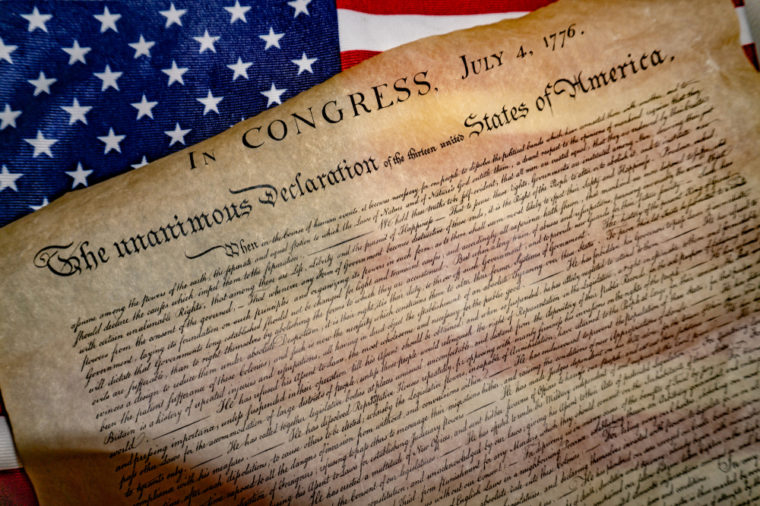
\includegraphics[width=4.5cm]{./img/usaIndep.jpg}\end{center}
The United States Declaration of Independence is the statement adopted by the Second Continental Congress meeting at the Pennsylvania State House (now known as Independence Hall) in Philadelphia, Pennsylvania on July 4, 1776. The Declaration announced that the Thirteen Colonies at war with the Kingdom of Great Britain would regard themselves as thirteen independent sovereign states, no longer under British rule. With the Declaration, these new states took a collective first step toward forming the United States of America. The declaration was signed by representatives from New Hampshire, Massachusetts Bay, Rhode Island, Connecticut, New York, New Jersey, Pennsylvania, Maryland, Delaware, Virginia, North Carolina, South Carolina, and Georgia.\\
The Lee Resolution for independence was passed on July 2 with no opposing votes. The Committee of Five had drafted the Declaration to be ready when Congress voted on independence. John Adams, a leader in pushing for independence, had persuaded the committee to select Thomas Jefferson to compose the original draft of the document, which Congress edited to produce the final version. The Declaration was a formal explanation of why Congress had voted to declare independence from Great Britain, more than a year after the outbreak of the American Revolutionary War. Adams wrote to his wife Abigail, "The Second Day of July 1776, will be the most memorable Epocha, in the History of America" – although Independence Day is actually celebrated on July 4, the date that the wording of the Declaration of Independence was approved.
\chapter{1796}
\section{May 14}
\subsection{Invention of the Smallpox vaccine (first vaccine)}
\vspace{2mm}\begin{center}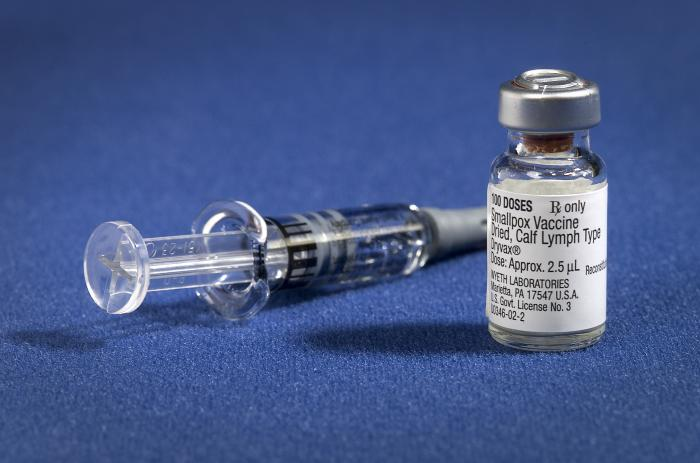
\includegraphics[width=8cm]{./img/smallpoxVaccine.jpg}\end{center}
Edward Jenner, (17 May 1749 – 26 January 1823) was an English physician and scientist who was the pioneer of smallpox vaccine, the world's first vaccine. The terms "vaccine" and "vaccination" are derived from Variolae vaccinae (smallpox of the cow), the term devised by Jenner to denote cowpox. He used it in 1796 in the long title of his Inquiry into the Variolae vaccinae known as the Cow Pox, in which he described the protective effect of cowpox against smallpox.\\
\indent Jenner is often called "the father of immunology", and his work is said to have "saved more lives than the work of any other human". In Jenner’s time, smallpox killed around 10 percent of the population, with the number as high as 20 percent in towns and cities where infection spread more easily. In 1821 he was appointed physician extraordinary to King George IV, and was also made mayor of Berkeley and justice of the peace. A member of the Royal Society, in the field of zoology he was the first person to describe the brood parasitism of the cuckoo. In 2002, Jenner was named in the BBC's list of the 100 Greatest Britons.

%             					19th century	
						
\part{19th century}
\chapter{1800}
\section{November 01}
\subsection{Completion of the White House}
\vspace{2mm}\begin{center}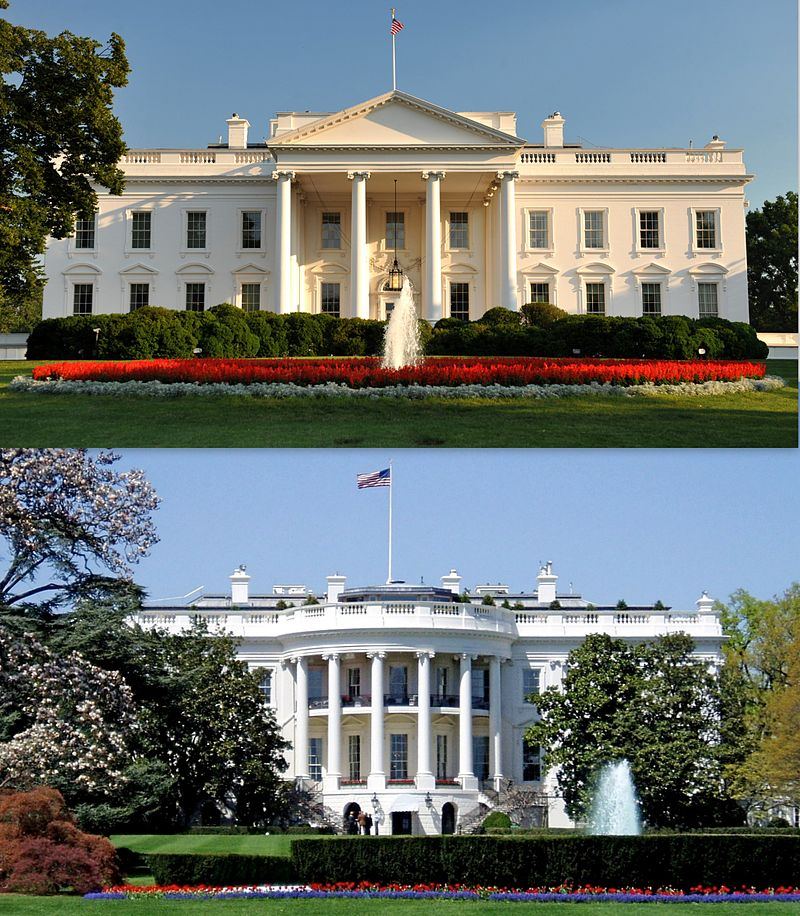
\includegraphics[width=3cm]{./img/whiteHouse.jpg}\end{center}
Following his April 1789 inauguration, President George Washington occupied two executive mansions in New York City: the Samuel Osgood House at 3 Cherry Street (April 1789 – February 1790), and the Alexander Macomb House at 39–41 Broadway (February–August 1790). In May 1790, New York began construction of Government House for his official residence, but he never occupied it. The national capital moved to Philadelphia in December 1790.\\
\indent The July 1790 Residence Act named Philadelphia, Pennsylvania the temporary national capital for a 10-year period while the Federal City was under construction. The City of Philadelphia rented Robert Morris's city house at 190 High Street (now 524–30 Market Street) for Washington's presidential residence.\\
\indent The first U.S. President occupied the Market Street mansion from November 1790 to March 1797 and altered it in ways that may have influenced the design of the White House. As part of a futile effort to have Philadelphia named the permanent national capital, Pennsylvania built a much grander presidential mansion several blocks away, but Washington declined to occupy it.\\
\indent President John Adams also occupied the Market Street mansion from March 1797 to May 1800. On Saturday, November 1, 1800, he became the first president to occupy the White House. The President's House in Philadelphia became a hotel and was demolished in 1832, while the unused presidential mansion became home to the University of Pennsylvania.

\chapter{1802}
\section{February 26}
\subsection{Birth of Victor Hugo}
\vspace{2mm}\begin{center}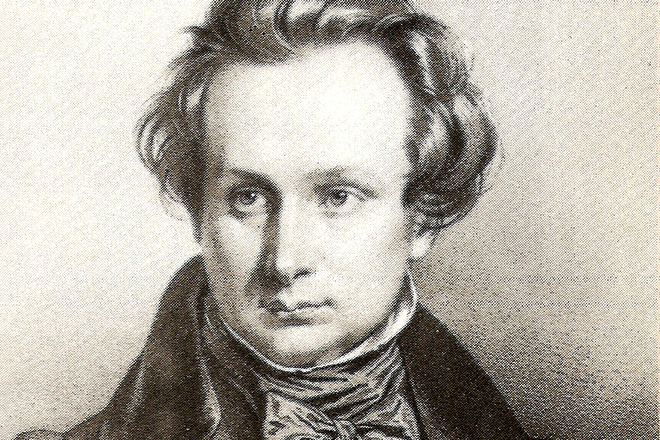
\includegraphics[width=7cm]{./img/youngHugo.jpg}\end{center}
Victor Hugo was the third son of Joseph Léopold Sigisbert Hugo (1774–1828) and Sophie Trébuchet (1772–1821); his brothers were Abel Joseph Hugo (1798–1855) and Eugène Hugo (1800–1837). He was born in 1802 in Besançon in the eastern region of Franche-Comté. On 19 November 1821, Léopold Hugo wrote to his son that he had been conceived on one of the highest peaks in the Vosges Mountains, on a journey from Lunéville to Besançon. " This elevated origin, he went on, seems to have had effects on you so that your muse is now continually sublime." Léopold Hugo was a freethinking republican who considered Napoleon a hero; by contrast, Sophie Hugo was a Catholic Royalist who was intimately involved with her possible lover General Victor Lahorie, who was executed in 1812 for plotting against Napoleon.\\
Hugo's childhood was a period of national political turmoil. Napoleon was proclaimed Emperor of the French two years after Hugo's birth, and the Bourbon Monarchy was restored before his 13th birthday. The opposing political and religious views of Hugo's parents reflected the forces that would battle for supremacy in France throughout his life: Hugo's father was a high-ranking officer in Napoleon's army until he failed in Spain (one of the reasons why his name is not present on the Arc de Triomphe).

\chapter{1821}
\section{December 25}
\subsection{Birth of Clara Harlowe Barton}
\vspace{2mm}\begin{center}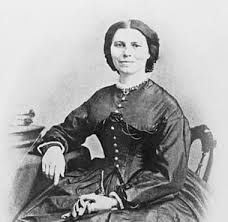
\includegraphics[width=5cm]{./img/claraBarton.jpg}\end{center}
Clarissa "Clara" Harlowe Barton (December 25, 1821 – April 12, 1912) was a pioneering nurse who founded the American Red Cross. She was a hospital nurse in the American Civil War, a teacher, and patent clerk. Nursing education was not very formalized at that time and she did not attend nursing school, so she provided self-taught nursing care. Barton is noteworthy for doing humanitarian work at a time when relatively few women worked outside the home. She was inducted into the National Women's Hall of Fame in 1973.\\ \indent Clara Barton was born on December 25, 1821, in North Oxford, Massachusetts. Her father was Captain Stephen Barton, a member of the local militia and a selectman who inspired his daughter with patriotism and a broad humanitarian interest. He was a soldier under the command of General Anthony Wayne in his crusade against the Indians in the northwest. He was also the leader of progressive thought in the Oxford village area. Barton's mother was Sarah Stone Barton.\\
\indent When she was three years old, Barton was sent to school with her brother Stephen, where she excelled in reading and spelling. At school, she became close friends with Nancy Fitts; she is the only known friend Barton had as a child due to her extreme timidity.

\chapter{1841}
\section{April 06}
\subsection{Inauguration of John Tyler}
\vspace{2mm}\begin{center}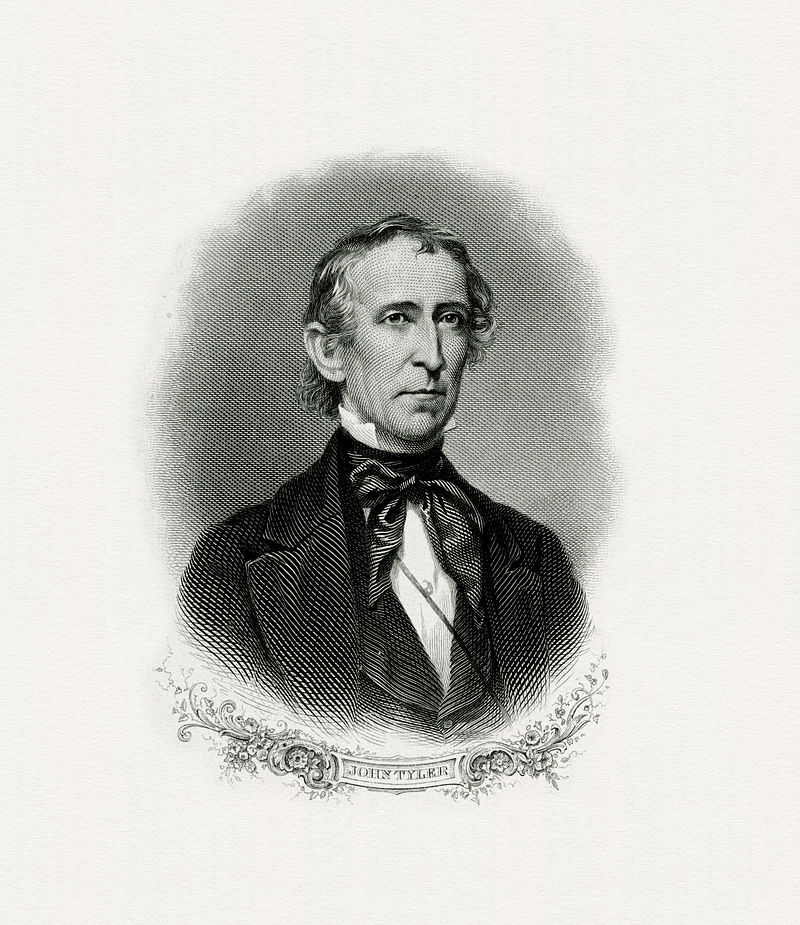
\includegraphics[width=3cm]{./img/johnTyler.jpg}\end{center}
The inauguration of John Tyler as the tenth President of the United States was held on Tuesday, April 6, 1841 at the Brown’s Indian Queen Hotel in Washington, D.C., following the death of President William Henry Harrison two days earlier. The inauguration marked the commencement of John Tyler's only term (a partial term of 3 years, 334 days) as President. William Cranch, chief judge of the United States Circuit Court of the District of Columbia, administered the presidential oath of office to Tyler. This was the first time in American history that the death of a president had occasioned the swearing-in of a new president.\\
\indent On March 26, 1841, President Harrison came down with a cold, then pneumonia and pleurisy set in. It was believed that his illness was directly caused by the bad weather at his inauguration on March 4; however, Harrison's illness did not arise until more than three weeks after the event.\\
\indent On April 1, Secretary of State Daniel Webster sent word of Harrison's illness to Tyler, who was at his home in Williamsburg, Virginia. Two days later, Richmond attorney James Lyons wrote with the news that the president had taken a turn for the worse, remarking that "I shall not be surprised to hear by tomorrow's mail that Gen'l Harrison is no more." Tyler determined not to travel to Washington, not wanting to appear unseemly in anticipating the president's death. At dawn on April 5, Webster's son Fletcher, Chief Clerk of the State Department, arrived at Tyler's plantation with a letter from Webster, informing the new president of Harrison's death the morning before.
\section{-}
\subsection{Founding of C\&A}
\vspace{2mm}\begin{center}
\includegraphics[width=5cm]{./img/c&aLogo.jpg}\end{center}
The company was founded by brothers Clemens and August Brenninkmeijer in 1841 as a Dutch textile company, taking its company name from their initials. In 1906 Clemens' son, Bernard Joseph, started discounting in Amsterdam (Rekenen in Centen, in plaats van Procenten) and by 1910 there were ten stores in the Netherlands. These were from the German Brenninkmeyer family that traded in linen and textiles since the 17th century from its hometown of Mettingen, Germany.\\
For many years, C\&A retail clothing stores were a major presence in town centres throughout the United Kingdom. C\&A also opened stores in a number of out-of-town locations, most notably its store at the Merry Hill Shopping Centre in the West Midlands, which opened in November 1989. The company's strategy of selling budget clothes from high-rent city-centre retail stores made it vulnerable to a new breed of competitors operating in cheaper, out-of-town locations, including Matalan and the rapidly expanding clothing operations of supermarket food chains such as Tesco and Asda, and to expanding high street names such as H\&M, Zara, and Topshop. C\&A in the United Kingdom was a notable example of an incorporated private unlimited company, which meant that it was not required to publish its financial statements under United Kingdom company law. In 2000, C\&A announced its intention to withdraw from the British market, where it had been operating since 1922, and the last UK retail stores closed in 2001. Primark bought 11 of the C\&A stores.

\chapter{Mid 19th century}
\section{}
\subsection{Modern pandemic (third plague pandemic)}
%\vspace{2mm}\begin{center}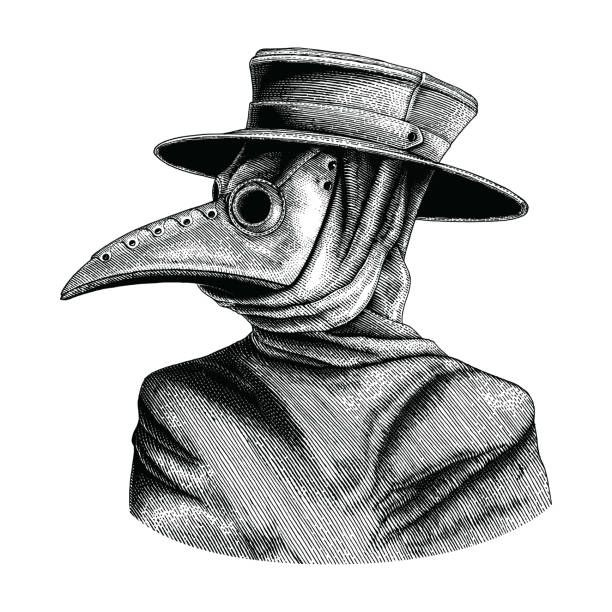
\includegraphics[width=1cm]{./img/bubonicDoc.jpg}\end{center}
The plague resurfaced for a third time in the mid-19th century. Like the two previous outbreaks, this one also originated in Eastern Asia, most likely in Yunnan Province of China, where there are several natural plague foci. The initial outbreaks occurred in the second half of the eighteenth century. The disease remained localized in Southwest China for several years before spreading. In the city of Canton, beginning in January 1894, the disease killed 80,000 people by June. Daily water-traffic with the nearby city of Hong Kong rapidly spread the plague there, killing over 2,400 within two months.\\
Also known as the modern pandemic, the third pandemic spread the disease to port cities throughout the world in the second half of the 19th century and early 20th century via shipping routes. The plague inflicted people in Chinatown in San Francisco from 1900-1904, and the people of Oakland and east bay again from 1907-1909. During the outbreak from 1900-1904 in San Francisco is when authorities made permanent the Chinese Exclusion Act. This law was originally signed into existence by President Chester A. Arthur in 1882. The Chinese Exclusion Act was supposed to last for ten years but was renewed in 1892 with the Geary Act and subsequently made permanent in 1902 during the outbreak of plague in Chinatown, San Francisco. The last major outbreak in the United States occurred in Los Angeles in 1924, though the disease is still present in wild rodents, and can be passed to humans that come in contact with them. According to the World Health Organization, the pandemic was considered active until 1959, when worldwide casualties dropped to 200 per year. In 1994, a plague outbreak in five Indian states caused an estimated 700 infections (including 52 deaths) and triggered a large migration of Indians within India as they tried to avoid the plague.

\chapter{1854}
\section{}
\subsection{Founding of Louis Vuitton}
\vspace{2mm}\begin{center}
\includegraphics[width=5cm]{./img/LouisVuittonLogo.jpg}\end{center}
The Louis Vuitton label was founded by Vuitton in 1854 on Rue Neuve des Capucines in Paris, France. Louis Vuitton had observed that the HJ Cave Osilite trunk could be easily stacked. In 1858, Vuitton introduced his flat-topped trunks with trianon canvas, making them lightweight and airtight. Before the introduction of Vuitton's trunks, rounded-top trunks were used, generally to promote water runoff, and thus could not be stacked. It was Vuitton's gray Trianon canvas flat trunk that allowed the ability to stack with ease for voyages. Many other luggage makers imitated LV's style and design.\\
The company participated in the 1867 Universal Exhibition in Paris. To protect against the duplication of his look, Vuitton changed the Trianon design to a beige and brown stripes design in 1876. By 1885, the company opened its first store in London on Oxford Street. Soon thereafter, due to the continuing imitation of his look, in 1888, Vuitton created the Damier Canvas pattern, which bore a logo that reads "marque L. Vuitton déposée", which translates into "L. Vuitton registered trademark". In 1892, Louis Vuitton died, and the company's management passed to his son.

\chapter{1861}
\section{March 04}
\subsection{Inauguration of Abraham Lincoln}
\vspace{2mm}\begin{center}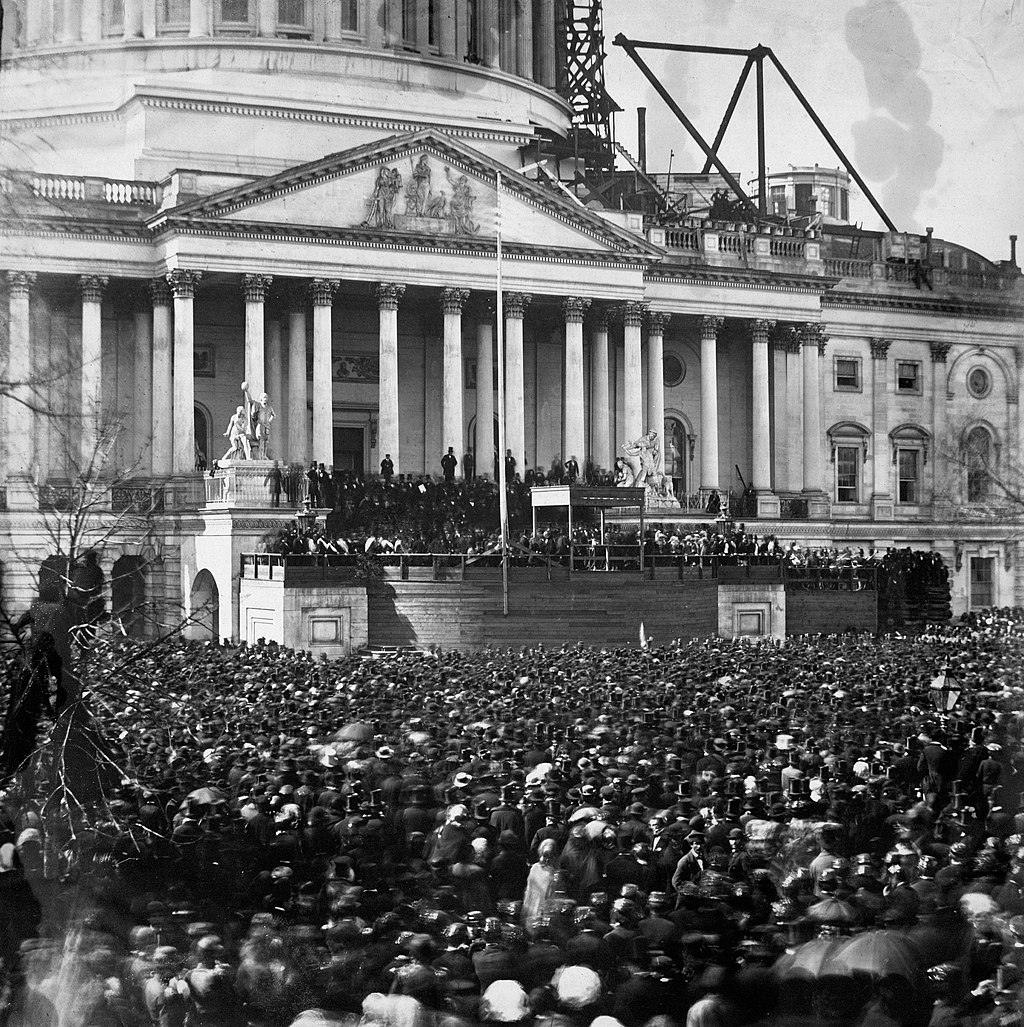
\includegraphics[width=5cm]{./img/inaugLincoln.jpg}\end{center}
The first inauguration of Abraham Lincoln as the 16th President of the United States was held on Monday, March 4, 1861, on the East Portico of the United States Capitol in Washington, D.C.. The inauguration marked the commencement of the first term of Abraham Lincoln as President and the only term of Hannibal Hamlin as Vice President. The presidential oath of office was administered to Lincoln by Roger B. Taney, Chief Justice of the United States.\\
This was the first time Lincoln appeared in public with a beard, which he had begun growing after being elected president, in response to a written request by 11-year-old Grace Bedell. This effectively made him the first President to have any facial hair beyond sideburns.\\
On Inauguration Day, Lincoln's procession to the Capitol was surrounded by heavily armed cavalry and infantry, providing an unprecedented amount of protection for the President-elect as the nation stood on the brink of war. During the 16 weeks between Lincoln's victory in the 1860 presidential election and Inauguration Day, seven slave states had declared their secession from the Union and formed the Confederate States of America.

\chapter{1865}
\section{May 12}
\subsection{Founding of Nokia}
\vspace{2mm}\begin{center}
\includegraphics[width=5cm]{./img/nokiaLogo.jpg}\end{center}
Nokia's history dates back to 1865, when Finnish-Swede mining engineer Fredrik Idestam established a pulp mill near the town of Tampere, Finland (then in the Russian Empire). A second pulp mill was opened in 1868 near the neighboring town of Nokia, offering better hydropower resources. In 1871, Idestam, together with friend Leo Mechelin, formed a shared company from it and called it Nokia Ab (in Swedish, Nokia Company being the English equivalent), after the site of the second pulp mill.\\
\indent Idestam retired in 1896, making Mechelin the company's chairman. Mechelin expanded into electricity generation by 1902 which Idestam had opposed. In 1904 Suomen Gummitehdas (Finnish Rubber Works), a rubber business founded by Eduard Polón, established a factory near the town of Nokia and used its name.\\ \indent In 1922, Nokia Ab entered into a partnership with Finnish Rubber Works and Kaapelitehdas (the Cable Factory), all now jointly under the leadership of Polón. Finnish Rubber Works company grew rapidly when it moved to the Nokia region in the 1930s to take advantage of the electrical power supply, and the cable company soon did too.\\
\indent Nokia at the time also made respirators for both civilian and military use, from the 1930s well into the early 1990s.

\chapter{1866}
\section{}
\subsection{Founding of Nestlé}
\vspace{2mm}\begin{center}
\includegraphics[width=5cm]{./img/nestleLogo.jpg}\end{center}
Nestlé's origins date back to the 1860s, when two separate Swiss enterprises were founded that would later form the core of Nestlé. In the succeeding decades, the two competing enterprises aggressively expanded their businesses throughout Europe and the United States.\\
\indent In 1866, Charles Page (US consul to Switzerland) and George Page, brothers from Lee County, Illinois, USA, established the Anglo-Swiss Condensed Milk Company in Cham, Switzerland. Their first British operation was opened at Chippenham, Wiltshire, in 1873.\\
\indent In 1867, in Vevey, Henri Nestlé developed milk-based baby food and soon began marketing it. The following year saw Daniel Peter begin seven years of work perfecting his invention, the milk chocolate manufacturing process. Nestlé was the crucial co-operation that Peter needed to solve the problem of removing all the water from the milk added to his chocolate and thus preventing the product from developing mildew. Henri Nestlé retired in 1875 but the company, under new ownership, retained his name as Société Farine Lactée Henri Nestlé.\\
\indent In 1877, Anglo-Swiss added milk-based baby foods to their products; in the following year, the Nestlé Company added condensed milk to their portfolio, which made the firms direct and fierce rivals.\\ \indent In 1879, Nestlé merged with milk chocolate inventor Daniel Peter.

\chapter{1869}
\section{October 02}
\subsection{Birth of Monhandas Gandhi}
\vspace{2mm}\begin{center}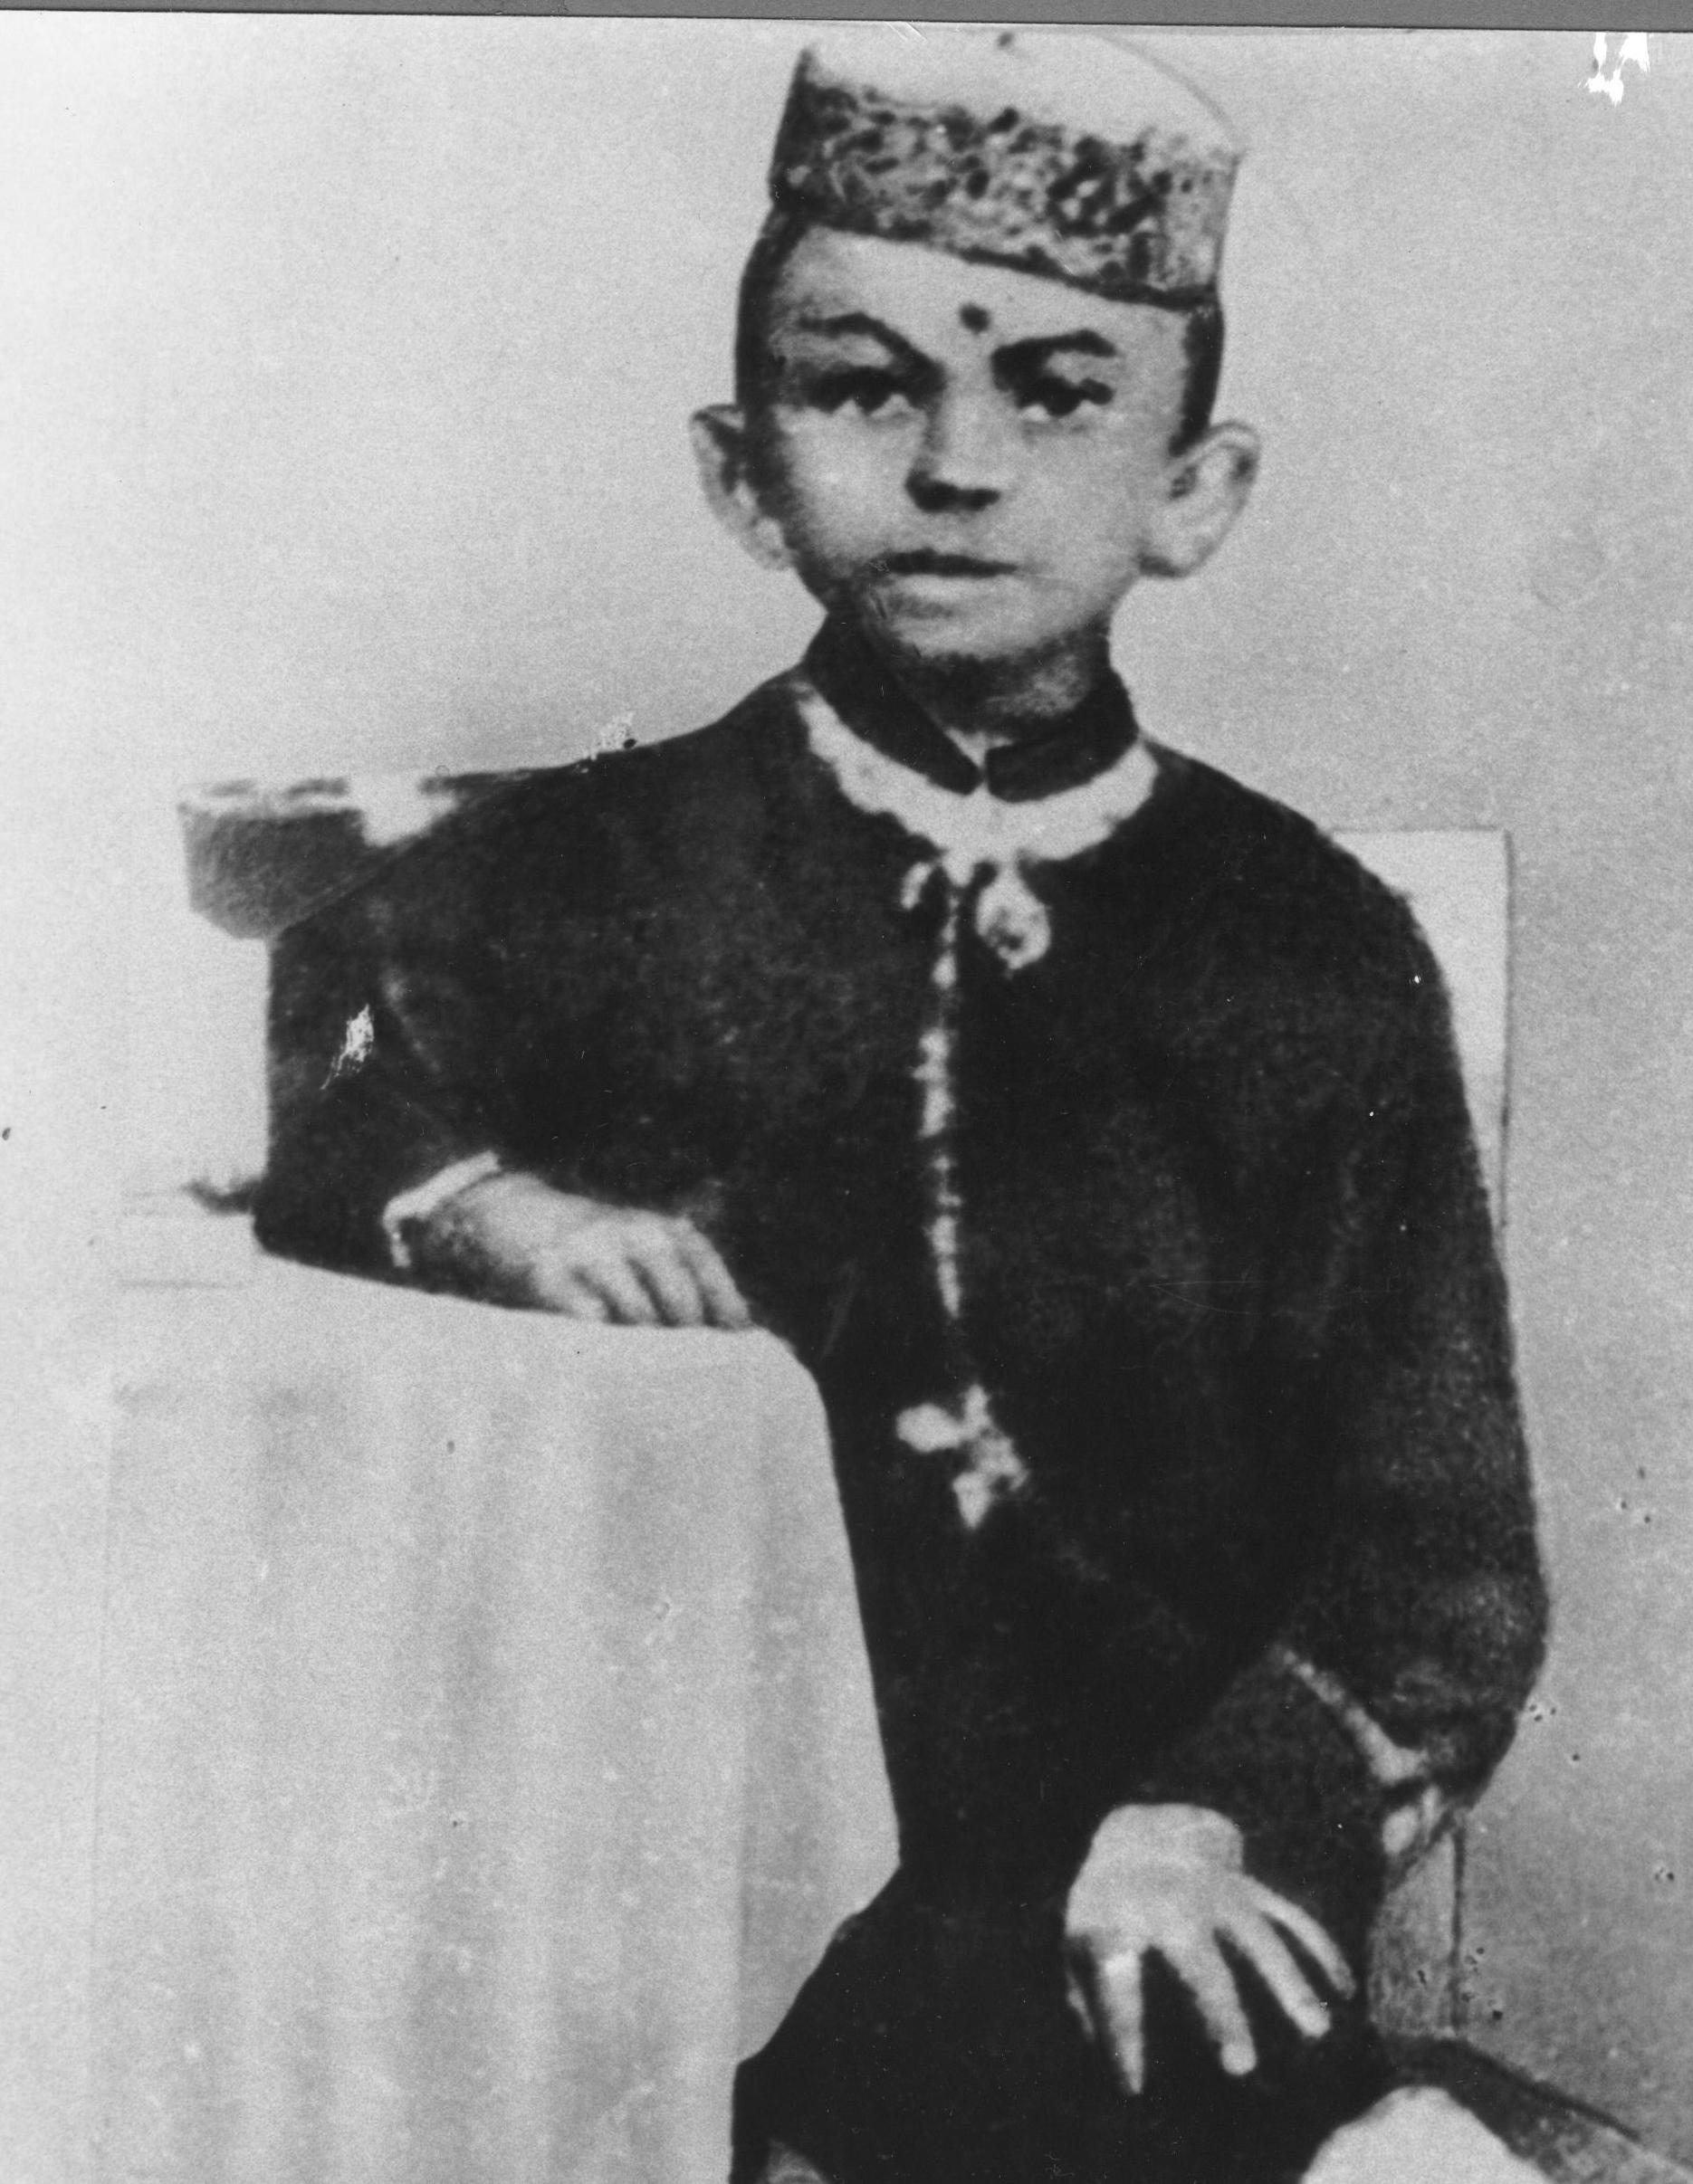
\includegraphics[width=5cm]{./img/youngGandhi.jpg}\end{center}
Mohandas Karamchand Gandhi was born on 2 October 1869 into a Gujarati Hindu Modh Baniya family in Porbandar (also known as Sudamapuri), a coastal town on the Kathiawar Peninsula and then part of the small princely state of Porbandar in the Kathiawar Agency of the Indian Empire. His father, Karamchand Uttamchand Gandhi (1822–1885), served as the diwan (chief minister) of Porbandar state.\\
Although he only had an elementary education and had previously been a clerk in the state administration, Karamchand proved a capable chief minister. During his tenure, Karamchand married four times. His first two wives died young, after each had given birth to a daughter, and his third marriage was childless. In 1857, Karamchand sought his third wife's permission to remarry; that year, he married Putlibai (1844–1891), who also came from Junagadh, and was from a Pranami Vaishnava family. Karamchand and Putlibai had three children over the ensuing decade: a son, Laxmidas (c. 1860–1914); a daughter, Raliatbehn (1862–1960); and another son, Karsandas (c. 1866–1913).

\chapter{1879}
\section{March 14}
\subsection{Birth of Albert Einstein}
\vspace{2mm}\begin{center}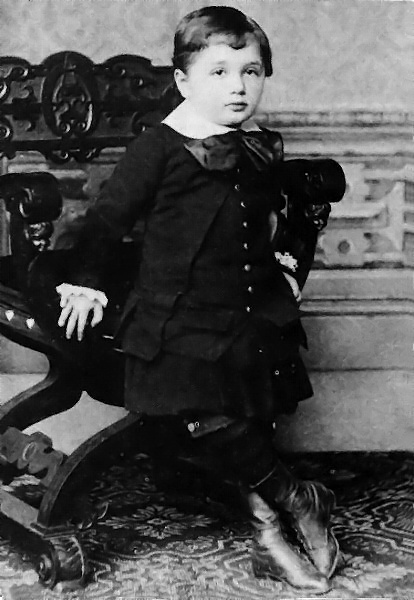
\includegraphics[width=6cm]{./img/youngEinstein.jpg}\end{center}
Albert Einstein was born in Ulm, in the Kingdom of Württemberg in the German Empire, on 14 March 1879. His parents were Hermann Einstein, a salesman and engineer, and Pauline Koch. In 1880, the family moved to Munich, where Einstein's father and his uncle Jakob founded Elektrotechnische Fabrik J. Einstein \& Cie, a company that manufactured electrical equipment based on direct current.\\
The Einsteins were non-observant Ashkenazi Jews, and Albert attended a Catholic elementary school in Munich, from the age of 5, for three years. At the age of 8, he was transferred to the Luitpold Gymnasium (now known as the Albert Einstein Gymnasium), where he received advanced primary and secondary school education until he left the German Empire seven years later.

\chapter{1886}
\section{May 08}
\subsection{Introduction of Coca-Cola}
\vspace{2mm}\begin{center}
\includegraphics[width=5cm]{./img/cocacolaLogo.jpg}\end{center}
Confederate Colonel John Pemberton, who was wounded in the American Civil War and became addicted to morphine, began a quest to find a substitute for the problematic drug. In 1885 at Pemberton's Eagle Drug and Chemical House, a drugstore in Columbus, Georgia, he registered Pemberton's French Wine Coca nerve tonic. Pemberton's tonic may have been inspired by the formidable success of Vin Mariani, a French-Corsican coca wine, but his recipe additionally included the African kola nut, the beverage's source of caffeine.\\ \indent It is also worth noting that a Spanish drink called "Kola Coca" was presented at a contest in Philadelphia in 1885, a year before the official birth of Coca-Cola. The rights for this Spanish drink were bought by Coca-Cola in 1953.\\ \indent In 1886, when Atlanta and Fulton County passed prohibition legislation, Pemberton responded by developing Coca-Cola, a nonalcoholic version of Pemberton's French Wine Coca. The first sales were at Jacob's Pharmacy in Atlanta, Georgia, on May 8, 1886, where it initially sold for five cents a glass. Drugstore soda fountains were popular in the United States at the time due to the belief that carbonated water was good for the health, and Pemberton's new drink was marketed and sold as a patent medicine, Pemberton claiming it a cure for many diseases, including morphine addiction, indigestion, nerve disorders, headaches, and impotence. Pemberton ran the first advertisement for the beverage on May 29 of the same year in the Atlanta Journal.

\chapter{1887}
\section{January 28}
\subsection{Beginning of Eiffel Tower construction}
\vspace{2mm}\begin{center}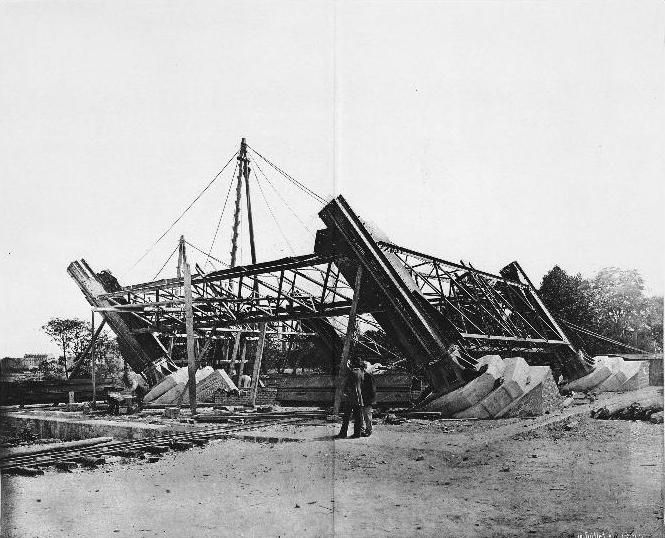
\includegraphics[width=10cm]{./img/eiffelTowerConstruction.jpg}\end{center}
Work on the foundations started on 28 January 1887. Those for the east and south legs were straightforward, with each leg resting on four 2 m (6.6 ft) concrete slabs, one for each of the principal girders of each leg. The west and north legs, being closer to the river Seine, were more complicated: each slab needed two piles installed by using compressed-air caissons 15 m (49 ft) long and 6 m (20 ft) in diameter driven to a depth of 22 m (72 ft) to support the concrete slabs, which were 6 m (20 ft) thick. Each of these slabs supported a block of limestone with an inclined top to bear a supporting shoe for the ironwork.

\chapter{1889}
\section{April 16}
\subsection{Birth of Charles Chaplin}
\vspace{2mm}\begin{center}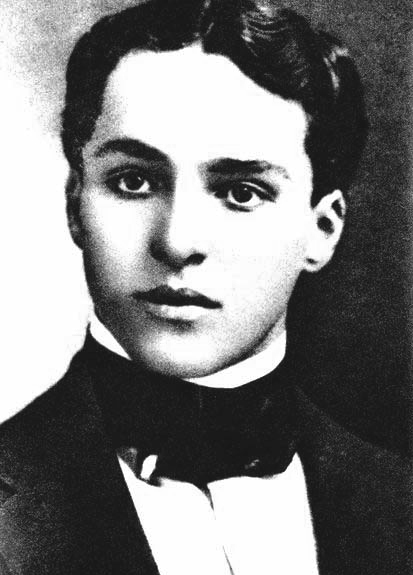
\includegraphics[width=5cm]{./img/youngchaplin.jpg}\end{center}
Charles Spencer Chaplin was born on 16 April 1889 to Hannah Chaplin (born Hannah Harriet Pedlingham Hill) and Charles Chaplin Sr. There is no official record of his birth, although Chaplin believed he was born at East Street, Walworth, in South London. His mother and father had married four years previously, at which time Charles Sr. became the legal guardian of Hannah's illegitimate son, Sydney John Hill. At the time of his birth, Chaplin's parents were both music hall entertainers. Hannah, the daughter of a shoemaker, had a brief and unsuccessful career under the stage name Lily Harley, while Charles Sr., a butcher's son, was a popular singer. Although they never divorced, Chaplin's parents were estranged by around 1891. The following year, Hannah gave birth to a third son – George Wheeler Dryden – fathered by the music hall entertainer Leo Dryden. The child was taken by Dryden at six months old, and did not re-enter Chaplin's life for 30 years.
\section{April 20}
\subsection{Birth of Adolf Hitler}
\vspace{2mm}\begin{center}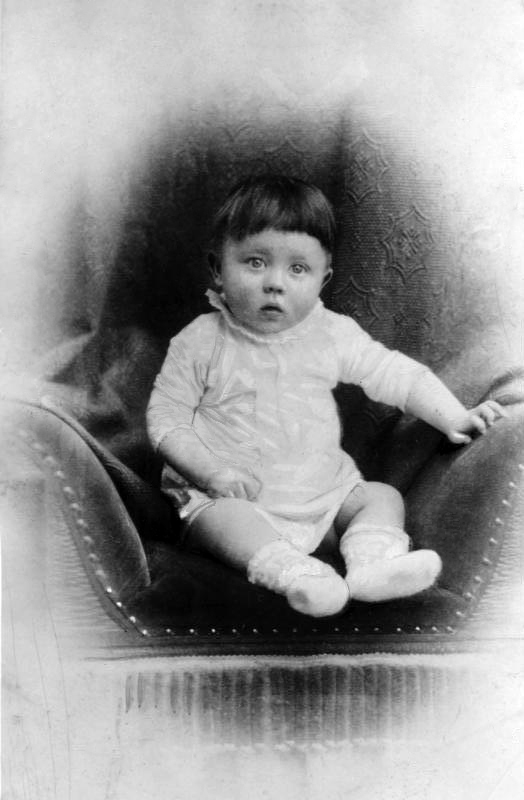
\includegraphics[width=5cm]{./img/infantHitler.jpg}\end{center}
Adolf Hitler was born on 20 April 1889 in Braunau am Inn, a town in Austria-Hungary (in present-day Austria), close to the border with the German Empire. He was christened as "Adolphus Hitler". He was the fourth of six children born to Alois Hitler and his third wife, Klara Pölzl. Three of Hitler's siblings—Gustav, Ida, and Otto—died in infancy. Also living in the household were Alois's children from his second marriage: Alois Jr. (born 1882) and Angela (born 1883). When Hitler was three, the family moved to Passau, Germany. There he acquired the distinctive lower Bavarian dialect, rather than Austrian German, which marked his speech throughout his life. The family returned to Austria and settled in Leonding in 1894, and in June 1895 Alois retired to Hafeld, near Lambach, where he farmed and kept bees. Hitler attended Volksschule (a state-owned primary school) in nearby Fischlham.
\section{September 23}
\subsection{Founding of Nintendo}
Nintendo was founded as a playing card company by Fusajiro Yamauchi on 23 September 1889. Based in Kyoto, the business produced and marketed Hanafuda cards. The handmade cards soon became popular, and Yamauchi hired assistants to mass-produce cards to satisfy demand. In 1949, the company adopted the name Nintendo Karuta Co., Ltd., doing business as The Nintendo Playing Card Co. outside Japan. Nintendo continues to manufacture playing cards in Japan and organises its own contract bridge tournament called the "Nintendo Cup". The word Nintendo can be translated as "leave luck to heaven", or alternatively as "the temple of free hanafuda".\\
\indent In 1956, Hiroshi Yamauchi, grandson of Fusajiro Yamauchi, visited the U.S. to talk with the United States Playing Card Company, the dominant playing card manufacturer there. He found that the biggest playing card company in the world was using only a small office. Yamauchi's realization that the playing card business had limited potential was a turning point. He then acquired the license to use Disney characters on playing cards to drive sales.\\
\indent In 1963, Yamauchi renamed Nintendo Playing Card Co. Ltd. to Nintendo Co., Ltd. The company then began to experiment in other areas of business using newly injected capital during the period of time between 1963 and 1968. Nintendo set up a taxi company called Daiya. This business was initially successful. However, Nintendo was forced to sell it because problems with the labour unions were making it too expensive to run the service. It also set up a love hotel chain, a TV network, a food company (selling instant rice) and several other ventures. All of these ventures eventually failed, and after the 1964 Tokyo Olympics, playing card sales dropped, and Nintendo's stock price plummeted to its lowest recorded level of ¥60.

\chapter{1892}
\section{January 03}
\subsection{Birth of J.R.R Tolkien}
\vspace{2mm}\begin{center}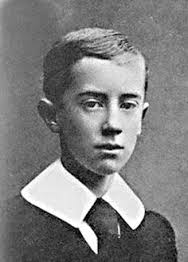
\includegraphics[width=5cm]{./img/youngTolkien.jpg}\end{center}
John Ronald Reuel Tolkien, (3 January 1892 – 2 September 1973) was an English writer, poet, philologist, and university professor who is best known as the author of the classic high fantasy works The Hobbit, The Lord of the Rings, and The Silmarillion.\\
He served as the Rawlinson and Bosworth Professor of Anglo-Saxon and Fellow of Pembroke College, Oxford, from 1925 to 1945 and Merton Professor of English Language and Literature and Fellow of Merton College, Oxford, from 1945 to 1959. He was at one time a close friend of C. S. Lewis, they were both members of the informal literary discussion group known as the Inklings. Tolkien was appointed a Commander of the Order of the British Empire by Queen Elizabeth II on 28 March 1972.

\chapter{1896}
\section{April 06-15}
\subsection{First international Olympic Games}
\vspace{2mm}\begin{center}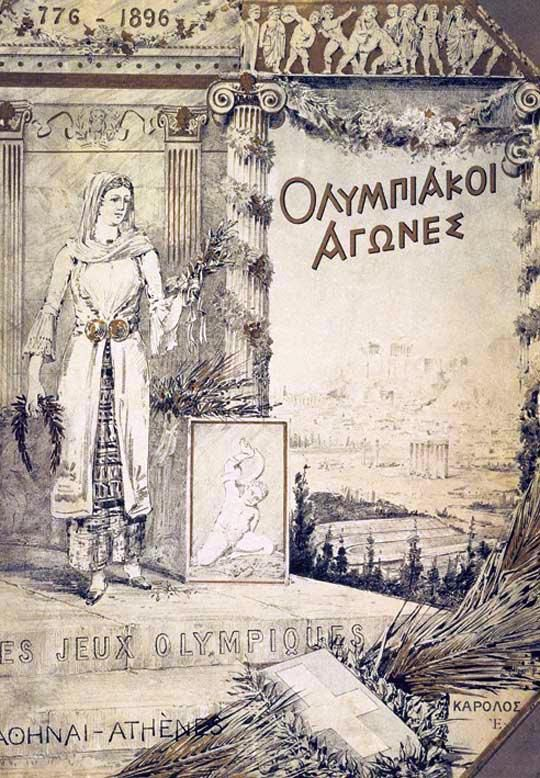
\includegraphics[width=5cm]{./img/olgames.jpg}\end{center}
The 1896 Summer Olympics officially known as the Games of the I Olympiad, was the first international Olympic Games held in modern history. Organised by the International Olympic Committee (IOC), which had been created by Pierre de Coubertin, it was held in Athens, Greece, from 6 to 15 April 1896.\\
Winners were given a silver medal, while runners-up received a copper medal. Retroactively, the IOC has converted these to gold and silver, and awarded bronze medals to third placed athletes. Ten of the 14 participating nations earned medals. The United States won the most gold medals, 11, host nation Greece won the most medals overall, 46. The highlight for the Greeks was the marathon victory by their compatriot Spyridon Louis. The most successful competitor was German wrestler and gymnast Carl Schuhmann, who won four events.

%             					20th century	
					
\part{20th Century}
\chapter{1900}
\section{-}
\subsection{Founding of Dodge}
\vspace{2mm}\begin{center}
\includegraphics[width=10cm]{./img/dodgeLogo.jpg}\end{center}
Horace and John Dodge founded the Dodge Brothers Company in Detroit in 1900, and quickly found work manufacturing precision engine and chassis components for the city's growing number of automobile firms. Chief among these customers were the established Olds Motor Vehicle Company and the new Ford Motor Company. Henry Ford selected the Dodge brothers to supply a wide range of components for his original Model A (1903–04) that included the complete chassis; thus Ford needed to add only the body and wheels to finish the cars.\\ \indent The first machine shop where the brothers worked as parts suppliers for Olds and Ford was located at the Boydell Building on Beaubien Street at Lafayette. This location was replaced by a larger facility at Hastings Street and Monroe Avenue, which is now a parking garage for the Greektown Casino Hotel (Hastings Street at this location has been renamed Chrysler Service Drive). By 1910 the Dodge Main factory was built in Hamtramck, where it remained until 1979.

\chapter{1903}
\section{June 16}
\subsection{Founding of Ford}
\vspace{2mm}\begin{center}
\includegraphics[width=7cm]{./img/fordLogo.jpg}\end{center}
Henry Ford's first attempt at a car company under his own name was the Henry Ford Company on November 3, 1901, which became the Cadillac Motor Company on August 22, 1902, after Ford left with the rights to his name. The Ford Motor Company was launched in a converted factory in 1903 with \$28,000 in cash from twelve investors, most notably John and Horace Dodge (who would later found their own car company). The first president was not Ford, but local banker John S. Gray, who was chosen to assuage investors' fears that Ford would leave the new company the way he had left its predecessor. During its early years, the company produced just a few cars a day at its factory on Mack Avenue and later its factory on Piquette Avenue in Detroit, Michigan. Groups of two or three men worked on each car, assembling it from parts made mostly by supplier companies contracting for Ford. Within a decade, the company would lead the world in the expansion and refinement of the assembly line concept, and Ford soon brought much of the part production in-house in a vertical integration that seemed a better path for the era.
\section{December 17}
\subsection{First flight by the Wright brothers}
\vspace{2mm}\begin{center}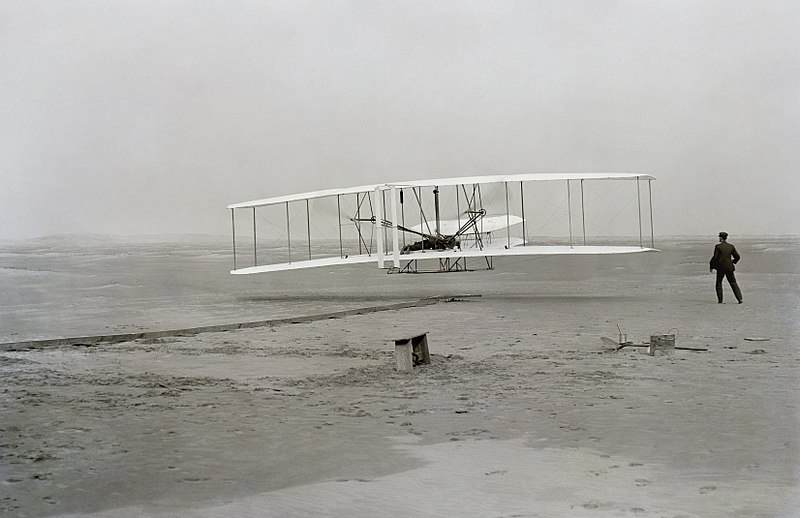
\includegraphics[width=10cm]{./img/firstflight.jpg}\end{center}
In camp at Kill Devil Hills, they endured weeks of delays caused by broken propeller shafts during engine tests. After the shafts were replaced (requiring two trips back to Dayton), Wilbur won a coin toss and made a three-second flight attempt on December 14, 1903, stalling after takeoff and causing minor damage to the Flyer. (Because December 13, 1903, was a Sunday, the brothers did not make any attempts that day, even though the weather was good, so their first powered test flight happened on the 121st anniversary of the first test flight that the Montgolfier brothers had done, on December 14, 1782.) In a message to their family, Wilbur referred to the trial as having "only partial success", stating "the power is ample, and but for a trifling error due to lack of experience with this machine and this method of starting, the machine would undoubtedly have flown beautifully." Following repairs, the Wrights finally took to the air on December 17, 1903, making two flights each from level ground into a freezing headwind gusting to 27 miles per hour (43 km/h). The first flight, by Orville at 10:35 am, of 120 feet (37 m) in 12 seconds, at a speed of only 6.8 miles per hour (10.9 km/h) over the ground, was recorded in a famous photograph. The next two flights covered approximately 175 and 200 feet (53 and 61 m), by Wilbur and Orville respectively. Their altitude was about 10 feet (3.0 m) above the ground. The following is Orville Wright's account of the final flight of the day.
\section{-}
\subsection{Founding of Harley-Davidson}
\vspace{2mm}\begin{center}
\includegraphics[width=5cm]{./img/harleyDavidsonLogo.jpg}\end{center}
In 1901, 20-year-old William S. Harley drew up plans for a small engine with a displacement of 7.07 cubic inches (116 cc) and four-inch (102 mm) flywheels. The engine was designed for use in a regular pedal-bicycle frame. Over the next two years, Harley and his childhood friend Arthur Davidson worked on their motor-bicycle using the northside Milwaukee machine shop at the home of their friend, Henry Melk. It was finished in 1903 with the help of Arthur's brother, Walter Davidson. Upon testing their power-cycle, Harley and the Davidson brothers found it unable to climb the hills around Milwaukee without pedal assistance. They quickly wrote off their first motor-bicycle as a valuable learning experiment.\\ \indent Work immediately began on a new and improved second-generation machine. This first "real" Harley-Davidson motorcycle had a bigger engine of 24.74 cubic inches (405 cc) with 9.75 inches (25 cm) flywheels weighing 28 lb (13 kg). The machine's advanced loop-frame pattern was similar to the 1903 Milwaukee Merkel motorcycle (designed by Joseph Merkel, later of Flying Merkel fame). The bigger engine and loop-frame design took it out of the motorized bicycle category and marked the path to future motorcycle designs. The boys also received help with their bigger engine from outboard motor pioneer Ole Evinrude, who was then building gas engines of his own design for automotive use on Milwaukee's Lake Street.

\chapter{1904}
\section{May 21}
\subsection{Founding of FIFA}
\vspace{2mm}\begin{center}
\includegraphics[width=5cm]{./img/fifaLogo.jpg}\end{center}
The need for a single body to oversee association football became apparent at the beginning of the 20th century with the increasing popularity of international fixtures. The Fédération Internationale de Football Association (FIFA) was founded in the rear of the headquarters of the Union des Sociétés Françaises de Sports Athlétiques (USFSA) at the Rue Saint Honoré 229 in Paris on 21 May 1904. The French name and acronym are used even outside French-speaking countries. The founding members were the national associations of Belgium, Denmark, France, the Netherlands, Spain (represented by the then-Madrid Football Club; the Royal Spanish Football Federation was not created until 1913), Sweden and Switzerland. Also, that same day, the German Football Association (DFB) declared its intention of affiliating through a telegram.\\
\indent The first president of FIFA was Robert Guérin. Guérin was replaced in 1906 by Daniel Burley Woolfall from England, by then a member of the association. The first tournament FIFA staged, the association football competition for the 1908 Olympics in London was more successful than its Olympic predecessors, despite the presence of professional footballers, contrary to the founding principles of FIFA.\\ \indent Membership of FIFA expanded beyond Europe with the application of South Africa in 1909, Argentina in 1912, Canada and Chile in 1913, and the United States in 1914.

\chapter{1905}
\section{-}
\subsection{Founding of Rolex}
\vspace{2mm}\begin{center}\includegraphics[width=5cm]{./img/rolexLogo.jpg}\end{center}
Alfred Davis and his brother-in-law Hans Wilsdorf founded Wilsdorf and Davis, the company that would eventually become Rolex SA, in London, England in 1905. Wilsdorf and Davis' main commercial activity at the time involved importing Hermann Aegler's Swiss movements to England and placing them in watch cases made by Dennison and others. These early wristwatches were sold to many jewellers, who then put their own names on the dial. The earliest watches from Wilsdorf and Davis were usually hallmarked "W\&D" inside the caseback.\\
\indent In 1908 Wilsdorf registered the trademark "Rolex" and opened an office in La Chaux-de-Fonds, Switzerland. The company name "Rolex" was registered on 15 November 1915. The book The Best of Time: Rolex Wristwatches: An Unauthorized History by Jeffrey P. Hess and James Dowling says that the name was just made up. One story, never confirmed by Wilsdorf, recounts that the name came from the French phrase horlogerie exquise, meaning "exquisite clockwork" or as a contraction of "horological excellence". Wilsdorf was said to want his watch brand's name to be easily pronounceable in any language. He also thought that the name "Rolex" was onomatopoeic, sounding like a watch being wound. It is easily pronounceable in many languages and, as all its upper-case letters have the same size, can be written symmetrically. It was also short enough to fit on the face of a watch

\chapter{1906}
\section{February 19}
\subsection{Introduction of Kellogg's}
\vspace{2mm}\begin{center}\includegraphics[width=5cm]{./img/kelloggsLogo.jpg}\end{center}
Brothers Dr. John Harvey and Will Keith Kellogg founded a health food company, the Battle Creek Sanitarium Health Food Company in 1898. This company produced foodstuffs for current and former patients at Dr. J. H. Kellogg's Battle Creek Sanitarium. The company later became known as the Battle Creek Sanitarium Food Company in 1901. During this time, the company produced and marketed health foods such as corn flakes, Granola and Caramel Cereal Coffee.\\ \indent The company merged with the Sanitas Nut Food Company (founded in 1899 by Dr. J. H. Kellogg) to become the Kellogg Food Company in July 1908, and sold nut butters and meat substitutes, and it was then that the company's products all began to be sold under the trade name, "Kellogg's". At this time, Dr. J. H. Kellogg owned all but 2 of its 15,000 shares of stock. In 1921, it changed its name back to Battle Creek Food Company.\\
\indent In 1930, the Kellogg Company announced that most of its factories would shift towards 30-hour work weeks, from the usual 40. W.K. Kellogg stated that he did this so that an additional shift of workers would be employed in an effort to support people through the depression era. This practice remained until World War II, and continued briefly after the war, although some departments and factories remained locked into 30-hour work weeks until 1980.

\chapter{1907}
\section{August 31}
\subsection{Creation of the Triple Entente}
\vspace{2mm}\begin{center}\includegraphics[width=5cm]{./img/tripleEntente.jpg}\end{center}
The Triple Entente refers to the understanding linking the Russian Empire, the French Third Republic, and United Kingdom of Great Britain and Ireland after the signing of the Anglo-Russian Entente on 31 August 1907. The understanding between the three powers, supplemented by agreements with Japan and Portugal, was a powerful counterweight to the Triple Alliance of Germany, Austria-Hungary, and Italy.\\
However, Italy did not side with Germany and Austria during World War I and joined the Entente instead in the Treaty of London (1915).\\
Historians continue to debate the importance of the alliance system as one of the causes of World War I. At the start of World War I in 1914, all three Triple Entente members entered it as Allied Powers against the Central Powers: Germany and Austria-Hungary.\\
However, the Triple Entente, unlike the Triple Alliance or the Franco-Russian Alliance, was not an alliance of mutual defense. Thus, Britain felt free to make its own foreign policy decisions in the 1914 July Crisis.

\chapter{1908}
\section{July 16}
\subsection{Formation of the FBI}
\vspace{2mm}\begin{center}\includegraphics[width=5cm]{./img/FBILogo.jpg}\end{center}
The Bureau of Investigation (BOI) was created on July 26, 1908, after the Congress had adjourned for the summer. Attorney General Bonaparte, using Department of Justice expense funds, hired thirty-four people, including some veterans of the Secret Service, to work for a new investigative agency. Its first "Chief" (the title is now known as "Director") was Stanley Finch. Bonaparte notified the Congress of these actions in December 1908.\\
The bureau's first official task was visiting and making surveys of the houses of prostitution in preparation for enforcing the "White Slave Traffic Act," or Mann Act, passed on June 25, 1910. In 1932, the bureau was renamed the United States Bureau of Investigation. The following year it was linked to the Bureau of Prohibition and rechristened the Division of Investigation (DOI) before finally becoming an independent service within the Department of Justice in 1935. In the same year, its name was officially changed from the Division of Investigation to the present-day Federal Bureau of Investigation, or FBI.

\chapter{1909}
\section{-}
\subsection{Founding of Buggati}
\vspace{2mm}\begin{center}\includegraphics[width=5cm]{./img/bugattiLogo.jpg}\end{center}
Founder Ettore Bugatti was born in Milan, Italy, and the automobile company that bears his name was founded in 1909 in Molsheim located in the Alsace region which was part of the German Empire from 1871 to 1919. The company was known both for the level of detail of its engineering in its automobiles, and for the artistic manner in which the designs were executed, given the artistic nature of Ettore's family (his father, Carlo Bugatti (1856–1940), was an important Art Nouveau furniture and jewelry designer).\\ \indent During the war Ettore Bugatti was sent away, initially to Milan and later to Paris, but as soon as hostilities had been concluded he returned to his factory at Molsheim. Less than four months after the Versailles Treaty formalised the transfer of Alsace from Germany to France, Bugatti was able to obtain, at the last minute, a stand at the 15th Paris motor show in October 1919. He exhibited three light cars, all of them closely based on their pre-war equivalents, and each fitted with the same overhead camshaft 4-cylinder 1,368cc engine with four valves per cylinder. Smallest of the three was a "Type 13" with a racing body (constructed by Bugatti themselves) and using a chassis with a 2,000 mm (78.7 in) wheelbase. The others were a "Type 22" and a "Type 23" with wheelbases of 2,250 and 2,400 mm (88.6 and 94.5 in) respectively.
\subsection{Founding of Suzuki}
Suzuki Motor Corporation is a Japanese multinational corporation headquartered in Minami-ku, Hamamatsu. Suzuki manufactures automobiles, four-wheel drive vehicles, motorcycles, all-terrain vehicles (ATVs), outboard marine engines, wheelchairs and a variety of other small internal combustion engines. In 2016, Suzuki was the eleventh biggest automaker by production worldwide. Suzuki has over 45,000 employees and has 35 production facilities in 23 countries, and 133 distributors in 192 countries. The worldwide sales volume of automobiles is the world's tenth largest, while domestic sales volume is the third largest in the country.\\ \indent In 1909, Michio Suzuki (1887–1982) founded the Suzuki Loom Works in the small seacoast village of Hamamatsu, Japan. Business boomed as Suzuki built weaving looms for Japan's giant silk industry. In 1929, Michio Suzuki invented a new type of weaving machine, which was exported overseas. The company's first 30 years focused on the development and production of these machines.\\ \indent Despite the success of his looms, Suzuki believed that his company would benefit from diversification and he began to look at other products. Based on consumer demand, he decided that building a small car would be the most practical new venture. The project began in 1937, and within two years Suzuki had completed several compact prototype cars. These first Suzuki motor vehicles were powered by a then-innovative, liquid-cooled, four-stroke, four-cylinder engine. It had a cast aluminum crankcase and gearbox and generated 13 horsepower (9.7 kW) from a displacement of less than 800cc.

\chapter{1910}
\section{April 25}
\subsection{Founding of Audi}
Audi AG is a German automobile manufacturer that designs, engineers, produces, markets and distributes luxury vehicles. Audi is a member of the Volkswagen Group and has its roots at Ingolstadt, Bavaria, Germany. Audi-branded vehicles are produced in nine production facilities worldwide. Automobile company Wanderer was originally established in 1885, later becoming a branch of Audi AG. Another company, NSU, which also later merged into Audi, was founded during this time, and later supplied the chassis for Gottlieb Daimler's four-wheeler.\ On 14 November 1899, August Horch (1868–1951) established the company A. Horch \& Cie. in the Ehrenfeld district of Cologne. In 1902, he moved with his company to Reichenbach im Vogtland. On 10 May 1904, he founded the August Horch \& Cie. Motorwagenwerke AG, a joint-stock company in Zwickau (State of Saxony).\\ \indent Since August Horch was prohibited from using "Horch" as a trade name in his new car business, he called a meeting with close business friends, Paul and Franz Fikentscher from Zwickau. At the apartment of Franz Fikentscher, they discussed how to come up with a new name for the company. During this meeting, Franz's son was quietly studying Latin in a corner of the room. Several times he looked like he was on the verge of saying something but would just swallow his words and continue working, until he finally blurted out, "Father – audiatur et altera pars... wouldn't it be a good idea to call it audi instead of horch?" "Horch!" in German means "Hark!" or "hear", which is "Audi" in the singular imperative form of "audire" – "to listen" – in Latin. The idea was enthusiastically accepted by everyone attending the meeting. On 25 April 1910 the Audi Automobilwerke GmbH Zwickau (from 1915 on Audiwerke AG Zwickau) was entered in the company's register of Zwickau registration court.

\chapter{1911}
\section{June 16}
\subsection{Founding of IBM}
In the 1880s, technologies emerged that would ultimately form the core of International Business Machines (IBM). Julius E. Pitrap patented the computing scale in 1885; Alexander Dey invented the dial recorder (1888); Herman Hollerith (1860–1929) patented the Electric Tabulating Machine; and Willard Bundy invented a time clock to record a worker's arrival and departure time on a paper tape in 1889. On June 16, 1911, their four companies were amalgamated in New York State by Charles Ranlett Flint forming a fifth company, the Computing-Tabulating-Recording Company (CTR) based in Endicott, New York. The five companies had 1,300 employees and offices and plants in Endicott and Binghamton, New York; Dayton, Ohio; Detroit, Michigan; Washington, D.C.; and Toronto.\\ \indent They manufactured machinery for sale and lease, ranging from commercial scales and industrial time recorders, meat and cheese slicers, to tabulators and punched cards. Thomas J. Watson, Sr., fired from the National Cash Register Company by John Henry Patterson, called on Flint and, in 1914, was offered a position at CTR. Watson joined CTR as General Manager then, 11 months later, was made President when court cases relating to his time at NCR were resolved. Having learned Patterson's pioneering business practices, Watson proceeded to put the stamp of NCR onto CTR's companies. He implemented sales conventions, "generous sales incentives, a focus on customer service, an insistence on well-groomed, dark-suited salesmen and had an evangelical fervor for instilling company pride and loyalty in every worker". His favorite slogan, "THINK", became a mantra for each company's employees. During Watson's first four years, revenues reached \$9 million and the company's operations expanded to Europe, South America, Asia and Australia. Watson never liked the clumsy hyphenated name "Computing-Tabulating-Recording Company" and on February 14, 1924 chose to replace it with the more expansive title "International Business Machines". By 1933 most of the subsidiaries had been merged into one company, IBM.

\chapter{1912}
\section{April 14-15}
\subsection{Sinking of the RMS Titanic}
\vspace{2mm}\begin{center}\includegraphics[width=5cm]{./img/titanicsinking.jpg}\end{center}
RMS Titanic sank in the early morning of 15 April 1912 in the North Atlantic Ocean, four days into the ship's maiden voyage from Southampton to New York City. The largest passenger liner in service at the time, Titanic had an estimated 2,224 people on board when she struck an iceberg at around 23:40 (ship's time) on Sunday, 14 April 1912. Her sinking two hours and forty minutes later at 02:20 (ship's time; 05:18 GMT) on Monday, 15 April, resulted in the deaths of more than 1,500 people, which made it one of the deadliest peacetime maritime disasters in history.\\
On 14 April 1912, Titanic's radio operators received six messages from other ships warning of drifting ice, which passengers on Titanic had begun to notice during the afternoon. The ice conditions in the North Atlantic were the worst for any April in the previous 50 years (which was the reason why the lookouts were unaware that they were about to steam into a line of drifting ice several miles wide and many miles long). Not all of these messages were relayed by the radio operators. At the time, all wireless operators on ocean liners were employees of the Marconi's Wireless Telegraph Company and not members of their ship's crew; their primary responsibility was to send messages for the passengers, with weather reports as a secondary concern.

\chapter{1914}
\section{June 28}
\subsection{Assassination of Franz Ferdinand\protect\footnote{Movie/History: Sarajevo (2014)}}
\vspace{2mm}\begin{center}\includegraphics[width=5cm]{./img/franzFerdinand.jpg}\end{center}
The assassination of Archduke Franz Ferdinand of Austria, heir presumptive to the Austro-Hungarian throne, and his wife Sophie, Duchess of Hohenberg, occurred on 28 June 1914 in Sarajevo when they were mortally wounded by Gavrilo Princip. Princip was one of a group of six assassins (five Serbs and one Bosniak) coordinated by Danilo Ilić, a Bosnian Serb and a member of the Black Hand secret society. The political objective of the assassination was to break off Austria-Hungary's South Slav provinces so they could be combined into a Yugoslavia. The assassins' motives were consistent with the movement that later became known as Young Bosnia. The assassination led directly to the First World War when Austria-Hungary subsequently issued an ultimatum to the Kingdom of Serbia, which was partially rejected. Austria-Hungary then declared war, triggering actions leading to war between most European states.
\section{July 28}
\subsection{Austria-Hungary declares war on Serbia (World War I\protect\footnote{Documentary: They Shall Not Grow Old (2018)} begins)}
\vspace{2mm}\begin{center}\includegraphics[width=10cm]{./img/austriaWarSerbia.jpg}\end{center}
On July 28, 1914, one month to the day after Archduke Franz Ferdinand of Austria and his wife were killed by a Serbian nationalist in Sarajevo, Austria-Hungary declares war on Serbia, effectively beginning the First World War.\\
Threatened by Serbian ambition in the tumultuous Balkans region of Europe, Austria-Hungary determined that the proper response to the assassinations was to prepare for a possible military invasion of Serbia. After securing the unconditional support of its powerful ally, Germany, Austria-Hungary presented Serbia with a rigid ultimatum on July 23, 1914, demanding, among other things, that all anti-Austrian propaganda within Serbia be suppressed, and that Austria-Hungary be allowed to conduct its own investigation into the archduke’s killing. Though Serbia effectively accepted all of Austria’s demands except for one, the Austrian government broke diplomatic relations with the other country on July 25 and went ahead with military preparedness measures. Meanwhile, alerted to the impending crisis, Russia—Serbia’s own mighty supporter in the Balkans—began its own initial steps towards military mobilization against Austria.
\section{July 31}
\subsection{Russia mobilizes its army in defense of Serbia}
Reacting to the Austrian attack on Serbia, Russia begins full mobilization of its troops. Germany demands that it stop.
\section{August 01}
\subsection{Germany declares war on Russia}
Germany declares war on Russia. France and Belgium begin full mobilization.
\section{August 03}
\subsection{Germany declares war on France}
Germany declares war on France, and invades neutral Belgium. Britain then sends an ultimatum, rejected by the Germans, to withdraw from Belgium.
\section{August 04}
\subsection{Germany invades neutral Belgium}
\vspace{2mm}\begin{center}\includegraphics[width=12cm]{./img/germanyInBelgium.jpg}\end{center}
The German invasion of Belgium was a military campaign which began on 4 August 1914. Earlier, on 24 July, the Belgian government had announced that if war came it would uphold its historic neutrality. The Belgian government mobilised its armed forces on 31 July and a state of heightened alert (Kriegsgefahr) was proclaimed in Germany. On 2 August, the German government sent an ultimatum to Belgium, demanding passage through the country and German forces invaded Luxembourg. Two days later, the Belgian Government refused the demands and the British Government guaranteed military support to Belgium. The German government declared war on Belgium on 4 August, troops crossed the border and began the Battle of Liège.
\section{August 05}
\subsection{Battle of Liège}
\vspace{2mm}\begin{center}\includegraphics[width=12cm]{./img/battleOfLiege.jpg}\end{center}
The Battle of Liège (French: Bataille de Liège) was the opening engagement of the German invasion of Belgium and the first battle of the First World War. The attack on Liège, a town protected by the Fortified position of Liège, a ring fortress built from the late 1880s to the early 1890s, began on 5 August 1914 and lasted until 16 August, when the last fort surrendered. The siege of Liège may have delayed the German invasion of France by 4–5 days. Railways in the Meuse river valley needed by the German armies in eastern Belgium were closed for the duration of the siege and German troops did not appear in strength before the Fortified Position of Namur at the confluence of the Sambre and Meuse rivers until 20 August.
\section{August 15-24}
\subsection{Battle of Cer}
\vspace{2mm}\begin{center}\includegraphics[width=8cm]{./img/battleOfCer.jpg}\end{center}
The Battle of Cer was a military campaign fought between Austria-Hungary and Serbia in August 1914 during the early stages of the Serbian Campaign of the First World War. It took place around Cer Mountain and several surrounding villages, as well as the town of Šabac.\\
The battle, part of the first Austro-Hungarian invasion of Serbia, began on the night of 15 August when elements of the Serbian 1st Combined Division encountered Austro-Hungarian outposts that had been established on the slopes of Cer Mountain earlier in the invasion. The clashes that followed escalated into a battle for control over several towns and villages near the mountain, especially Šabac. On 19 August, the morale of the Austro-Hungarians collapsed and thousands of soldiers retreated back into Austria-Hungary, many of them drowning in the Drina River as they fled in panic. On 24 August the Serbs re-entered Šabac, marking the end of the battle. Serbian casualties after nearly ten days of fighting were 3,000–5,000 killed and 15,000 wounded. Those of the Austro-Hungarians were significantly higher, with 6,000–10,000 soldiers killed, 30,000 wounded and 4,500 taken as prisoners of war. The Serb victory over the Austro-Hungarians marked the first Allied victory over the Central Powers in the First World War, and the first aerial dogfight of the war took place during the battle.
\section{August-September}
\subsection{Battle of Galicia}
\vspace{2mm}\begin{center}\includegraphics[width=10cm]{./img/battleOfGalicia.jpg}\end{center}
The Battle of Galicia, also known as the Battle of Lemberg, was a major battle between Russia and Austria-Hungary during the early stages of World War I in 1914. In the course of the battle, the Austro-Hungarian armies were severely defeated and forced out of Galicia, while the Russians captured Lemberg and, for approximately nine months, ruled Eastern Galicia until their defeat at Gorlice and Tarnów.
\subsection{Battle of Frontiers}
\vspace{2mm}\begin{center}\includegraphics[width=10cm]{./img/battleOfFrontier.jpg}\end{center}
The Battle of the Frontiers (Dutch: Slag der Grenzen; French: Bataille des Frontières; German: Grenzschlachten) was a series of battles fought along the eastern frontier of France and in southern Belgium, shortly after the outbreak of the First World War. The battles resolved the military strategies of the French Chief of Staff General Joseph Joffre with Plan XVII and an offensive interpretation of the German Aufmarsch II deployment plan by Helmuth von Moltke the Younger. The German concentration on the right (northern) flank, to wheel through Belgium and attack the French in the rear, was delayed by the movement of French Fifth Army (General Charles Lanrezac) towards the north-west to intercept them and the presence of the British Expeditionary Force (BEF) on his left flank. The Franco-British were driven back by the Germans, who were able to invade northern France. French and British rearguard actions delayed the German advance, allowing the French time to transfer forces on the eastern frontier to the west to defend Paris, resulting in the First Battle of the Marne.
\section{December 25}
\subsection{The Christmas truce}
\vspace{2mm}\begin{center}\includegraphics[width=10cm]{./img/christmasTruce.jpg}\end{center}
The Christmas truce occurred during the relatively early period of the war (month 5 of 51). Hostilities had entered somewhat of a lull as leadership on both sides reconsidered their strategies following the stalemate of the Race to the Sea and the indecisive result of the First Battle of Ypres. In the week leading up to the 25th, French, German, and British soldiers crossed trenches to exchange seasonal greetings and talk. In some areas, men from both sides ventured into no man's land on Christmas Eve and Christmas Day to mingle and exchange food and souvenirs. There were joint burial ceremonies and prisoner swaps, while several meetings ended in carol-singing. Men played games of football with one another, giving one of the most memorable images of the truce. Peaceful behavior was not ubiquitous; fighting continued in some sectors, while in others the sides settled on little more than arrangements to recover bodies.

\chapter{1916}
\section{-}
\subsection{Publishing of the Theory Relativity}
Albert Einstein published the theory of special relativity in 1905, building on many theoretical results and empirical findings obtained by Albert A. Michelson, Hendrik Lorentz, Henri Poincaré and others. Max Planck, Hermann Minkowski and others did subsequent work.\\
\indent Einstein developed general relativity between 1907 and 1915, with contributions by many others after 1915. The final form of general relativity was published in 1916.\\
\indent The term "theory of relativity" was based on the expression "relative theory" (German: Relativtheorie) used in 1906 by Planck, who emphasized how the theory uses the principle of relativity. In the discussion section of the same paper, Alfred Bucherer used for the first time the expression "theory of relativity".\\
\indent By the 1920s, the physics community understood and accepted special relativity. It rapidly became a significant and necessary tool for theorists and experimentalists in the new fields of atomic physics, nuclear physics, and quantum mechanics.\\
\indent By comparison, general relativity did not appear to be as useful, beyond making minor corrections to predictions of Newtonian gravitation theory. It seemed to offer little potential for experimental test, as most of its assertions were on an astronomical scale. Its mathematics seemed difficult and fully understandable only by a small number of people. Around 1960, general relativity became central to physics and astronomy. New mathematical techniques to apply to general relativity streamlined calculations and made its concepts more easily visualized. As astronomical phenomena were discovered, such as quasars (1963), the 3-kelvin microwave background radiation (1965), pulsars (1967), and the first black hole candidates (1981), the theory explained their attributes, and measurement of them further confirmed the theory.

\chapter{1917}
\section{March 7}
\subsection{Founding of BMW}
BMW AG is a German multinational company which currently produces automobiles and motorcycles, and also produced aircraft engines until 1945.\\ \indent BMW's origins can be traced back to three separate German companies: Rapp Motorenwerke, Bayerische Flugzeugwerke, and Automobilwerk Eisenach. The history of the name itself begins with Rapp Motorenwerke, an aircraft engine manufacturer. In April 1917, following the departure of the founder Karl Friedrich Rapp, the company was renamed Bayerische Motoren Werke (BMW). BMW's first product was the BMW IIIa aircraft engine. The IIIa engine was known for good fuel economy and high-altitude performance. The resulting orders for IIIa engines from the German military caused rapid expansion for BMW.\\
\indent After the end of World War I in 1918, BMW was forced to cease aircraft engine production by the terms of the Versailles Armistice Treaty. To remain in business, BMW produced farm equipment, household items and railway brakes. In 1922, former major shareholder Camillo Castiglioni purchased the rights to the name BMW, which led to the company descended from Rapp Motorenwerke being renamed Süddeutsche Bremse AG (known today as Knorr-Bremse). Castiglioni was also an investor in another aircraft company, called "Bayerische Flugzeugwerke", which he renamed BMW.\\ \indent The disused factory of Bayerische Flugzeugwerke was re-opened to produce engines for buses, trucks, farm equipment and pumps, under the brand name BMW. BMW's corporate history considers the founding date of Bayerische Flugzeugwerke (7 March 1916) to be the birth of the company.
\section{March 8}
\subsection{Russian February Revolution}
\vspace{2mm}\begin{center}\includegraphics[width=7cm]{./img/febRusRev.jpg}\end{center}
The February Revolution, known in Soviet historiography as the February Bourgeois Democratic Revolution, was the first of two revolutions which took place in Russia in 1917.\\
The main events of the revolution took place in and near Petrograd (present-day St. Petersburg), the then-capital of Russia, where long-standing discontent with the monarchy erupted into mass protests against food rationing on 23 February Old Style (8 March New Style). Revolutionary activity lasted about eight days, involving mass demonstrations and violent armed clashes with police and gendarmes, the last loyal forces of the Russian monarchy. On 27 February O.S. (12 March N.S.) mutinous Russian Army forces sided with the revolutionaries. Three days later Tsar Nicholas II abdicated, ending Romanov dynastic rule and the Russian Empire. A Russian Provisional Government under Prince Georgy Lvov replaced the Council of Ministers of Russia.

\chapter{1918}
\section{January}
\subsection{Spanish flu (first H1N1 pandemic)}
\vspace{2mm}\begin{center}\includegraphics[width=8cm]{./img/spanishFlu.jpg}\end{center}
The 1918 influenza pandemic (January 1918 – December 1920; colloquially known as Spanish flu) was an unusually deadly influenza pandemic, the first of the two pandemics involving H1N1 influenza virus. It infected 500 million people around the world, including people on remote Pacific islands and in the Arctic, and resulted in the deaths of 50 to 100 million (three to five percent of the world's population), making it one of the deadliest natural disasters in human history.\\
Infectious disease already limited life expectancy in the early 20th century. But in the first year of the pandemic, life expectancy in the United States dropped by about 12 years. Most influenza outbreaks disproportionately kill juvenile, elderly, or already weakened patients but the 1918 pandemic predominantly killed previously healthy young adults.\\
To maintain morale, wartime censors minimized early reports of illness and mortality in Germany, the United Kingdom, France, and the United States. Papers were free to report the epidemic's effects in neutral Spain (such as the grave illness of King Alfonso XIII). This created a false impression of Spain as especially hard hit, thereby giving rise to the pandemic's nickname, "Spanish Flu".
\section{November 11}
\subsection{World War I ends\protect\footnote{Documentary: They Shall Not Grow Old (2018)}}
\vspace{2mm}\begin{center}\includegraphics[width=5cm]{./img/ww1Over.jpg}\end{center}
World War One ended at 11am on the eleventh day of the eleventh month, in 1918. Germany signed an armistice (an agreement for peace and no more fighting) that had been prepared by Britain and France.\\ \indent At the start of 1918, Germany was in a strong position and expected to win the war. Russia had already left the year before which made Germany even stronger.
Germany launched the 'Michael Offensive' in March 1918, where they pushed Britain far back across the old Somme battlefield. However their plan for a quick victory failed when Britain and France counter-attacked.\\ \indent Germany and her allies realised it was no longer possible to win the war. The Triple Alliance had been damaged. Some reasons for this included the fact that the Schlieffen Plan had failed in 1914 and the Verdun Offensive had failed in 1916. Germany was now losing the Great Battle in France and the German Navy had gone on strike and refused to carry on fighting. Furthermore, the United States joined the war in April 1917, which gave the Triple Entente greater power.\\
Germany was not strong enough to continue fighting, especially as the USA had joined the war and hundreds of thousands of fresh American soldiers were arriving in France. This added greater military strength to the Triple Entente forces.\\ \indent The leaders of the German army told the German government to end the fighting. Kaiser Wilhelm, Germany's leader, abdicated (left his job) on 9 November 1918.\\ \indent Two days later, Germany signed the armistice and the guns fell silent. People in Britain, France and all of the countries that supported them, celebrated the end of war - a war that had lasted four years and four months. In London, a huge crowd gathered in Trafalgar Square.
\section{-}
\subsection{The Weimar Republic}
\vspace{2mm}\begin{center}\includegraphics[width=2cm]{./img/weimarRepublic.jpg}\end{center}
The Weimar Republic is an unofficial historical designation for the German state from 1918 to 1933. The name derives from the city of Weimar, where its constitutional assembly first took place. The official name of the republic remained Deutsches Reich unchanged from 1871, because of the German tradition of substates. Although commonly translated as "German Empire", the word Reich here better translates as "realm", in that the term does not in itself have monarchical connotations per se. The Reich was changed from a constitutional monarchy into a republic. In English, the country was usually known simply as Germany.\\ \indent Germany became a de facto republic on 9 November 1918 when Kaiser Wilhelm II abdicated the German and Prussian thrones with no agreement made on a succession by his son Crown Prince Wilhelm, and became a de jure republic in February 1919 when the position of President of Germany was created. A national assembly was convened in Weimar, where a new constitution for Germany was written and adopted on 11 August 1919. In its fourteen years, the Weimar Republic faced numerous problems, including hyperinflation, political extremism (with paramilitaries—both left- and right-wing) as well as contentious relationships with the victors of the First World War. Resentment in Germany towards the Treaty of Versailles was strong especially on the political right where there was great anger towards those who had signed the Treaty and submitted to fulfill the terms of it. The Weimar Republic fulfilled most of the requirements of the Treaty of Versailles although it never completely met its disarmament requirements and eventually paid only a small portion of the war reparations (by twice restructuring its debt through the Dawes Plan and the Young Plan). Under the Locarno Treaties, Germany accepted the western borders of the country by abandoning irredentist claims on France and Belgium, but continued to dispute the eastern borders and sought to persuade German-speaking Austria to join Germany as one of Germany's states.

\chapter{1919}
\section{January 19}
\subsection{Founding of Bentley}
Before World War I, Walter Owen Bentley and his brother, Horace Millner Bentley, sold French DFP cars in Cricklewood, North London, but W.O, as Walter was known, always wanted to design and build his own cars. At the DFP factory, in 1913, he noticed an aluminium paperweight and thought that aluminium might be a suitable replacement for cast iron to fabricate lighter pistons. The first Bentley aluminium pistons were fitted to Sopwith Camel aero engines during World War I.\\
In August 1919, W.O. registered Bentley Motors Ltd. and in October he exhibited a car chassis, with dummy engine, at the London Motor Show. Ex–Royal Flying Corps officer Clive Gallop designed an innovative four valves per cylinder engine for the chassis. By December the engine was built and running. Delivery of the first cars was scheduled for June 1920, but development took longer than estimated so the date was extended to September 1921. The durability of the first Bentley cars earned widespread acclaim and they competed in hill climbs and raced at Brooklands.\\
Bentley's first major event was the 1922 Indianapolis 500, a race dominated by specialized cars with Duesenberg racing chassis. They entered a modified road car driven by works driver, Douglas Hawkes, accompanied by riding mechanic, H. S. "Bertie" Browning. Hawkes completed the full 500 miles (800 km) and finished 13th with an average speed of 74.95 miles per hour (120.62 km/h) after starting in 19th position. The team was then rushed back to England to compete in the 1922 RAC Tourist Trophy.
\section{June 28}
\subsection{Treaty of Versailles}
\vspace{2mm}\begin{center}\includegraphics[width=2.5cm]{./img/treatyOfVersailles.jpg}\end{center}
The Treaty of Versailles was the most important of the peace treaties that brought World War I to an end. The Treaty ended the state of war between Germany and the Allied Powers. It was signed on 28 June 1919 in Versailles, exactly five years after the assassination of Archduke Franz Ferdinand, which had directly led to World War I. The other Central Powers on the German side of World War I signed separate treaties. Although the armistice, signed on 11 November 1918, ended the actual fighting, it took six months of Allied negotiations at the Paris Peace Conference to conclude the peace treaty. The treaty was registered by the Secretariat of the League of Nations on 21 October 1919.\\
\indent Of the many provisions in the treaty, one of the most important and controversial required "Germany [to] accept the responsibility of Germany and her allies for causing all the loss and damage" during the war (the other members of the Central Powers signed treaties containing similar articles). This article, Article 231, later became known as the War Guilt clause. The treaty required Germany to disarm, make ample territorial concessions, and pay reparations to certain countries that had formed the Entente powers. In 1921 the total cost of these reparations was assessed at 132 billion marks (then \$31.4 billion or £6.6 billion, roughly equivalent to US \$442 billion or UK £284 billion in 2019). At the time economists, notably John Maynard Keynes (a British delegate to the Paris Peace Conference), predicted that the treaty was too harsh—a "Carthaginian peace"—and said the reparations figure was excessive and counter-productive, views that, since then, have been the subject of ongoing debate by historians and economists from several countries. On the other hand, prominent figures on the Allied side such as French Marshal Ferdinand Foch criticized the treaty for treating Germany too leniently.
\section{}
\subsection{Founding of Danone}
\vspace{2mm}\begin{center}\includegraphics[width=8cm]{./img/danoneLogo.jpg}\end{center}
Danone is a French multinational food-products corporation based in Paris and founded in Barcelona, Spain. The company is listed on Euronext Paris where it is a component of the CAC 40 stock market index. The company's products are branded Dannon in the United States.\\
\indent As of 2018, Danone sold products in 120 markets, and had sales in 2017 of €24.7 billion. In 2018, 29\% of sales came from specialized nutrition, 19\% came from waters, and 52\% came from dairy and plant-based products.\\
\indent Danone was founded by Isaac Carasso, a Sephardic Jewish doctor, who began producing yogurt in Barcelona, Spain in 1919. The brand was named Danone, which translates to "little Daniel", after his son Daniel Carasso.\\
\indent In 1929, Isaac Carasso moved the company from Spain to France, opening a plant in Paris. In 1942, Daniel Carasso moved the company to New York. In the United States, Daniel Carasso partnered with the Swiss-born Spaniard Juan Metzger and changed the brand name to Dannon to sound more American.\\ \indent In 1951, Daniel Carasso returned to Paris to manage the family's businesses in France and Spain, and the American business was sold to Beatrice Foods in 1959; it was repurchased by Danone in 1981. In Europe in 1967, Danone merged with Gervais, the leading fresh cheese producer in France, and became Gervais Danone. In 1973, the company merged with bottle maker BSN. The company changed its name to Groupe Danone in 1983.

\chapter{1921}
\section{}
\subsection{Founding of Gucci}
\vspace{2mm}\begin{center}\includegraphics[width=2cm]{./img/gucciLogo.jpg}\end{center}
With beginnings at the end of the 19th century, the Gucci company became one of the world’s most successful manufacturers of high-end leather goods, clothing, and other fashion products. As an immigrant hotel worker in Paris and later London, young Guccio Gucci (1881–1953) was impressed with the luxurious luggage he saw urbane guests bring with them. Before leaving, he visited the manufacturer, H.J. Cave \& Sons. Upon returning to his birthplace of Florence, a city distinguished for high-quality materials and skilled artisans, he established a shop in 1920 that sold fine leather goods with classic styling. Although Gucci organized his workrooms for industrial methods of production, he maintained traditional aspects of fabrication. Initially, Gucci employed skilled workers in basic Florentine leather crafts, attentive to finishing. With expansion, machine stitching was a production method that supported construction.\\
\indent Together with three of his sons, Aldo Gucci (1905–1990), Vasco Gucci (1907–1975), and Rodolfo Gucci (1912–1983), Gucci expanded the company to include stores in Milan and Rome as well as additional shops in Florence. Gucci's stores featured such finely crafted leather accessories as handbags, shoes, and his iconic ornamented loafer as well as silks and knitwear in a signature pattern.\\
\indent The company made handbags of cotton canvas rather than leather during World War II as a result of material shortages. The canvas, however, was distinguished by a signature double-G symbol combined with prominent red and green bands. After the war, the Gucci crest, which showed a shield and armored knight surrounded by a ribbon inscribed with the family name, became synonymous with the city of Florence.

\chapter{1922}
\section{November 04}
\subsection{The discovery of Tutankhamun}
\vspace{2mm}\begin{center}\includegraphics[width=5cm]{./img/tutankhamon.jpg}\end{center}
In 1907, Egyptologist and archaeologist Howard Carter was hired by George Herbert, the 5th Earl of Carnarvon to oversee excavations in Egypt’s Valley of the Kings. Carter had built a reputation for scrupulously recording and preserving discoveries.
Carter searched the valley for years with little to show for it, which drew the ire of his employer. In 1922, Lord Carnarvon told Carter that he had only one more season of digging before his funding would be ended.\\
\indent Revisiting a previously abandoned dig site at a group of huts, Carter started digging again, desperate for a breakthrough.
On Nov. 4, 1922, his crew discovered a step carved into the rock. By the end of the next day, a whole staircase had been uncovered. Carter wired Carnarvon, imploring him to come at once.
On Nov. 26, with Carnarvon at his side, Carter chipped open a small breach in the corner of the doorway at the end of the stairs.
The team had discovered the tomb of Tutankhamun, the boy king who ruled Egypt from about 1332 to 1323 BC.

\chapter{1924}
\section{January 10}
\subsection{Founding of Columbia Pictures}
\vspace{2mm}\begin{center}\includegraphics[width=10cm]{./img/columbiaPicLogo.jpg}\end{center}
The studio was founded on June 19, 1918 as Cohn-Brandt-Cohn (CBC) Film Sales by brothers Jack and Harry Cohn and Jack's best friend Joe Brandt, released its first feature film in August 1922. Brandt was president of CBC Film Sales, handling sales, marketing and distribution from New York along with Jack Cohn, while Harry Cohn ran production in Hollywood. The studio's early productions were low-budget short subjects: "Screen Snapshots", the "Hall Room Boys" (the vaudeville duo of Edward Flanagan and Neely Edwards), and the Chaplin imitator Billy West. The start-up CBC leased space in a Poverty Row studio on Hollywood's famously low-rent Gower Street. Among Hollywood's elite, the studio's small-time reputation led some to joke that "CBC" stood for "Corned Beef and Cabbage". Brandt eventually tired of dealing with the Cohn brothers, and sold his one-third stake to Harry Cohn, who took over as president.
\section{July}
\subsection{Founding of Adidas}
\vspace{2mm}\begin{center}\includegraphics[width=5cm]{./img/adidasLogo.jpg}\end{center}
Adidas was founded by Adolf "Adi" Dassler who made sports shoes in his mother's scullery or laundry room in Herzogenaurach, Germany after his return from World War I. In July 1924, his older brother Rudolf joined the business, which became Dassler Brothers Shoe Factory (Gebrüder Dassler Schuhfabrik). The electricity supply in Herzogenaurach was unreliable, so the brothers sometimes had to use pedal power from a stationary bicycle to run their equipment.\\ \indent Dassler assisted in the development of spiked running shoes (spikes) for multiple athletic events. To enhance the quality of spiked athletic footwear, he transitioned from a previous model of heavy metal spikes to utilising canvas and rubber. In 1936, Dassler persuaded U.S. sprinter Jesse Owens to use his hand made spikes at the 1936 Summer Olympics. Following Owens' four gold medals, the name and reputation of Dassler shoes became known to the world's sportsmen and their trainers. Business was successful and the Dasslers were selling 200,000 pairs of shoes every year before World War II.\\ \indent The Dolbury factory, used for production of anti-tank weapons during the Second World War, was nearly destroyed in 1945 by US forces, but was spared when Dassler's wife, convinced the GIs that the company and its employees were only interested in manufacturing sports shoes. American occupying forces subsequently became major buyers of the Dassler brothers' shoes.

\chapter{1926}
\section{June 28}
\subsection{Founding of Mercedes-Benz}
Mercedes-Benz is a German global automobile marque and a division of Daimler AG. The brand is known for luxury vehicles, buses, coaches, and trucks. The headquarters is in Stuttgart, Baden-Württemberg. The name first appeared in 1926 under Daimler-Benz. In 2018, Mercedes-Benz was the biggest selling premium vehicle brand in the world, selling 2.31 million passenger cars.\\ \indent Mercedes-Benz traces its origins to Karl Benz's creation of the first petrol-powered car, the Benz Patent Motorwagen, financed by Bertha Benz and patented in January 1886, and Gottlieb Daimler and engineer Wilhelm Maybach's conversion of a stagecoach by the addition of a petrol engine later that year. The Mercedes automobile was first marketed in 1901 by Daimler-Motoren-Gesellschaft (Daimler Motors Corporation).\\ \indent Emil Jellinek, an Austrian automobile entrepreneur who worked with DMG, created the trademark in 1902, naming the 1901 Mercedes 35 hp after his daughter Mercedes Jellinek. Jellinek was a businessman and marketing strategist who promoted "horseless" Daimler automobiles among the highest circles of society in his adopted home, which, at that time, was a meeting place for the "Haute Volée" of France and Europe, especially in winter. His customers included the Rothschild family and other well-known personalities. But Jellinek's plans went further: as early as 1901, he was selling Mercedes cars in the New World as well, including US billionaires Rockefeller, Astor, Morgan and Taylor. At a race in Nice in 1899, Jellinek drove under the pseudonym "Monsieur Mercédès", a way of concealing the competitor's real name as was normal in those days. The race ranks as the hour of birth of the Mercedes-Benz brand. In 1901, the name "Mercedes" was registered by Daimler-Motoren-Gesellschaft (DMG) worldwide as a protected trademark. The first Mercedes-Benz brand name vehicles were produced in 1926, following the merger of Karl Benz's and Gottlieb Daimler's companies into the Daimler-Benz company on 28 June of the same year.

\chapter{1929}
\section{October 24 (Black Thursday)}
\subsection{The Wall Street Crash}
\vspace{2mm}\begin{center}\includegraphics[width=3cm]{./img/wallStreetCrash.jpg}\end{center}
The Wall Street Crash of 1929, also known as the Stock Market Crash of 1929 or the Great Crash, is the stock market crash that occurred in late October, 1929. It started on October 24 ("Black Thursday") and continued until October 29, 1929 ("Black Tuesday"), when share prices on the New York Stock Exchange collapsed.\\
It was the most devastating stock market crash in the history of the United States, when taking into consideration the full extent and duration of its after effects. The crash, which followed the London Stock Exchange's crash of September, signaled the beginning of the 12-year Great Depression that affected all Western industrialized countries.\\
\indent The Roaring Twenties, the decade that followed World War I that led to the crash, was a time of wealth and excess. Building on post-war optimism, rural Americans migrated to the cities in vast numbers throughout the decade with the hopes of finding a more prosperous life in the ever-growing expansion of America's industrial sector. While the American cities prospered, the overproduction of agricultural produce created widespread financial despair among American farmers throughout the decade. This would later be blamed as one of the key factors that led to the 1929 stock market crash.

\chapter{1930}
\section{March 12}
\subsection{The Salt March\protect\footnote{Movie/Documentary: Gandhi (1982)}}
\vspace{2mm}\begin{center}\includegraphics[width=3cm]{./img/saltMarch.jpg}\end{center}
The Salt March, also known as the Dandi March and the Dandi Satyagraha, was an act of nonviolent civil disobedience in colonial India led by Mohandas Karamchand Gandhi to produce salt from the seawater in the coastal village of Dandi (now in Gujarat), as was the practice of the local populace until British officials introduced taxation on salt production, deemed their sea-salt reclamation activities illegal, and then repeatedly used force to stop it. The 24-day march lasted from 12 March 1930 to 6 April 1930 as a direct action campaign of tax resistance and nonviolent protest against the British salt monopoly. It gained worldwide attention which gave impetus to the Indian independence movement and started the nationwide Civil Disobedience Movement. Mahatma Gandhi started this march with 78 of his trusted volunteers. Walking ten miles a day for 24 days, the march spanned over 240 miles.\\
The march was the most significant organised challenge to British authority since the Non-cooperation movement of 1920–22, and directly followed the Purna Swaraj declaration of sovereignty and self-rule by the Indian National Congress on 26 January 1930.
\section{March 20}
\subsection{Founding of KFC}
\vspace{2mm}\begin{center}\includegraphics[width=2cm]{./img/kfcLogo.jpg}\end{center}
Harland Sanders was born in 1890 and raised on a farm outside Henryville, Indiana (near Louisville, Kentucky). When Sanders was five years old, his father died, forcing his mother to work at a canning plant. This left Sanders, as the eldest son, to care for his two younger siblings. After he reached seven years of age, his mother taught him how to cook. After leaving the family home at the age of 13, Sanders passed through several professions, with mixed success. In 1930, he took over a Shell filling station on US Route 25 just outside North Corbin, Kentucky, a small town on the edge of the Appalachian Mountains. It was here that he first served to travelers the recipes that he had learned as a child: fried chicken and other dishes such as steaks and country ham. After four years of serving from his own dining room table, Sanders purchased the larger filling station on the other side of the road and expanded to six tables. By 1936, this had proven successful enough for Sanders to be given the honorary title of Kentucky colonel by Governor Ruby Laffoon. In 1937 he expanded his restaurant to 142 seats, and added a motel he purchased across the street, naming it Sanders Court \& Café.\\
\indent Sanders was unhappy with the 35 minutes it took to prepare his chicken in an iron frying pan, but he refused to deep fry the chicken, which he believed lowered the quality of the product. If he pre-cooked the chicken in advance of orders, there was sometimes wastage at day's end. In 1939, the first commercial pressure cookers were released onto the market, mostly designed for steaming vegetables. Sanders bought one, and modified it into a pressure fryer, which he then used to fry chicken. The new method reduced production time to be comparable with deep frying, while, in the opinion of Sanders, retaining the quality of pan-fried chicken.
\section{July 13}
\subsection{First FIFA World Cup}
\vspace{2mm}\begin{center}\includegraphics[width=4cm]{./img/fifa1930.jpg}\end{center}
The 1930 FIFA World Cup was the inaugural FIFA World Cup, the world championship for men's national association football teams. It took place in Uruguay from 13 to 30 July 1930. FIFA, football's international governing body, selected Uruguay as host nation, as the country would be celebrating the centenary of its first constitution, and the Uruguay national football team had successfully retained their football title at the 1928 Summer Olympics. All matches were played in the Uruguayan capital, Montevideo, the majority at the Estadio Centenario, which was built for the tournament.\\
\indent Thirteen teams (seven from South America, four from Europe and two from North America) entered the tournament. Only a few European teams chose to participate because of the difficulty of travelling to South America. The teams were divided into four groups, with the winner of each group progressing to the semi-finals. The first two World Cup matches took place simultaneously, and were won by France and the United States, who defeated Mexico 4–1 and Belgium 3–0, respectively. Lucien Laurent of France scored the first goal in World Cup history, while US goalkeeper Jimmy Douglas posted the first official "clean sheet" in the tournament.\\
\indent Argentina, Uruguay, the United States and Yugoslavia each won their respective groups to qualify for the semi-finals. In the final, hosts and pre-tournament favourites Uruguay defeated Argentina 4–2 in front of a crowd of 68,346 people, and became the first nation to win the World Cup.
\section{-}
\subsection{Founding of Lidl}
\vspace{2mm}\begin{center}\includegraphics[width=5cm]{./img/lidlLogo.jpg}\end{center}
In 1930, Josef Schwarz became a partner in Südfrüchte Großhandel Lidl \& Co., a fruit wholesaler, and he developed the company into a general food wholesaler. As a result of the war, the company was destroyed in 1944, and a 10-year reconstruction period soon started.\\
\indent In 1977, under his son Dieter Schwarz, the Schwarz-Gruppe began to focus on discount markets, larger supermarkets, and cash and carry wholesale markets. He did not want to use the name Schwarz-Markt (Schwarzmarkt means "black market") and rather use the name of Josef Schwarz's former business partner, A. Lidl, but legal reasons prevented him from taking over the name for his discount stores. When he discovered a newspaper article about the painter and retired schoolteacher Ludwig Lidl, he bought the rights to the name from him for 1,000 German marks.\\
\indent Lidl is part of the Schwarz Group, the fifth-largest retailer in the world with sales of \$82.4 billion (2011).\\ \indent The first Lidl discount store was opened in 1973, copying the Aldi concept. Schwarz rigorously removed merchandise that did not sell from the shelves, and cut costs by keeping the size of the retail outlets as small as possible. By 1977, the Lidl chain comprised 33 discount stores.

\chapter{1931}
\section{-}
\subsection{Completion of the Statue: Christ the Redeemer}
\vspace{2mm}\begin{center}\includegraphics[width=4.5cm]{./img/christStatue.jpg}\end{center}
Local engineer Heitor da Silva Costa designed the statue. French sculptor Paul Landowski created the work.\\ \indent In 1922, Landowski commissioned fellow Parisian Romanian sculptor Gheorghe Leonida, who studied sculpture at the Fine Arts Conservatory in Bucharest and in Italy.
A group of engineers and technicians studied Landowski's submissions and felt building the structure of reinforced concrete (designed by Albert Caquot) instead of steel was more suitable for the cross-shaped statue. The concrete making up the base was supplied from Limhamn, Sweden. The outer layers are soapstone, chosen for its enduring qualities and ease of use. Construction took nine years, from 1922 to 1931 and cost the equivalent of US\$250,000 (equivalent to \$3,500,000 in 2018) and the monument opened on October 12, 1931. During the opening ceremony, the statue was to be lit by a battery of floodlights turned on remotely by Italian shortwave radio inventor Guglielmo Marconi, stationed 5,700 miles (9,200 km) away in Rome but because of bad weather, the lights were activated on-site.
\subsection{Founding of Porsche}
Dr.-Ing. h.c. F. Porsche AG, usually shortened to Porsche AG, is a German automobile manufacturer specializing in high-performance sports cars, SUVs and sedans. Porsche AG is headquartered in Stuttgart, and is owned by Volkswagen AG, which is itself majority-owned by Porsche Automobil Holding SE. Porsche's current lineup includes the 718 Boxster/Cayman, 911, Panamera, Macan and Cayenne.\\ 
\indent Ferdinand Porsche founded the company called "Dr. Ing. h. c. F. Porsche GmbH" in 1931, with main offices at Kronenstraße 24 in the centre of Stuttgart. Initially, the company offered motor vehicle development work and consulting, but did not build any cars under its own name. One of the first assignments the new company received was from the German government to design a car for the people, that is a "Volkswagen". This resulted in the Volkswagen Beetle, one of the most successful car designs of all time. The Porsche 64 was developed in 1939 using many components from the Beetle.\\
\indent During World War II, Volkswagen production turned to the military version of the Volkswagen Beetle, the Kübelwagen, 52,000 produced, and Schwimmwagen, 15,584 produced. Porsche produced several designs for heavy tanks during the war, losing out to Henschel \& Son in both contracts that ultimately led to the Tiger I and the Tiger II. However, not all this work was wasted, as the chassis Porsche designed for the Tiger I was used as the base for the Elefant tank destroyer. Porsche also developed the Maus super-heavy tank in the closing stages of the war, producing two prototypes.

\chapter{1933}
\section{January 30}
\subsection{Adolf Hitler becomes chancellor or Nazi Germany}
\vspace{2mm}\begin{center}\includegraphics[width=4.5cm]{./img/hitlerChancellor.jpg}\end{center}
On 30 January 1933, the new cabinet was sworn in during a brief ceremony in Hindenburg's office. The NSDAP gained three posts: Hitler was named chancellor, Wilhelm Frick Minister of the Interior, and Hermann Göring, Minister Without Portfolio (and Minister of the Interior for Prussia). The SA and SS led torchlit parades throughout Berlin. It is this event that would become termed Hitler's Machtergreifung ("seizure of power"). The term was originally used by some Nazis to suggest a revolutionary process, though Hitler, and others, used the word Machtübernahme ("take-over of power"), reflecting that the transfer of power took place within the existing constitutional framework and suggesting that the process was legal.\\ \indent Papen was to serve as Vice-Chancellor in a majority conservative Cabinet – still falsely believing that he could "tame" Hitler. Initially, Papen did speak out against some Nazi excesses. However, after narrowly escaping death in the Night of the Long Knives in 1934, he no longer dared criticise the regime and was sent off to Vienna as German ambassador.
\section{March 4}
\subsection{Inauguration of Franklin D. Roosevelt}
\vspace{2mm}\begin{center}\includegraphics[width=5cm]{./img/roosevelt.jpg}\end{center}
The first inauguration of Franklin D. Roosevelt as the 32nd President of the United States was held on Saturday, March 4, 1933. The inauguration marked the commencement of the first four-year term of Franklin D. Roosevelt as President and John Nance Garner as Vice President. It was the last inauguration to be held on the constitutionally prescribed date of March 4; the 20th Amendment, ratified in January 1933, moved Inauguration Day to January 20. As a result, Roosevelt's first term in office was shorter than a normal term (as was Garner's) by 43 days.\\
The inauguration took place in the wake of Democrat Roosevelt's landslide victory over Republican incumbent Herbert Hoover in the 1932 presidential election. With the nation in the grip of the Great Depression, the new president's inaugural speech was awaited with great anticipation. Broadcast nationwide on several radio networks, the speech was heard by tens of millions of Americans, and set the stage for Roosevelt's urgent efforts to respond to the crisis (Great Depression).
\section{December 26}
\subsection{Founding of Nissan}
\vspace{2mm}\begin{center}\includegraphics[width=10cm]{./img/nissanLogo.jpg}\end{center}
Masujiro Hashimoto founded the Kaishinsha Motor Car Works 1 July 1911; 107 years ago in Tokyo's Azabu-Hiroo district, Japan's first automobile manufacturer. In 1914, the company produced its first car, called DAT.\\ \indent The new car's model name was an acronym of the company's investors' surnames:\\
Kenjiro Den (Den Kenjirō) Rokuro Aoyama (Aoyama Rokurō) Meitaro Takeuchi (Takeuchi Meitarō).
It was renamed to Kaishinsha Motorcar Co., Ltd. in 1918, and again to DAT Jidosha \& Co., Ltd. (DAT Motorcar Co.) in 1925. DAT Motors built trucks in addition to the DAT and Datsun passenger cars. The vast majority of its output were trucks, due to an almost non- existent consumer market for passenger cars at the time, and disaster recovery efforts as a result of the 1923 Great Kantō earthquake. Beginning in 1918, the first DAT trucks were produced for the military market. At the same time, Jitsuyo Jidosha Co., Ltd. (jitsuyo means practical use or utility) produced small trucks using parts, and materials imported from the United States.\\ \indent Commercial operations were placed on hold during Japan's participation in World War I, and the company contributed to the war effort.\\ \indent In 1928, Yoshisuke Aikawa founded the holding company Nihon Sangyo. The name 'Nissan' originated during the 1930s as an abbreviation used on the Tokyo Stock Exchange for Nihon Sangyo. This company was Nissan "Zaibatsu" which included Tobata Casting and Hitachi. At this time Nissan controlled foundries and auto parts businesses, but Aikawa did not enter automobile manufacturing until 1933.\\
The zaibatsu eventually grew to include 74 firms, and became the fourth-largest in Japan during World War II.\\ In 1931, DAT Jidosha Seizo became affiliated with Tobata Casting, and was merged into Tobata Casting in 1933. As Tobata Casting was a Nissan company, this was the beginning of Nissan's automobile manufacturing.
\section{-}
\subsection{Founding of Lacoste}
\vspace{2mm}\begin{center}\includegraphics[width=5cm]{./img/lacosteLogo.jpg}\end{center}
René Lacoste founded La Chemise Lacoste in 1933 with André Gillier, the owner and president of the largest French knitwear manufacturing firm at the time. They began to produce the revolutionary tennis shirt Lacoste had designed and worn on the tennis courts with the crocodile logo embroidered on the chest. The company claims this as the first example of a brand name appearing on the outside of an article of clothing. Starting in the 1950s, Izod produced clothing known as Izod Lacoste under license for sale in the U.S. This partnership ended in 1993 when Lacoste regained exclusive U.S. rights to distribute shirts under its own brand. In 1977, Le Tigre Clothing was founded in an attempt to directly compete with Lacoste in the US market, selling a similar array of clothing, but featuring a tiger in place of the signature Lacoste crocodile.\\
\indent More recently, Lacoste's popularity has surged due to French designer Christophe Lemaire’s work to create a more modern, upscale look. In 2005, almost 50 million Lacoste products sold in over 110 countries.[citation needed] Its visibility has increased due to the contracts between Lacoste and several tennis players, including former American tennis players Andy Roddick and John Isner, French veteran Richard Gasquet, and Swiss Olympic gold medalist Stanislas Wawrinka. Lacoste had also begun to increase its presence in the golf world, where noted two time Masters Tournament champion José María Olazábal and Scottish golfer Colin Montgomerie have been seen sporting Lacoste shirts in tournaments.

\chapter{1934}
\section{October 16}
\subsection{The Long March}
\vspace{2mm}\begin{center}\includegraphics[width=7cm]{./img/longMarch.jpg}\end{center}
The Long March (October 1934 – October 1935) was a military retreat undertaken by the Red Army of the Communist Party of China, the forerunner of the People's Liberation Army, to evade the pursuit of the Kuomintang (KMT or Chinese Nationalist Party) army. There was not one Long March, but a series of marches, as various Communist armies in the south escaped to the north and west. The best known is the march from Jiangxi province which began in October 1934. The First Front Army of the Chinese Soviet Republic, led by an inexperienced military commission, was on the brink of annihilation by Generalissimo Chiang Kai-shek's troops in their stronghold in Jiangxi province. The Communists, under the eventual command of Mao Zedong and Zhou Enlai, escaped in a circling retreat to the west and north, which reportedly traversed over 9,000 kilometers (5600 miles) over 370 days. The route passed through some of the most difficult terrain of western China by traveling west, then north, to Shaanxi.

\chapter{1936}
\section{July 17}
\subsection{Spanish civil war}
\vspace{2mm}\begin{center}\includegraphics[width=3.5cm]{./img/spanishCivWar.jpg}\end{center}
The Spanish Civil War took place from 1936 to 1939. Republicans loyal to the left-leaning Second Spanish Republic, in alliance with the Anarchists and Communists, fought against the Nationalists, a Falangist, Carlist, Catholic, and largely aristocratic group led by General Francisco Franco. The war was known as a struggle between democracy and fascism, particularly due to the international political climate. The Nationalists won the war in early 1939 and ruled Spain until Franco's death in November 1975.\\ \indent The war began after a pronunciamiento (a declaration of military opposition) against the Republican government by a group of generals of the Spanish Republican Armed Forces, originally under the leadership of José Sanjurjo. The government at the time was a moderate, liberal coalition of Republicans, supported in the Cortes by communist and socialist parties, under the leadership of centre-left President Manuel Azaña. The Nationalist group was supported by a number of conservative groups, including the Spanish Confederation of Autonomous Right-wing Groups (Confederación Española de Derechas Autónomas, or CEDA), monarchists such as the religious conservative (Roman Catholic) Carlists, and the Falange Española de las Juntas de Ofensiva Nacional Sindicalista (FE y de las JONS), a fascist political party. Sanjurjo was killed in an aircraft accident while attempting to return from exile in Portugal, whereupon Franco emerged as the leader of the Nationalists.

\chapter{1937}
\section{July 07}
\subsection{Beginning of the second Sino-Japanese war}
\vspace{2mm}\begin{center}\includegraphics[width=5cm]{./img/2ndSinoJapWar.jpg}\end{center}
The Second Sino-Japanese War was a military conflict fought primarily between the Republic of China and the Empire of Japan from July 7, 1937, to September 2, 1945. It began with the Marco Polo Bridge Incident in 1937 in which a dispute between Japanese and Chinese troops escalated into a battle.\\
\indent China fought Japan with aid from the Soviet Union and the United States. After the Japanese attack on Pearl Harbor in 1941, the war merged with other conflicts of World War II as a major sector known as the China Burma India Theater. Some scholars consider the start of the full-scale Second Sino-Japanese War in 1937 to have been the beginning of World War II. The Second Sino-Japanese War was the largest Asian war in the 20th century. It accounted for the majority of civilian and military casualties in the Pacific War, with between 10 and 25 million Chinese civilians and over 4 million Chinese and Japanese military personnel dying from war-related violence, famine, and other causes.
\section{August 13}
\subsection{Battle of Shanghai}
\vspace{2mm}\begin{center}\includegraphics[width=8cm]{./img/battleOfShanghai.jpg}\end{center}
The Battle of Shanghai was the first of the twenty-two major engagements fought between the National Revolutionary Army (NRA) of the Republic of China (ROC) and the Imperial Japanese Army (IJA) of the Empire of Japan at the beginning of the Second Sino-Japanese War. It was one of the largest and bloodiest battles of the entire war, described as "Stalingrad on the Yangtze".\\
\indent Since the Japanese invasion of Manchuria in 1931 followed by the Japanese attack of Shanghai in 1932, there had been ongoing armed conflicts between China and Japan without an official declaration of war. These conflicts finally escalated in July 1937, when the Marco Polo Bridge Incident triggered the full invasion from Japan. Dogged Chinese resistance at Shanghai was aimed at stalling the rapid Japanese advance, giving much needed time for the Chinese government to move vital industries to the interior, while at the same time attempting to bring sympathetic Western powers to China's side. During the fierce three-month battle, Chinese and Japanese troops fought in downtown Shanghai, in the outlying towns, and on the beaches of the Yangtze River and Hangzhou Bay, where the Japanese had made amphibious landings.
\section{}
\subsection{Founding of Rayban}
\vspace{2mm}\begin{center}\includegraphics[width=5cm]{./img/raybanLogo.jpg}\end{center}
In 1929, US Army Air Corps Colonel John A. Macready worked with Bausch \& Lomb, a Rochester, New York-based medical equipment manufacturer, to create aviation sunglasses that would reduce the distraction for pilots caused by the intense blue and white hues of the sky. Specifically, MacCready was concerned about how pilots' goggles would fog up, greatly reducing visibility at high altitude. The prototype, created in 1936 and known as ‘Anti-Glare’, had plastic frames and green lenses that could cut out the glare without obscuring vision. They also added impact-resistant lenses in 1938. The sunglasses were redesigned with a metal frame the following year and patented as the Ray-Ban Aviator. According to the BBC, the glasses used “Kalichrome lenses designed to sharpen details and minimise haze by filtering out blue light, making them ideal for misty conditions.”\\
\indent In 1999, the Global Eyewear Division of Bausch \& Lomb, including Ray-Ban was acquired by Luxottica Group for US\$640 million.

\chapter{1938}
\section{March 01}
\subsection{Founding of Samsung}
\vspace{2mm}\begin{center}\includegraphics[width=8cm]{./img/samsungLogo.jpg}\end{center}
In 1938, Lee Byung-chul (1910–1987) of a large landowning family in the Uiryeong county moved to nearby Daegu city and founded Samsung Sanghoe. Samsung started out as a small trading company with forty employees located in Su-dong (now Ingyo-dong). It dealt in dried-fish, locally-grown groceries and noodles. The company prospered and Lee moved its head office to Seoul in 1947. When the Korean War broke out, he was forced to leave Seoul. He started a sugar refinery in Busan named Cheil Jedang. In 1954, Lee founded Cheil Mojik and built the plant in Chimsan-dong, Daegu. It was the largest woollen mill ever in the country.\\
\indent Samsung diversified into many different areas. Lee sought to establish Samsung as leader in a wide range of industries. Samsung moved into lines of business such as insurance, securities and retail.\\ \indent In 1947, Cho Hong-jai, the Hyosung group's founder, jointly invested in a new company called Samsung Mulsan Gongsa, or the Samsung Trading Corporation, with the Samsung's founder Lee Byung-chull. The trading firm grew to become the present-day Samsung C\&T Corporation. After a few years, Cho and Lee separated due to differences in management style. Cho wanted a 30 equity share. Samsung Group was separated into Samsung Group and Hyosung Group, Hankook Tire and other businesses.
\section{March 12}
\subsection{Anschluss}
\vspace{2mm}\begin{center}\includegraphics[width=5cm]{./img/anschluss.jpg}\end{center}
Anschluss (German: "joining") refers to the annexation of Austria into Nazi Germany on 12 March 1938. The word's German spelling, until the German orthography reform of 1996, was Anschluß and it was also known as the Anschluss Österreichs, (German: Annexation of Austria).\\
\indent Prior to the Anschluss, there had been strong support from people of all backgrounds – not just Nazis – in both Austria and Germany for a union of the two countries. The desire for a union formed an integral part of the Nazi "Heim ins Reich" movement to bring ethnic Germans outside Nazi Germany into Greater Germany. Earlier, Nazi Germany had provided support for the Austrian National Socialist Party (Austrian Nazi Party) in its bid to seize power from Austria's Fatherland Front government.\\ \indent The idea of an Anschluss (a united Austria and Germany that would form a "Greater Germany") began after the unification of Germany excluded Austria and the German Austrians from the Prussian-dominated German Empire in 1871. Following the end of World War I with the fall of the Austro-Hungarian Empire, in 1918, the newly formed Republic of German-Austria attempted to form a union with Germany, but the Treaty of Saint Germain (10 September 1919) and the Treaty of Versailles (28 June 1919) forbade both the union and the continued use of the name "German-Austria"; and stripped Austria of some of its territories, such as the Sudetenland.
\section{September 29-30}
\subsection{The Munich Agreement}
\vspace{2mm}\begin{center}\includegraphics[width=3cm]{./img/munichAgreement.jpg}\end{center}
The Munich Agreement or Munich Betrayal, was an agreement between France and Nazi Germany, that France would not provide military assistance to Czechoslovakia in the upcoming German occupation of "Sudetenland", effectively dishonoring the French-Czechoslovak alliance and allowing Nazi Germany's annexation of the Sudetenland, a region of western Czechoslovakia inhabited by 800,000 people, mainly German speakers. Adolf Hitler announced it was his last territorial claim in Europe, and the choice seemed to be between war and appeasement. An emergency meeting of the main European powers – not including the Soviet Union, an ally to both France and Czechoslovakia – took place in Munich, Germany, on 29-30 September 1938. An agreement was quickly reached on Hitler's terms. It was signed by the top leaders of Germany, France, Great Britain, and Italy. Czechoslovakia was not invited to the conference. Militarily, the Sudetenland was of strategic importance to Czechoslovakia as most of its border defenses were situated there to protect against a German attack. The agreement between the four powers was signed on the backdrop of a low-intensity undeclared German-Czechoslovak war that had started on 17 September 1938. Meanwhile Poland, which was relying on German–Polish Non-Aggression Pact, also moved its army units towards common border with Czechoslovakia, attempting to breach it by use of paramilitary units after 23 September 1938. Facing combined force of German and Polish army alongside most of its border, with major part of the remaining border being with Hungary, Czechoslovakia yielded to French and British diplomatic pressure and ceded the Sudetenland to Germany in line with the terms of the agreement. The agreement was soon followed by the First Vienna Award which set the new border between Czechoslovakia and Hungary, while Poland also annexed territories from Czechoslovakia. In March 1939, the First Slovak Republic was proclaimed and shortly by the creation of the Protectorate of Bohemia and Moravia Germany took full control of the Czech parts. As a result, Czechoslovakia was dismembered.
\section{December 17}
\subsection{Discovery of Nuclear Fission}
\vspace{2mm}\begin{center}\includegraphics[width=3.5cm]{./img/nuclearFission.jpg}\end{center}
In nuclear physics and nuclear chemistry, nuclear fission is either a nuclear reaction or a radioactive decay process in which the nucleus of an atom splits into smaller parts (lighter nuclei). The fission process often produces free neutrons and gamma photons, and releases a very large amount of energy even by the energetic standards of radioactive decay.\\
\indent Nuclear fission of heavy elements was discovered on December 17, 1938 by German Otto Hahn and his assistant Fritz Strassmann, and explained theoretically in January 1939 by Lise Meitner and her nephew Otto Robert Frisch. Frisch named the process by analogy with biological fission of living cells. For heavy nuclides, it is an exothermic reaction which can release large amounts of energy both as electromagnetic radiation and as kinetic energy of the fragments (heating the bulk material where fission takes place). In order for fission to produce energy, the total binding energy of the resulting elements must be more negative (greater binding energy) than that of the starting element.\\ \indent Fission is a form of nuclear transmutation because the resulting fragments are not the same element as the original atom. The two nuclei produced are most often of comparable but slightly different sizes, typically with a mass ratio of products of about 3 to 2, for common fissile isotopes. Most fissions are binary fissions (producing two charged fragments), but occasionally (2 to 4 times per 1000 events), three positively charged fragments are produced, in a ternary fission. The smallest of these fragments in ternary processes ranges in size from a proton to an argon nucleus.

\chapter{1939}
\section{January 01}
\subsection{Founding of Hewlett-Packard}
\vspace{2mm}\begin{center}\includegraphics[width=5cm]{./img/hpLogo.jpg}\end{center}
Bill Hewlett and David Packard graduated with degrees in electrical engineering from Stanford University in 1935. The company originated in a garage in nearby Palo Alto during a fellowship they had with a past professor, Frederick Terman at Stanford during the Great Depression. Terman was considered a mentor to them in forming Hewlett-Packard. In 1938, Packard and Hewlett begin part-time work in a rented garage with an initial capital investment of US\$538. In 1939 Hewlett and Packard decided to formalize their partnership. They tossed a coin to decide whether the company they founded would be called Hewlett-Packard (HP) or Packard-Hewlett. HP incorporated on August 18, 1947, and went public on November 6, 1957.\\
\indent Of the many projects they worked on, their very first financially successful product was a precision audio oscillator, the Model HP200A. Their innovation was the use of a small incandescent light bulb (known as a "pilot light") as a temperature dependent resistor in a critical portion of the circuit, the negative feedback loop which stabilized the amplitude of the output sinusoidal waveform. This allowed them to sell the Model 200A for \$89.40 when competitors were selling less stable oscillators for over \$200. The Model 200 series of generators continued until at least 1972 as the 200AB, still tube-based but improved in design through the years.
\section{August 23}
\subsection{German–Soviet Non-aggression Pact}
\vspace{2mm}\begin{center}\includegraphics[width=3cm]{./img/gerSovietNonAggPact.jpg}\end{center}
The Molotov–Ribbentrop Pact, also known as the Nazi–Soviet Pact, the Hitler–Stalin Pact, or the German–Soviet Nonaggression Pact (by Time as "Communazi Deal" or "Communazi Pact") (officially: Treaty of Non-aggression between Germany and the Union of Soviet Socialist Republics), was a neutrality pact between Nazi Germany and the Soviet Union signed in Moscow on 23 August 1939 by foreign ministers Joachim von Ribbentrop and Vyacheslav Molotov, respectively. The pact was followed by the German–Soviet Commercial Agreement in February 1940. Although the Nazi–Soviet relationship started to deteriorate soon after that, the pact remained in force for nearly two years, until the German government of Adolf Hitler broke the pact by invading the Soviet Union on 22 June 1941 (Operation Barbarossa).\\ \indent The clauses of the Nazi–Soviet Pact provided a written guarantee of non-belligerence by each party towards the other, and a declared commitment that neither government would ally itself to, or aid an enemy of the other party. In addition to stipulations of non-aggression, the treaty included a secret protocol that defined the borders of Soviet and German "spheres of influence" in the event of possible rearrangement of the territories belonging to Poland, Lithuania, Latvia, Estonia, and Finland. The secret protocol also recognized the interest of Lithuania in the Vilno region; in addition, Germany declared complete disinterest in Bessarabia.
\section{September 01}
\subsection{German invasion of Poland (World War II begins)}
\vspace{2mm}\begin{center}\includegraphics[width=7.5cm]{./img/gerInvadesPol.jpg}\end{center}
Following several German-staged incidents (like the Gleiwitz incident, a part of Operation Himmler), which German propaganda used as a pretext to claim that German forces were acting in self-defence, the first regular act of war took place on 1 September 1939. At 04:45, the old German pre-dreadnought battleship Schleswig-Holstein opened fire on the Polish military transit depot at Westerplatte in the Free City of Danzig on the Baltic Sea. However, in many places German units crossed the Polish border even before 04.45 and the Luftwaffe attack on Wieluń started around 04.40. At 08:00, German troops—still without a formal declaration of war issued—attacked near the Polish village of Mokra. The Battle of the Border had begun. Later that day, the Germans attacked on Poland's western, southern and northern borders, while German aircraft began raids on Polish cities. The main axis of attack led eastwards from Germany through the western Polish border. Supporting attacks came from East Prussia in the north, and a joint German-Slovak tertiary attack by units from the German-allied Slovak Republic in the south. All three assaults converged on the Polish capital of Warsaw.
\section{September 03}
\subsection{The Battle of the Atlantic}
\vspace{2mm}\begin{center}\includegraphics[width=8cm]{./img/atlanticBattle.jpg}\end{center}
The Battle of the Atlantic was the longest continuous military campaign in World War II, running from 1939 to the defeat of Germany in 1945, and was a major part of the Naval history of World War II. At its core was the Allied naval blockade of Germany, announced the day after the declaration of war, and Germany's subsequent counter-blockade. It was at its height from mid-1940 through to the end of 1943.\\ \indent The Battle of the Atlantic pitted U-boats and other warships of the Kriegsmarine (Navy) and aircraft of the Luftwaffe (Air Force) against the Royal Canadian Navy, Royal Navy, United States Navy, and Allied merchant shipping. Convoys, coming mainly from North America and predominantly going to the United Kingdom and the Soviet Union, were protected for the most part by the British and Canadian navies and air forces. These forces were aided by ships and aircraft of the United States beginning September 13, 1941. The Germans were joined by submarines of the Italian Royal Navy (Regia Marina) after their Axis ally Italy entered the war on June 10, 1940.
\section{September 13}
\subsection{Founding of Ferrari}
Ferrari N.V. is an Italian luxury sports car manufacturer based in Maranello. Founded by Enzo Ferrari in 1939 out of Alfa Romeo's race division as Auto Avio Costruzioni, the company built its first car in 1940. However, the company's inception as an auto manufacturer is usually recognized in 1947, when the first Ferrari-badged car was completed.\\ \indent Enzo Ferrari was not initially interested in the idea of producing road cars when he formed Scuderia Ferrari in 1929, with headquarters in Modena. Scuderia Ferrari which literally means "Ferrari Stable" and is usually used to mean "Team Ferrari." Ferrari bought, prepared, and fielded Alfa Romeo racing cars for gentleman drivers, functioning as the racing division of Alfa Romeo. In 1933, Alfa Romeo withdrew its in-house racing team and Scuderia Ferrari took over as its works team: the Scuderia received Alfa's Grand Prix cars of the latest specifications and fielded many famous drivers such as Tazio Nuvolari and Achille Varzi. In 1938, Alfa Romeo brought its racing operation again in-house, forming Alfa Corse in Milan and hired Enzo Ferrari as manager of the new racing department; therefore the Scuderia Ferrari was disbanded.\\
\indent In September 1939, Ferrari left Alfa Romeo under the provision he would not use the Ferrari name in association with races or racing cars for at least four years. A few days later he founded Auto Avio Costruzioni, headquartered in the facilities of the old Scuderia Ferrari. The new company ostensibly produced machine tools and aircraft accessories. In 1940, Ferrari produced a race car – the Tipo 815, based on a Fiat platform. It was the first Ferrari car and debuted at the 1940 Mille Miglia, but due to World War II it saw little competition. In 1943, the Ferrari factory moved to Maranello, where it has remained ever since. The factory was bombed by the Allies and subsequently rebuilt including a works for road car production.
\section{September 17}
\subsection{Soviet invasion of Poland}
\vspace{2mm}\begin{center}\includegraphics[width=5cm]{./img/ussrInvPol.jpg}\end{center}
By 17 September, the Polish defence was already broken and the only hope was to retreat and reorganize along the Romanian Bridgehead. However, these plans were rendered obsolete nearly overnight, when the over 800,000-strong Soviet Red Army entered and created the Belarusian and Ukrainian fronts after invading the eastern regions of Poland in violation of the Riga Peace Treaty, the Soviet-Polish Non-Aggression Pact, and other international treaties, both bilateral and multilateral. Soviet diplomacy had lied that they were "protecting the Ukrainian and Belarusian minorities of eastern Poland since the Polish government had abandoned the country and the Polish state ceased to exist".\\
\indent Polish border defence forces in the east—known as the Korpus Ochrony Pogranicza—consisted of about 25 battalions. Edward Rydz-Śmigły ordered them to fall back and not engage the Soviets. This, however, did not prevent some clashes and small battles, such as the Battle of Grodno, as soldiers and local population attempted to defend the city. The Soviets executed numerous Polish officers, including prisoners of war like General Józef Olszyna-Wilczyński. The Organization of Ukrainian Nationalists rose against the Poles, and communist partisans organized local revolts, robbing and killing civilians. Those movements were quickly disciplined by the NKVD. The Soviet invasion was one of the decisive factors that convinced the Polish government that the war in Poland was lost. Before the Soviet attack from the east, the Polish military's fall-back plan had called for long-term defence against Germany in the south-eastern part of Poland, while awaiting relief from a Western Allies attack on Germany's western border. However, the Polish government refused to surrender or negotiate a peace with Germany. Instead, it ordered all units to evacuate Poland and reorganize in France.
\section{October}
\subsection{Occupation of the Baltic states}
In September and October 1939, the Soviet government compelled the Baltic states to conclude mutual assistance pacts which gave it the right to establish Soviet military bases. In May 1940, the Soviets turned to the idea of direct military intervention, but still intended to rule through puppet regimes. Their model was the Finnish Democratic Republic, a puppet regime set up by the Soviets on the first day of the Winter War. The Soviets organised a press campaign against the allegedly pro-Allied sympathies of the Baltic governments. In May 1940, the Germans invaded France, which was overrun and occupied a month later. In late May and early June 1940, the Baltic states were accused of military collaboration against the Soviet Union by holding meetings the previous winter.:43 On 15 June 1940, the Lithuanian government had no choice but to agree to the Soviet ultimatum and permit the entry of an unspecified number of Soviet troops. President Antanas Smetona proposed armed resistance to the Soviets but the government refused, proposing their own candidate to lead the regime. However, the Soviets refused this offer and sent Vladimir Dekanozov to take charge of affairs while the Red Army occupied the state.\\ \indent On 16 June 1940, Latvia and Estonia also received ultimata. The Red Army occupied the two remaining Baltic states shortly thereafter.
\section{November 30}
\subsection{The Winter War}
\vspace{2mm}\begin{center}\includegraphics[width=7cm]{./img/winterWar.jpg}\end{center}
The Winter War was a military conflict between the Soviet Union (USSR) and Finland. It began with a Soviet invasion of Finland on 30 November 1939, three months after the outbreak of World War II, and ended three and a half months later with the Moscow Peace Treaty on 13 March 1940. The League of Nations deemed the attack illegal and expelled the Soviet Union from the organisation.\\
\indent The conflict began after the Soviets sought to obtain some Finnish territory, demanding among other concessions that Finland cede substantial border territories in exchange for land elsewhere, claiming security reasons—primarily the protection of Leningrad, 32 km (20 mi) from the Finnish border. Finland refused, and the USSR invaded the country. Many sources conclude that the Soviet Union had intended to conquer all of Finland, and use the establishment of the puppet Finnish Communist government and the Molotov–Ribbentrop Pact's secret protocols as evidence of this, while other sources argue against the idea of the full Soviet conquest. Finland repelled Soviet attacks for more than two months and inflicted substantial losses on the invaders while temperatures ranged as low as -43 C (-45 F). After the Soviet military reorganised and adopted different tactics, they renewed their offensive in February and overcame Finnish defences.
\section{-}
\subsection{Founding of Toshiba}
\vspace{2mm}\begin{center}\includegraphics[width=5cm]{./img/toshibaLogo.jpg}\end{center}
Toshiba was founded in 1939 by the merger of Shibaura Seisakusho (Shibaura Engineering Works) and Tokyo Denki (Tokyo Electric). Shibaura Seisakusho had been founded as Tanaka Seisakusho by Tanaka Hisashige in July 1875 as Japan's first manufacturer of telegraph equipment. In 1904, it was renamed Shibaura Seisakusho. Through the first decades of the 20th century, Shibaura Seisakusho had become a major manufacturer of heavy electrical machinery as Japan modernized during the Meiji Era and became a world industrial power. Tokyo Denki was founded as Hakunetsusha in 1890 and had been Japan's first producer of incandescent electric lamps. It later diversified into the manufacture of other consumer products and in 1899 had been renamed Tokyo Denki. The merger of Shibaura and Tokyo Denki created a new company called Tokyo Shibaura Denki (Tokyo Shibaura Electric). It was soon nicknamed Toshiba, but it was not until 1978 that the company was officially renamed Toshiba Corporation.\\
\indent The group expanded rapidly, driven by a combination of organic growth and by acquisitions, buying heavy engineering and primary industry firms in the 1940s and 1950s. Groups created include Toshiba Music Industries/Toshiba EMI (1960), Toshiba International Corporation (1970s) Toshiba Electrical Equipment (1974), Toshiba Chemical (1974), Toshiba Lighting and Technology (1989), Toshiba America Information Systems (1989) and Toshiba Carrier Corporation (1999).

\chapter{1940}
\section{May 15}
\subsection{Founding of McDonald's\protect\footnote{Movie/Documentary: The Founder (2016)}}
\vspace{2mm}\begin{center}\includegraphics[width=1cm]{./img/mcdonaldsLogo.jpg}\end{center}
The siblings Richard and Maurice McDonald opened in 1940 the first McDonald's at 1398 North E Street at West 14th Street in San Bernardino, California, but it was not the McDonald's recognizable today; Ray Kroc made changes to the brothers' business to modernize it. The brothers introduced the "Speedee Service System" in 1948, putting into expanded use the principles of the modern fast-food restaurant that their predecessor White Castle had put into practice more than two decades earlier. The original mascot of McDonald's was a chef hat on top of a hamburger who was referred to as "Speedee". In 1962 the Golden Arches replaced Speedee as the universal mascot. The symbol, Ronald McDonald, was introduced in 1965. The clown, Ronald McDonald, appeared in advertising to target their audience of children.\\ \indent On May 4, 1961, McDonald's first filed for a U.S. trademark on the name "McDonald's" with the description "Drive-In Restaurant Services", which continues to be renewed. By September 13, McDonald's, under the guidance of Ray Kroc, filed for a trademark on a new logo—an overlapping, double-arched "M" symbol. But before the double arches, McDonald's used a single arch for the architecture of their buildings. Although the "Golden Arches" logo appeared in various forms, the present version was not used until November 18, 1968, when the company was favored a U.S. trademark.\\
\indent The present corporation credits its founding to franchised businessman Ray Kroc in on April 15, 1955. This was in fact the ninth opened McDonald's restaurant overall, although this location was destroyed and rebuilt in 1984. Kroc later purchased the McDonald brothers' equity in the company and begun the company's worldwide reach. Kroc was recorded as being an aggressive business partner, driving the McDonald brothers out of the industry.
\section{May 26}
\subsection{Battle of Dunkirk}
\vspace{2mm}\begin{center}\includegraphics[width=8cm]{./img/dunkirk.jpg}\end{center}
The Battle of Dunkirk was a military operation that took place in Dunkirk (Dunkerque), France, during the Second World War. The battle was fought between the Allies and Nazi Germany. As part of the Battle of France on the Western Front, the Battle of Dunkirk was the defence and evacuation to Britain of British and other Allied forces in Europe from 26 May to 4 June 1940.\footnote{Movie: Dunkirk (2017)}\\ \indent After the Phoney War, the Battle of France began in earnest on 10 May 1940. To the east, the German Army Group B invaded the Netherlands and advanced westward. In response, the Supreme Allied Commander—French General Maurice Gamelin—initiated "Plan D" and entered Belgium to engage the Germans in the Netherlands. The plan relied heavily on the Maginot Line fortifications along the German–French border, but German forces had already crossed through most of the Netherlands before the French forces arrived. Gamelin instead committed the forces under his command, three mechanised armies, the French First and Seventh Armies and the British Expeditionary Force (BEF), to the River Dyle. On 14 May, German Army Group A burst through the Ardennes and advanced rapidly to the west toward Sedan, then turned northward to the English Channel, using Generalfeldmarschall Erich von Manstein's plan Sichelschnitt under the German strategy Fall Gelb, effectively flanking the Allied forces.

\chapter{1941}
\section{October 02}
\subsection{Battle of Moscow}
\vspace{2mm}\begin{center}\includegraphics[width=8cm]{./img/battleOfMoscow.jpg}\end{center}
The Battle of Moscow was a military campaign that consisted of two periods of strategically significant fighting on a 600 km (370 mi) sector of the Eastern Front during World War II. It took place between October 1941 and January 1942. The Soviet defensive effort frustrated Hitler's attack on Moscow, the capital and largest city of the Soviet Union. Moscow was one of the primary military and political objectives for Axis forces in their invasion of the Soviet Union.\\
\indent The German strategic offensive, named Operation Typhoon, called for two pincer offensives, one to the north of Moscow against the Kalinin Front by the 3rd and 4th Panzer Armies, simultaneously severing the Moscow–Leningrad railway, and another to the south of Moscow Oblast against the Western Front south of Tula, by the 2nd Panzer Army, while the 4th Army advanced directly towards Moscow from the west. According to Andrew Roberts, Hitler's offensive towards the Soviet capital was nothing less than an 'all-out attack': "It is no exaggeration to state that the outcome of the Second World War hung in the balance during this massive attack".
\section{December 07}
\subsection{Attack on Pearl Harbor}
\vspace{2mm}\begin{center}\includegraphics[width=7cm]{./img/attackOnPearlHarbor.jpg}\end{center}
The Attack on Pearl Harbor was a surprise military strike by the Imperial Japanese Navy Air Service against the United States naval base at Pearl Harbor, Hawaii Territory, on the morning of December 7, 1941. The attack, also known as the Battle of Pearl Harbor, led to the United States' entry into World War II. The Japanese military leadership referred to the attack as the Hawaii Operation and Operation AI, and as Operation Z during its planning.\\
\indent Japan intended the attack as a preventive action to keep the U.S. Pacific Fleet from interfering with its planned military actions in Southeast Asia against overseas territories of the United Kingdom, the Netherlands, and the United States. Over the course of seven hours there were coordinated Japanese attacks on the U.S.-held Philippines, Guam and Wake Island and on the British Empire in Malaya, Singapore, and Hong Kong.

\chapter{1942}
\section{January 08}
\subsection{Birth of Stephen Hawking\protect\footnote{Documentary: A Brief History of Time (1991)}}
\vspace{2mm}\begin{center}\includegraphics[width=5cm]{./img/youngHawking.jpg}\end{center}
Stephen William Hawking (8 January 1942 – 14 March 2018) was an English theoretical physicist, cosmologist, and author, who was director of research at the Centre for Theoretical Cosmology at the University of Cambridge at the time of his death. He was the Lucasian Professor of Mathematics at the University of Cambridge between 1979 and 2009.\\
His scientific works included a collaboration with Roger Penrose on gravitational singularity theorems in the framework of general relativity and the theoretical prediction that black holes emit radiation, often called Hawking radiation. Hawking was the first to set out a theory of cosmology explained by a union of the general theory of relativity and quantum mechanics. He was a vigorous supporter of the many-worlds interpretation of quantum mechanics.

\chapter{1943}
\section{-}
\subsection{Founding of IKEA}
\vspace{2mm}\begin{center}\includegraphics[width=5cm]{./img/ikeaLogo.jpg}\end{center}
Ingvar Kamprad founded IKEA in 1943 as a mostly mail-order sales business. It began to sell furniture five years later. The first Möbel-IKÉA store was opened in Älmhult, Småland, in 1958 (Möbel means "furniture" in Swedish). The first stores outside Sweden were opened in Norway (1963) and Denmark (1969). The stores spread to other parts of Europe in the 1970s, with the first store outside Scandinavia opening in Switzerland (1973), followed by West Germany (1974).\\ 
\indent Amid a high level of success, the company's West German executives accidentally opened a store in Konstanz in 1973 instead of Koblenz. Later that decade, stores opened in other parts of the world, such as Japan (1974), Australia, Canada, Hong Kong (1975), and Singapore (1978). IKEA further expanded in the 1980s, opening stores in countries such as France and Spain (1981), Belgium (1984), the United States (1985), the United Kingdom (1987), and Italy (1989). The company later expanded into more countries in the 1990s and 2000s. Germany, with 53 stores, is IKEA's biggest market, followed by the United States, with 50 stores. The first IKEA store in Latin America opened on 17 February 2010 in Santo Domingo, Dominican Republic. As of November 2018, there are 424 IKEA stores operating in 52 different countries.\\ \indent IKEA was awarded the Nordic Language Award of 2017 for introducing Scandinavian language and culture to a global audience.\\
\indent Founder Ingvar Kamprad died on 27 January 2018.

\chapter{1945}
\section{May 02}
\subsection{Suicide of Adolf Hitler\protect\footnote{Movie/Biography: Downfall (2014)}}
Hitler and Braun lived together as husband and wife in the bunker for less than 40 hours. By 01:00 on 30 April, General Wilhelm Keitel had reported that all of the forces Hitler had been depending on to rescue Berlin had either been encircled or forced onto the defensive. At around 02:30, Hitler appeared in the corridor where about 20 people, mostly women, were assembled to give their farewells. He walked the line and shook hands with each of them before retiring to his quarters. Late in the morning, with the Soviets less than 500 metres (1,600 ft) from the bunker, Hitler had a meeting with General Helmuth Weidling, the commander of the Berlin Defence Area. He told Hitler that the garrison would probably run out of ammunition that night, and that the fighting in Berlin would inevitably come to an end within the next 24 hours. Weidling asked Hitler for permission for a breakout; this was a request he had unsuccessfully made before. Hitler did not answer, and Weidling went back to his headquarters in the Bendlerblock. At about 13:00 he received Hitler's permission to try a breakout that night. Hitler, two secretaries, and his personal cook then had lunch, after which Hitler and Braun said farewell to members of the Führerbunker staff and fellow occupants, including Bormann, Goebbels and his family, the secretaries, and several military officers. At around 14:30 Adolf and Eva Hitler went into Hitler's personal study.\\
\indent Several witnesses later reported that they heard a loud gunshot at approximately 15:30. After waiting a few minutes, Hitler's valet, Heinz Linge, opened the study door with Bormann at his side. Linge later stated that he immediately noted a scent of burnt almonds, which is a common observation in the presence of prussic acid (the aqueous form of hydrogen cyanide). Hitler's adjutant, SS-Sturmbannführer Otto Günsche, entered the study and found the two lifeless bodies on the sofa. 
\section{September 02}
\subsection{End of World War II}
\vspace{2mm}\begin{center}\includegraphics[width=8cm]{./img/endww2.jpg}\end{center}
The war in Europe concluded with an invasion of Germany by the Western Allies and the Soviet Union, culminating in the capture of Berlin by Soviet troops, the suicide of Adolf Hitler and the German unconditional surrender on 8 May 1945. Following the Potsdam Declaration by the Allies on 26 July 1945 and the refusal of Japan to surrender under its terms, the United States dropped atomic bombs on the Japanese cities of Hiroshima and Nagasaki on 6 and 9 August respectively. With an invasion of the Japanese archipelago imminent, the possibility of additional atomic bombings, the Soviet entry into the war against Japan and its invasion of Manchuria, Japan announced its intention to surrender on 15 August 1945, cementing total victory in Asia for the Allies. Tribunals were set up by fiat by the Allies and war crimes trials were conducted in the wake of the war both against the Germans and the Japanese.

\chapter{1946}
\section{May 07}
\subsection{Founding of Sony}
\vspace{2mm}\begin{center}\includegraphics[width=4cm]{./img/sonylogo.jpg}\end{center}
Sony began in the wake of World War II. In 1946, Masaru Ibuka started an electronics shop in a department store building in Tokyo. The company started with a capital of 190,000 Yen and a total of eight employees. In May 1946, Ibuka was joined by Akio Morita to establish a company called Tokyo Tsushin Kogyo (Tōkyō Tsūshin Kōgyō) (Tokyo Telecommunications Engineering Corporation). The company built Japan's first tape recorder, called the Type-G. In 1958, the company changed its name to "Sony"\\ \indent When Tokyo Tsushin Kogyo was looking for a romanized name to use to market themselves, they strongly considered using their initials, TTK. The primary reason they did not is that the railway company Tokyo Kyuko was known as TTK. The company occasionally used the acronym "Totsuko" in Japan, but during his visit to the United States, Morita discovered that Americans had trouble pronouncing that name. Another early name that was tried out for a while was "Tokyo Teletech" until Akio Morita discovered that there was an American company already using Teletech as a brand name.\\
\indent The name "Sony" was chosen for the brand as a mix of two words: one was the Latin word "sonus", which is the root of sonic and sound, and the other was "sonny", a common slang term used in 1950s America to call a young boy. In 1950s Japan, "sonny boys" was a loan word in Japanese, which connoted smart and presentable young men, which Sony founders Akio Morita and Masaru Ibuka considered themselves to be.\\ \indent The first Sony-branded product, the TR-55 transistor radio, appeared in 1955 but the company name did not change to Sony until January 1958.
\section{July 10}
\subsection{Founding of Aldi}
\vspace{2mm}\begin{center}\includegraphics[width=4cm]{./img/aldiLogo.jpg}\end{center}
The earliest roots of the company trace back to 1913, when the mother of Karl and Theo Albrecht opened a small store in a suburb of Essen. Their father was employed as a miner and later as a baker's assistant. Karl Albrecht was born in 1920, Theo Albrecht in 1922. Theo Albrecht completed an apprenticeship in his mother's store, while Karl Albrecht worked in a delicatessen.\\
\indent Karl Albrecht took over a food shop formerly run by F. W. Judt who already advertised that they were the "cheapest food source". Karl Albrecht served in the German Army during World War II. In 1946, the brothers took over their mother's business and soon opened another retail outlet nearby. By 1950, the Albrecht brothers owned 13 stores in the Ruhr Valley.\\
\indent The brothers' idea, which was new at the time, was to subtract the legal maximum rebate of 3\% before sale. The market leaders at the time, which often were co-operatives, required their customers to collect rebate stamps, and to send them at regular intervals to reclaim their money. The Albrecht brothers also rigorously removed merchandise that did not sell from their shelves, cutting costs by neither advertising nor selling fresh produce, and keeping the size of their retail outlets small.
\section{August 06 and 09}
\subsection{Bombing of Hiroshima and Nagasaki}
\vspace{2mm}\begin{center}\includegraphics[width=8cm]{./img/hiroNagabombing.jpg}\end{center}
During the final stage of World War II, the United States detonated two nuclear weapons over the Japanese cities of Hiroshima and Nagasaki on August 6 and 9, 1945, respectively. The United States dropped the bombs after obtaining the consent of the United Kingdom, as required by the Quebec Agreement. The two bombings killed 129,000–226,000 people, most of whom were civilians. They remain the only use of nuclear weapons in the history of armed conflict.\\
\indent In the final year of the war, the Allies prepared for what was anticipated to be a very costly invasion of the Japanese mainland. This undertaking was preceded by a conventional and firebombing campaign that destroyed 67 Japanese cities. The war in Europe had concluded when Germany signed its instrument of surrender on May 8, 1945. As the Allies turned their full attention to the Pacific War, the Japanese faced the same fate. The Allies called for the unconditional surrender of the Imperial Japanese armed forces in the Potsdam Declaration on July 26, 1945—the alternative being "prompt and utter destruction". The Japanese rejected the ultimatum and the war continued.
\section{December 11}
\subsection{Formation of UNICEF}
\vspace{2mm}\begin{center}\includegraphics[width=8cm]{./img/unicefLogo.jpg}\end{center}
The United Nations International Children's Emergency Fund was created by the United Nations General Assembly on 11 December 1946, to provide emergency food and healthcare to children in countries that had been devastated by World War II. The Polish physician Ludwik Rajchman is widely regarded as the founder of UNICEF and served as its first chairman from 1946.\\
On Rajchman's suggestion, the American Maurice Pate was appointed its first executive director, serving from 1947 until his death in 1965. In 1950, UNICEF's mandate was extended to address the long-term needs of children and women in developing countries everywhere. In 1953 it became a permanent part of the United Nations System, and the words "international" and "emergency" were dropped from the organization's name, making it simply the United Nations Children's Fund, retaining the original acronym, "UNICEF".\\
\indent UNICEF relies on contributions from governments and private donors. UNICEF's total income for 2015 was US\$5,009,557,471 . Governments contribute two-thirds of the organization's resources. Private groups and individuals contribute the rest through national committees. It is estimated that 92 per cent of UNICEF revenue is distributed to program services. UNICEF's programs emphasize developing community-level services to promote the health and well-being of children. UNICEF was awarded the Nobel Peace Prize in 1965 and the Prince of Asturias Award of Concord in 2006.\\
\indent Most of UNICEF's work is in the field, with a presence in 190 countries and territories. UNICEF's network of over 150 country offices, headquarters and other offices, and 34 National Committees carry out UNICEF's mission through programs developed with host governments. Seven regional offices provide technical assistance to country offices as needed.

\chapter{1947}
\section{August 14}
\subsection{Creation of Pakistan \protect\footnote{Movie/Documentary: Gandhi (1982)}}
\vspace{2mm}\begin{center}\includegraphics[width=3.5cm]{./img/pakistanFlag.jpg}\end{center}
The 1946 elections resulted in the Muslim League winning 90 percent of the seats reserved for Muslims. Thus, the 1946 election was effectively a plebiscite in which the Indian Muslims were to vote on the creation of Pakistan, a plebiscite won by the Muslim League. This victory was assisted by the support given to the Muslim League by the support of the landowners of Sindh and Punjab. The Congress, which initially denied the Muslim League's claim of being the sole representative of Indian Muslims, was now forced to recognise the fact. The British had no alternative except to take Jinnah's views into account as he had emerged as the sole spokesperson of the Entire British India's Muslims. However, the British did not want British India to be partitioned, and in one last effort to prevent it they devised the Cabinet Mission plan.\\
\indent As the cabinet mission failed, the British government announced its intention to end the British Rule in 1946–47. Nationalists in British India—including Jawaharlal Nehru and Abul Kalam Azad of Congress, Jinnah of the All-India Muslim League, and Master Tara Singh representing the Sikhs—agreed to the proposed terms of transfer of power and independence in June 1947 with the Viceroy of India, Lord Mountbatten of Burma. As the United Kingdom agreed to the partitioning of India in 1947, the modern state of Pakistan was established on 14 August 1947 (27th of Ramadan in 1366 of the Islamic Calendar), amalgamating the Muslim-majority eastern and northwestern regions of British India. It comprised the provinces of Balochistan, East Bengal, the North-West Frontier Province, West Punjab, and Sindh.
\section{August 15}
\subsection{Independence of India \protect\footnote{Movie/Documentary: Gandhi (1982)}}
\vspace{2mm}\begin{center}\includegraphics[width=12cm]{./img/independenceIndia.jpg}\end{center}
European traders had established outposts in the Indian subcontinent by the 17th century. Through overwhelming military strength, the British East India company subdued local kingdoms and established themselves as the dominant force by the 18th century. Following the First War of Independence of 1857, the Government of India Act 1858 led the British Crown to assume direct control of India. In the decades following, civic society gradually emerged across India, most notably the Indian National Congress Party, formed in 1885. The period after World War I was marked by British reforms such as the Montagu–Chelmsford Reforms, but it also witnessed the enactment of the repressive Rowlatt Act and calls for self-rule by Indian activists. The discontent of this period crystallised into nationwide non-violent movements of non-cooperation and civil disobedience, led by Mohandas Karamchand Gandhi.\\
\indent During the 1930s, the reform was gradually legislated by the British; Congress won victories in the resulting elections. The next decade was beset with political turmoil: Indian participation in World War II, the Congress' final push for non-cooperation, and an upsurge of Muslim nationalism led by the All-India Muslim League. The escalating political tension was capped by Independence in 1947. The jubilation was tempered by the bloody partition of the subcontinent into India and Pakistan.
\section{September 28}
\subsection{Formation of the CIA}
\vspace{2mm}\begin{center}\includegraphics[width=5cm]{./img/CIALogo.jpg}\end{center}
The Central Intelligence Agency was created on July 26, 1947, when Harry S. Truman signed the National Security Act into law. A major impetus for the creation of the CIA was the unforeseen attack on Pearl Harbor. In addition, towards the end of World War II the U.S. government felt the need for a group to coordinate intelligence efforts.\\
\indent The success of the British Commandos during World War II prompted U.S. President Franklin D. Roosevelt to authorize the creation of an intelligence service modeled after the British Secret Intelligence Service (MI6), and Special Operations Executive. This led to the creation of the Office of Strategic Services (OSS). On September 20, 1945, shortly after the end of World War II, Harry S Truman signed an executive order dissolving the OSS, and by October 1945 its functions had been divided between the Departments of State and War. The division lasted only a few months. The first public mention of the "Central Intelligence Agency" appeared on a command-restructuring proposal presented by Jim Forrestal and Arthur Radford to the U.S. Senate Military Affairs Committee at the end of 1945. Despite opposition from the military establishment, the United States Department of State and the Federal Bureau of Investigation (FBI), Truman established the National Intelligence Authority in January 1946. Its operational extension was known as the Central Intelligence Group (CIG), which was the direct predecessor of the CIA.

\chapter{1948}
\section{January 30}
\subsection{Assassination of Mahatma Gandhi\protect\footnote{Movie/Documentary: Gandhi (1982)}}
\vspace{2mm}\begin{center}\includegraphics[width=8cm]{./img/gandhiDead.jpg}\end{center}
Mahatma Gandhi was assassinated on 30 January 1948 in the compound of Birla House (now Gandhi Smriti), a large mansion. His assassin was Nathuram Vinayak Godse, a freedom fighter, advocate of Indian nationalism, a member of the political party the Hindu Mahasabha, and a past member of the Rashtriya Swayamsevak Sangh (RSS), which he left in 1940 to form an armed organization. Godse had planned the assassination.\\
\indent Gandhi had just walked up the low steps to the raised lawn behind Birla House where he conducted his multi-faith prayer meetings every evening. Godse stepped out from the crowd flanking the path leading to the dais and into Gandhi's path, firing three bullets at point-blank range. Gandhi instantly fell to the ground. Gandhi was carried back to his room in Birla House from where a representative emerged some time later to announce that he had died.
\section{April}
\subsection{Founding of Toys "R" Us}
\vspace{2mm}\begin{center}\includegraphics[width=7cm]{./img/toysRUsLogo.jpg}\end{center}
Toys "R" Us, Inc. is an international toy, clothing, video game, and baby product retailer founded in April 1948, with its headquarters located in Wayne, New Jersey, in the New York metropolitan area.\\ \indent Founded by Charles Lazarus in its modern iteration in June 1957, Toys "R" Us traced its origins to Lazarus's children's furniture store, which he started in 1948. He added toys to his offering, and eventually shifted his focus. The company had been in the toy business for more than 65 years and operated around 800 stores in the United States and around 800 outside the US, although these numbers have steadily decreased with time. Toys "R" Us expanded as a chain, becoming predominant in its niche field of toy retail, and also branched out into baby supplies and children's clothing. At its peak, Toys "R" Us was considered a classic example of a category killer. With the rise of mass merchants, as well as online retailers such as Amazon.com, Toys "R" Us began to lose its share of the toy market.\\ \indent In April 1948, Charles P. Lazarus founded the a baby-furniture retailer Children's Supermart in Washington, D.C., during the post-war baby boom. Lazarus, who served in the Army during World War II, opened the first store at 2461 18th St. NW, where the nightclub Madam's Organ Blues Bar is. He began receiving requests from customers for baby toys. After adding baby toys, he got requests for toys for older children. It was acquired in 1966 by Interstate Department Stores, Inc., owner of the White Front, Topps Chains and Children's Bargain Town USA.\\ \indent The focus of the store changed in June 1957, and the first Toys "R" Us, dedicated exclusively to toys rather than furniture, was opened by Lazarus in Rockville, Maryland. Lazarus also designed and stylized the Toys "R" Us logo, which featured a backwards "R" to give the impression that a child wrote it. The original Toys "R" Us store design from 1969 to 1989 consisted of vertical rainbow stripes and a brown roof with a front entrance and side exit.
\section{-}
\subsection{Founding of Puma}
\vspace{2mm}\begin{center}\includegraphics[width=6cm]{./img/pumaLogo.jpg}\end{center}
Christoph von Wilhelm Dassler was a worker in a shoe factory, while his wife Pauline ran a small laundry in the Franconian town of Herzogenaurach, 20 km (12.4 mi) from the city of Nuremberg. After leaving school their son, Rudolf Dassler, joined his father at the shoe factory. When he returned from fighting in World War I, Rudolf was trained as a salesman at a porcelain factory, and later in a leather trading business in Nuremberg.\\
\indent In 1924, Rudolf and his younger brother, Adolf, nicknamed "Adi", founded a shoe factory. They named the new business "Gebrüder Dassler Schuhfabrik" (Dassler Brothers Shoe Factory) which was the only business at the time that manufactured sports shoes. The pair started their venture in their mother's laundry. At the time, electricity supplies in the town were unreliable, and the brothers sometimes had to use pedal power from a stationary bicycle to run their equipment. In 1927, they moved into a separate building.\\
\indent The brothers drove from Bavaria to the 1936 Summer Olympics in Berlin with a suitcase full of spikes and persuaded United States sprinter Jesse Owens to use them, the first sponsorship for an African American. Owens won four gold medals. Business boomed; the Dasslers were selling 200,000 pairs of shoes annually before World War II.\\
\indent Both brothers joined the Nazi Party, but Rudolf was slightly closer to the party. A growing rift between the brothers reached a breaking point during a 1943 Allied bomb attack. Adi and his wife climbed into a bomb shelter that Rudolf and his family were already in. "Here are the bloody bastards again," Adi remarked, apparently referring to the Allied war planes, but Rudolf, due to his apparent insecurity, was convinced his brother meant him and his family. When Rudolf was later picked up by American soldiers and accused of being a member of the Waffen SS, he was convinced that his brother had turned him in.
\section{Mass production of Teflon PTFE \protect\footnote{Documentary: The Devil We Know (2018)}}
\vspace{2mm}\begin{center}\includegraphics[width=3cm]{./img/teflonPan.jpg}\end{center}
PTFE was accidentally discovered in 1938 by Roy J. Plunkett while he was working in New Jersey for DuPont. As Plunkett attempted to make a new chlorofluorocarbon refrigerant, the tetrafluoroethylene gas in its pressure bottle stopped flowing before the bottle's weight had dropped to the point signaling "empty." Since Plunkett was measuring the amount of gas used by weighing the bottle, he became curious as to the source of the weight, and finally resorted to sawing the bottle apart. He found the bottle's interior coated with a waxy white material that was oddly slippery. Analysis showed that it was polymerized perfluoroethylene, with the iron from the inside of the container having acted as a catalyst at high pressure. Kinetic Chemicals patented the new fluorinated plastic (analogous to the already known polyethylene) in 1941, and registered the Teflon™ trademark in 1945.\\
\indent By 1948, DuPont, which founded Kinetic Chemicals in partnership with General Motors, was producing over two million pounds (900 tons) of Teflon™ brand PTFE per year in Parkersburg, West Virginia. An early use was in the Manhattan Project as a material to coat valves and seals in the pipes holding highly reactive uranium hexafluoride at the vast K-25 uranium enrichment plant in Oak Ridge, Tennessee.\\ \indent In the 1990s, it was found that PTFE could be radiation cross-linked above its melting point in an oxygen-free environment. Electron beam processing is one example of radiation processing. Cross-linked PTFE has improved high-temperature mechanical properties and radiation stability. This was significant because, for many years, irradiation at ambient conditions has been used to break down PTFE for recycling. This radiation-induced chain scission allows it to be more easily reground and reused.

\chapter{1949}
\section{}
\subsection{Formation of LEGO}
\vspace{2mm}\begin{center}\includegraphics[width=3cm]{./img/legoLogo.jpg}\end{center}
The Lego Group began in the workshop of Ole Kirk Christiansen (1891–1958), a carpenter from Billund, Denmark, who began making wooden toys in 1932. In 1934, his company came to be called "Lego", derived from the Danish phrase leg godt, which means "play well". In 1947, Lego expanded to begin producing plastic toys. In 1949 Lego began producing, among other new products, an early version of the now familiar interlocking bricks, calling them "Automatic Binding Bricks". These bricks were based on the Kiddicraft Self-Locking Bricks, which had been patented in the United Kingdom in 1939 and released in 1947. Lego had received a sample of the Kiddicraft bricks from the supplier of an injection-molding machine that it purchased. The bricks, originally manufactured from cellulose acetate, were a development of the traditional stackable wooden blocks of the time.\\
\indent The Lego Group's motto is det bedste er ikke for godt which means roughly "only the best is the best" (more literally "the best is never too good"). This motto, which is still used today, was created by Christiansen to encourage his employees never to skimp on quality, a value he believed in strongly. By 1951 plastic toys accounted for half of the Lego company's output, even though the Danish trade magazine Legetøjs-Tidende ("Toy-Times"), visiting the Lego factory in Billund in the early 1950s, felt that plastic would never be able to replace traditional wooden toys. Although a common sentiment, Lego toys seem to have become a significant exception to the dislike of plastic in children's toys, due in part to the high standards set by Ole Kirk.

\chapter{1950}
\section{June 25}
\subsection{The Korean war}
\vspace{2mm}\begin{center}\includegraphics[width=8cm]{./img/koreanWar.jpg}\end{center}
The Korean War (25 June 1950 – 27 July 1953) was a war between North Korea (with the support of China and the Soviet Union) and South Korea (with the principal support of the United States). The war began on 25 June 1950 when North Korea invaded South Korea following a series of clashes along the border.\\
\indent As a product of the Cold War between the Soviet Union and the United States, Korea had been split into two sovereign states. Both governments claimed to be the sole legitimate government of all of Korea, and neither accepted the border as permanent. The conflict escalated into open warfare when North Korean forces—supported by the Soviet Union and China—moved into the south on 25 June 1950. The United Nations Security Council authorized the formation and dispatch of UN forces to Korea to repel what was recognized as a North Korean invasion. Twenty-one countries of the United Nations eventually contributed to the UN force, with the United States providing around 90\% of the military personnel.

\chapter{1952}
\section{November 4}
\subsection{Formation of the NSA}
\vspace{2mm}\begin{center}\includegraphics[width=3cm]{./img/NSALogo.jpg}\end{center}
During World War II, the Signal Intelligence Service (SIS) was created to intercept and decipher the communications of the Axis powers. When the war ended, the SIS was reorganized as the Army Security Agency (ASA), and it was placed under the leadership of the Director of Military Intelligence.\\
\indent On May 20, 1949, all cryptologic activities were centralized under a national organization called the Armed Forces Security Agency (AFSA). This organization was originally established within the U.S. Department of Defense under the command of the Joint Chiefs of Staff. The AFSA was tasked to direct Department of Defense communications and electronic intelligence activities, except those of U.S. military intelligence units. However, the AFSA was unable to centralize communications intelligence and failed to coordinate with civilian agencies that shared its interests such as the Department of State, Central Intelligence Agency (CIA) and the Federal Bureau of Investigation (FBI). In December 1951, President Harry S. Truman ordered a panel to investigate how AFSA had failed to achieve its goals. The results of the investigation led to improvements and its redesignation as the National Security Agency.\\
\indent The agency was formally established by Truman in a memorandum of October 24, 1952, that revised National Security Council Intelligence Directive (NSCID) 9. Since President Truman's memo was a classified document, the existence of the NSA was not known to the public at that time. Due to its ultra-secrecy the U.S. intelligence community referred to the NSA as "No Such Agency".

\chapter{1953}
\section{-}
\subsection{Founding of Burger King}
Burger King (BK) is an American global chain of hamburger fast food restaurants. Headquartered in the unincorporated area of Miami-Dade County, Florida, the company was founded in 1953 as Insta-Burger King, a Jacksonville, Florida–based restaurant chain. After Insta-Burger King ran into financial difficulties in 1954, its two Miami-based franchisees David Edgerton and James McLamore purchased the company and renamed it "Burger King". Over the next half-century, the company would change hands four times, with its third set of owners, a partnership of TPG Capital, Bain Capital, and Goldman Sachs Capital Partners, taking it public in 2002. In late 2010, 3G Capital of Brazil acquired a majority stake in the company, in a deal valued at US\$3.26 billion. The new owners promptly initiated a restructuring of the company to reverse its fortunes. 3G, along with partner Berkshire Hathaway, eventually merged the company with the Canadian-based doughnut chain Tim Hortons, under the auspices of a new Canadian-based parent company named Restaurant Brands International.

\chapter{1954}
\section{July 29}
\subsection{"LOTR: The Fellowship of the Ring"\protect\footnote{The Lord of the Rings: The Fellowship of the Ring (2001)} published}
\vspace{2mm}\begin{center}\includegraphics[width=5cm]{./img/lotrbook1.jpg}\end{center}
The Fellowship of the Ring is the first of three volumes of the epic novel The Lord of the Rings by the English author J. R. R. Tolkien. It is followed by The Two Towers and The Return of the King. It takes place in the fictional universe of Middle-earth. It was originally published on 29 July 1954 in the United Kingdom.\\
\indent The volume consists of a foreword, in which the author discusses his writing of The Lord of the Rings, a prologue titled "Concerning Hobbits, and other matters", and the main narrative in Book I and Book II.
\begin{comment}
\section{November 11}
\subsection{"LOTR: The Two Towers"\protect\footnote{The Lord of the Rings: The Two Towers (2002)} published}
\vspace{2mm}\begin{center}\includegraphics[width=4cm]{./img/lotrbook2.jpg}\end{center}
The Lord of the Rings is composed of six "books", aside from an introduction, a prologue and six appendices. The novel was originally published as three separate volumes due to post-World War II paper shortages and size and price considerations. The Two Towers covers Books III and IV.\\
\indent Tolkien wrote, "The Two Towers gets as near as possible to finding a title to cover the widely divergent Books 3 and 4; and can be left ambiguous." At this stage he planned to title the individual books. The proposed title for Book III was The Treason of Isengard. Book IV was titled The Journey of the Ringbearers or The Ring Goes East. The titles The Treason of Isengard and The Ring Goes East were used in the Millennium edition.\\
\indent In letters to Rayner Unwin Tolkien considered naming the two as Orthanc and Barad-dûr, Minas Tirith and Barad-dûr, or Orthanc and the Tower of Cirith Ungol. However, a month later he wrote a note published at the end of The Fellowship of the Ring and later drew a cover illustration, both of which identified the pair as Minas Morgul and Orthanc. In the illustration, Orthanc is shown as a black tower, three-horned, with the sign of the White Hand beside it; Minas Morgul is a white tower, with a thin waning moon above it, in reference to its original name, Minas Ithil, the Tower of the Rising Moon. Between the two towers a Nazgûl flies.
\end{comment}

\chapter{1955}
\section{June 01}
\subsection{Founding of Bandai Namco}
\vspace{2mm}\begin{center}\includegraphics[width=5cm]{./img/bandaiNamcoLogo.jpg}\end{center}
In early 2005, Namco Ltd. and Bandai Co. Ltd. announced plans to combine their operations. The merger took effect on September 29 of that same year. For the first six months, both companies stayed intact under the umbrella of the newly created Namco Bandai Holdings.\\
\indent On March 31, 2006, the video games division of Bandai was merged into Namco which in turn became Namco Bandai Games. Namco Hometek and Bandai Games had already merged on January 2, 2006, to form Namco Bandai Games America in the United States.\\
\indent On April 1, 2008, Banpresto's video game operations were absorbed by Namco Bandai Games. On April 1, 2009, Bandai Networks, Namco Bandai's mobile phone business, was dissolved and absorbed into Namco Bandai Games.\\
\indent In 2010, Namco Bandai Games entered the Guinness World Records for being the company that released the most TV commercials for the same product, a Nintendo DS game called Solatorobo: Red the Hunter. They created 100 versions of the ad as the game consists of 100 chapters.
\section{July 17}
\subsection{Opening of Disneyland}
\vspace{2mm}\begin{center}\includegraphics[width=7cm]{./img/disneyland.jpg}\end{center}
The concept for Disneyland began when Walt Disney was visiting Griffith Park in Los Angeles with his daughters Diane and Sharon. While watching them ride the merry-go-round, he came up with the idea of a place where adults and their children could go and have fun together, though his dream lay dormant for many years. He may have also been influenced by his father's memories of the World's Columbian Exposition of 1893 in Chicago (his father worked at the Exposition). The Midway Plaisance there included a set of attractions representing various countries from around the world and others representing various periods of man; it also included many rides including the first Ferris wheel, a "sky" ride, a passenger train that circled the perimeter, and a Wild West Show. Another likely influence was Benton Harbor, Michigan's nationally famous House of David's Eden Springs Park. Disney visited the park and ultimately bought one of the older miniature trains originally used there; the colony had the largest miniature railway setup in the world at the time. The earliest documented draft of Disney's plans was sent as a memo to studio production designer Dick Kelsey on August 31, 1948, where it was referred to as a "Mickey Mouse Park", based on notes Disney made during his and Ward Kimball's trip to Chicago Railroad Fair the same month, with a two-day stop in Henry Ford's Museum and Greenfield Village, a place with attractions like a Main Street and steamboat rides, which he had visited eight years earlier.
\section{-}
\subsection{Founding of Fnac}
\vspace{2mm}\begin{center}\includegraphics[width=5cm]{./img/fnacLogo.jpg}\end{center}
Max Théret had a passion for photography which began in 1932. Hunted by the Gestapo, Théret left the Occupied Zone in 1942, moving to Grenoble, where he took up photography as a career. After the war, he trained as a photo laboratory technician, founded his own laboratory, and later constructed the first colour-processing machine in France. In 1951, while working for the telephone company, he founded Economie Nouvelle, a membership discount buying group for products sold through participating merchants.\\ \indent In 1953, Théret and André Essel conceived a new magazine-based buyers club. Founded 1954, Fnac was a members-only discount buyers' club, offering sharp discounts on commercial and consumer products, based on the founders' socialist principles. Their aim was to improve the lives of the workers, not through higher salaries but through lower prices.\\
\indent The first shop was opened in a sublet, a second-floor apartment on the rue de Sebastopol in Paris on July 31, 1954.

\chapter{1957}
\section{October 04}
\subsection{Launch of Sputnik 1 (The beginning of space age)}
\vspace{2mm}\begin{center}\includegraphics[width=8cm]{./img/sputnik1.jpg}\end{center}
Sputnik 1 was the first artificial Earth satellite. The Soviet Union launched it into an elliptical low Earth orbit on 4 October 1957, orbiting for three weeks before its batteries died, then silently for two more months before falling back into the atmosphere. It was a 58 cm (23 in) diameter polished metal sphere, with four external radio antennas to broadcast radio pulses. Its radio signal was easily detectable even by radio amateurs, and the 65 degrees inclination and duration of its orbit made its flight path cover virtually the entire inhabited Earth. This surprise success precipitated the American Sputnik crisis and triggered the Space Race, a part of the Cold War. The launch ushered in new political, military, technological, and scientific developments.\\
\indent Tracking and studying Sputnik 1 from Earth provided scientists with valuable information. The density of the upper atmosphere could be deduced from its drag on the orbit, and the propagation of its radio signals gave data about the ionosphere.

\chapter{1958}
\section{January 01}
\subsection{Founding of Carrefour}
\vspace{2mm}\begin{center}\includegraphics[width=5cm]{./img/carrefourLogo.jpg}\end{center}
The first Carrefour shop (not a hypermarket) opened in 1960, within suburban Annecy near a crossroads. The group was created in 1958 by Marcel Fournier, Denis Defforey and Jacques Defforey, who attended and were influenced by several seminars in the United States led by "the Pope of retail" Bernardo Trujillo.\\ \indent The Carrefour group was the first in Europe to open a hypermarket, a large supermarket and a department store under the same roof. They opened their first hypermarket on 15 June 1963 in Sainte-Geneviève-des-Bois, near Paris in France.\\ \indent In April 1976, Carrefour launched a private label Produits libres (free products – libre meaning free in the sense of liberty as opposed to gratis) line of fifty foodstuffs, including oil, biscuits (crackers and cookies), milk, and pasta, sold in unbranded white packages at substantially lower prices.\\ \indent In 1999, it merged with Promodès, known as Continent, one of its major competitors in the French market.\\ \indent In September 2009, Carrefour updated its logo.
\section{June 15}
\subsection{Founding of Pizza Hut}
\vspace{2mm}\begin{center}\includegraphics[width=5cm]{./img/pizzaHutLogo.jpg}\end{center}
Pizza Hut was founded in June 1958 by two Wichita State University students, brothers Dan and Frank Carney, as a single location in Wichita, Kansas. Six months later they opened a second outlet and within a year they had six Pizza Hut restaurants. The brothers began franchising in 1959. The iconic Pizza Hut building style was designed in 1963. PepsiCo acquired Pizza Hut in November 1977.\\ \indent Before closing in 2015, the oldest continuously operating Pizza Hut was in Manhattan, Kansas, in a shopping and tavern district known as Aggieville near Kansas State University. The first Pizza Hut restaurant east of the Mississippi River opened in Athens, Ohio, in 1966 by Lawrence Berberick and Gary Meyers.\\ \indent Pizza Hut's international presence includes Canada and Mexico in North America, India (not in the Pizza Hut division, but in the Yum! India division), Bangladesh, Pakistan, Australia, New Zealand, United Kingdom, Sweden, Norway, Finland, Germany, Spain, Turkey, South Africa, Honduras, Costa Rica, El Salvador, Guatemala, Colombia, Venezuela, Chile, Brazil, Peru, Tanzania, Ecuador, and Nicaragua, and its Asian presence includes Japan, Saudi Arabia, the United Arab Emirates, Qatar, the Philippines, Vietnam, Thailand, Malaysia, Singapore, Indonesia, Brunei Darussalam, China (now part of Yum! spinoff Yum China), Hong Kong, Taiwan, South Korea, Myanmar, and Macau. Pizza Hut was one of the first American franchises to open in Iraq.
\section{July 29}
\subsection{Formation of NASA}
\vspace{2mm}\begin{center}\includegraphics[width=5cm]{./img/nasaLogo.jpg}\end{center}
NASA was established in 1958, succeeding the National Advisory Committee for Aeronautics (NACA). The new agency was to have a distinctly civilian orientation, encouraging peaceful applications in space science. Since its establishment, most US space exploration efforts have been led by NASA, including the Apollo Moon landing missions, the Skylab space station, and later the Space Shuttle. NASA is supporting the International Space Station and is overseeing the development of the Orion Multi-Purpose Crew Vehicle, the Space Launch System and Commercial Crew vehicles. The agency is also responsible for the Launch Services Program which provides oversight of launch operations and countdown management for unmanned NASA launches.\\
\indent NASA science is focused on better understanding Earth through the Earth Observing System; advancing heliophysics through the efforts of the Science Mission Directorate's Heliophysics Research Program; exploring bodies throughout the Solar System with advanced robotic spacecraft missions such as New Horizons; and researching astrophysics topics, such as the Big Bang, through the Great Observatories and associated programs.
\section{-}
\subsection{Completion of the Tokyo Tower}
\vspace{2mm}\begin{center}\includegraphics[width=5cm]{./img/tokyoTower.jpg}\end{center}
\begin{comment}
Hisakichi Maeda, founder and president of Nippon Denpatō, the tower's owner and operator, originally planned for the tower to be taller than the Empire State Building, which at 381 meters was the highest structure in the world. However, the plan fell through because of the lack of both funds and materials. The tower's height was eventually determined by the distance the TV stations needed to transmit throughout the Kantō region, a distance of about 150 kilometres (93 mi). Tachū Naitō, renowned designer of tall buildings in Japan, was chosen to design the newly proposed tower. Looking to the Western world for inspiration, Naitō based his design on the Eiffel Tower in Paris, France. With the help of engineering company Nikken Sekkei Ltd., Naitō claimed his design could withstand earthquakes with twice the intensity of the 1923 Great Kantō earthquake or typhoons with wind speeds of up to 220 kilometres per hour (140 mph).\\ 
\end{comment}
The new construction project attracted hundreds of tobi, traditional Japanese construction workers who specialized in the construction of high-rise structures. The Takenaka Corporation broke ground in June 1957 and each day at least 400 laborers worked on the tower. It was constructed of steel, a third of which was scrap metal taken from US tanks damaged in the Korean War. When the 90-metre antenna was bolted into place on 14 October 1958, Tokyo Tower was the tallest freestanding tower in the world, taking the title from the Eiffel Tower by 13 metres. Despite being taller than the Eiffel Tower, Tokyo Tower only weighs about 4,000 tons, 3,300 tons less than the Eiffel Tower. While other towers have since surpassed Tokyo Tower's height, the structure was still the tallest artificial structure in Japan until April 2010, when the new Tokyo Skytree became the tallest structure in Japan. It was opened to the public on 23 December 1958 at a final cost of 2.8 billion YEN (\$8.4 million in 1958). Tokyo Tower was mortgaged for 10 billion YEN in 2000.

\chapter{1960}
\section{June 03}
\subsection{Founding of Sega}
\vspace{2mm}\begin{center}\includegraphics[width=5cm]{./img/segaLogo.jpg}\end{center}
In 1940, American businessmen Martin Bromley, Irving Bromberg, and James Humpert formed Standard Games in Honolulu, Hawaii, to provide coin-operated amusement machines to military bases. They saw that the increase in military personnel with the onset of World War II would create demand for entertainment at military bases. After the war, the founders sold Standard Games and established a new distributor, Service Games, named for the military focus. In 1951, the United States government outlawed slot machines in US territories, so in 1952 Bromley sent two employees, Richard Stewart and Ray LeMaire, to Tokyo to establish a new distributor. The company provided coin-operated slot machines to U.S. bases in Japan, and by 1953 had changed its name to Service Games of Japan. The name Sega, an abbreviation of Service Games, was first used in 1954 on the Diamond Star Machine, a slot machine.\\
\indent On May 31, 1960, Service Games of Japan was dissolved. On June 3, Bromley established two companies to take over its business activities: Nihon Goraku Bussan and Nihon Kikai Seizo. Kikai Seizo focused on manufacturing Sega machines, while Goraku Bussan served as a distributor and operator of coin-operated machines, particularly jukeboxes. The two companies merged in 1964.
\section{December 09}
\subsection{Founding of Domino's Pizza}
\vspace{2mm}\begin{center}\includegraphics[width=5cm]{./img/dominosPizzaLogo.jpg}\end{center}
On April 23, 1963, Tom Monaghan and his brother, James, took over the operation of DomiNick's, an existing location of a small pizza restaurant chain that had been owned by Dominick DiVarti, at 507 Cross Street (now 301 West Cross Street) in Ypsilanti, Michigan, near Eastern Michigan University. The deal was secured by a \$500 down payment, and the brothers borrowed \$900 to pay for the store. The brothers planned to split the work hours evenly, but James did not want to quit his job as a full-time postman to keep up with the demands of the new business. Within eight months, James traded his half of the business to Tom for the Volkswagen Beetle they used for pizza deliveries.\\ \indent By 1965, Tom Monaghan had purchased two additional pizzerias; he now had a total of three locations in the same county. Monaghan wanted the stores to share the same branding, but the original owner forbade him from using the DomiNick's name. One day, an employee, Jim Kennedy, returned from a pizza delivery and suggested the name "Domino's". Monaghan immediately loved the idea and officially renamed the business Domino's Pizza, Inc. in 1965.

\chapter{1961}
\section{August 13}
\subsection{Beginning construction of the Berlin Wall}
\vspace{2mm}\begin{center}\includegraphics[width=3cm]{./img/berlinWall.jpg}\end{center}
The Berlin Wall was a guarded concrete barrier that physically and ideologically divided Berlin from 1961 to 1989. Constructed by the German Democratic Republic (GDR, East Germany), starting on 13 August 1961, the Wall cut off (by land) West Berlin from virtually all of surrounding East Germany and East Berlin until government officials opened it in November 1989. Its demolition officially began on 13 June 1990 and finished in 1992. The barrier included guard towers placed along large concrete walls, accompanied by a wide area (later known as the "death strip") that contained anti-vehicle trenches, "fakir beds" and other defenses. The Eastern Bloc portrayed the Wall as protecting its population from fascist elements conspiring to prevent the "will of the people" in building a socialist state in East Germany.\\ \indent At midnight, the police and units of the East German army began to close the border and, by Sunday morning, 13 August, the border with West Berlin was closed. East German troops and workers had begun to tear up streets running alongside the border to make them impassable to most vehicles and to install barbed wire entanglements and fences along the 156 kilometres (97 mi) around the three western sectors, and the 43 kilometres (27 mi) that divided West and East Berlin. The date of 13 August became commonly referred to as Barbed Wire Sunday in Germany.\\
\indent The barrier was built inside East Berlin or East German territory to ensure that it did not encroach on West Berlin at any point. Generally, the Wall was only slightly inside East Berlin, but in a few places it was some distance from the legal border, most notably at Potsdamer Bahnhof and the Lenné Triangle that is now much of the Potsdamer Platz development.


\chapter{1962}
\section{October 16}
\subsection{The Cuban Missile Crisis}
\vspace{2mm}\begin{center}\includegraphics[width=8cm]{./img/cubaMissileCsis.jpg}\end{center}
The Cuban Missile Crisis, also known as the October Crisis of 1962, the Caribbean Crisis, or the Missile Scare, was a 13-day (October 16–28, 1962) confrontation between the United States and the Soviet Union initiated by American ballistic missile deployment in Italy and Turkey with consequent Soviet ballistic missile deployment in Cuba. The confrontation is often considered the closest the Cold War came to escalating into a full-scale nuclear war.\\
\indent In response to the failed Bay of Pigs Invasion of 1961 and the presence of American Jupiter ballistic missiles in Italy and Turkey, Soviet leader Nikita Khrushchev agreed to Cuba's request to place nuclear missiles on the island to deter a future invasion. An agreement was reached during a secret meeting between Khrushchev and Fidel Castro in July 1962, and construction of a number of missile launch facilities started later that summer.
\section{November 03}
\subsection{Birth of Gabe Newell}
\vspace{2mm}\begin{center}\includegraphics[width=10cm]{./img/youngNewell.jpg}\end{center}
Gabe Logan Newell (born November 3, 1962), commonly known by his nickname Gaben, is an American computer programmer and businessman best known as the co-founder of the video game development and digital distribution company Valve Corporation. Born in Colorado, he attended Harvard University in the early 1980s, but dropped out and soon went to work for the American technology company Microsoft, where he spent the next decade working as a producer for some of their early Windows operating systems.\\
\indent During his time at Microsoft, Newell, along with fellow co-worker Mike Harrington, were impressed by computer games that were being released in the mid-1990s, such as id Software's Doom and Quake. Fully convinced that video games were the future of entertainment, and intrigued by the prospect of having his own game development studio, Newell, along with Harrington, left Microsoft in 1996 to found Valve, of which he remains president.

\chapter{1963}
\section{November 22}
\subsection{Assassination of John F. Kennedy}
\vspace{2mm}\begin{center}\includegraphics[width=5cm]{./img/jfk.jpg}\end{center}
John Fitzgerald Kennedy, the 35th President of the United States, was assassinated on Friday, November 22, 1963, at 12:30 p.m. Central Standard Time in Dallas, Texas, while riding in a presidential motorcade through Dealey Plaza. Kennedy was riding with his wife Jacqueline, Texas Governor John Connally, and Connally's wife Nellie when he was fatally shot by former U.S. Marine Lee Harvey Oswald firing in ambush from a nearby building. Governor Connally was seriously wounded in the attack. The motorcade rushed to Parkland Memorial Hospital where President Kennedy was pronounced dead about thirty minutes after the shooting; Connally recovered from his injuries.\\
\indent Oswald was arrested by the Dallas Police Department 70 minutes after the initial shooting. Oswald was charged under Texas state law with the murder of Kennedy as well as that of Dallas policeman J. D. Tippit, who had been fatally shot a short time after the assassination. At 11:21 a.m. Sunday, November 24, 1963, as live television cameras covered his transfer to the Dallas County Jail, Oswald was fatally shot in the basement of Dallas Police Headquarters by Dallas nightclub operator Jack Ruby. Oswald was taken to Parkland Memorial Hospital where he soon died. Ruby was convicted of Oswald's murder, though it was later overturned on appeal, and Ruby died in prison in 1967 while awaiting a new trial.
\section{-}
\subsection{Founding of Lamborghini}
Automobili Lamborghini S.p.A. is an Italian brand and manufacturer of luxury sports cars and SUVs based in Sant'Agata Bolognese and tractors Lamborghini Trattori in Pieve di Cento, Italy. The company is owned by the Volkswagen Group through its subsidiary Audi.\\ \indent Manufacturing magnate Italian Ferruccio Lamborghini founded the company in 1963 with the objective of producing a refined grand touring car to compete with offerings from established marques such as Ferrari. The company's first models, such as the 350 GT, were released in the mid-1960s and were noted for their refinement, power and comfort. Lamborghini gained wide acclaim in 1966 for the Miura sports coupé, which established rear mid-engine, rear wheel drive as the standard layout for high-performance cars of the era.\\
\indent Lamborghini grew rapidly during its first ten years, but sales plunged in the wake of the 1973 worldwide financial downturn and the oil crisis. Ferruccio Lamborghini sold ownership of the company to Georges-Henri Rossetti and René Leimer and retired in 1974. The company went bankrupt in 1978, and was placed in the receivership of brothers Jean-Claude and Patrick Mimran in 1980. The Mimrans purchased the company out of receivership by 1984 and invested heavily in the company's expansion. Under the Mimrans' management, Lamborghini's model line was expanded from the Countach to include the Jalpa sports car and the LM002 high performance off-road vehicle.

\chapter{1964}
\section{January 25}
\subsection{Founding of Nike}
\vspace{2mm}\begin{center}\includegraphics[width=5cm]{./img/nikeLogo.jpg}\end{center}
Nike, originally known as Blue Ribbon Sports (BRS), was founded by University of Oregon track athlete Phil Knight and his coach, Bill Bowerman, on January 25, 1964. The company initially operated as a distributor for Japanese shoe maker Onitsuka Tiger, making most sales at track meets out of Knight's automobile.\\ \indent According to Otis Davis, a student athlete whom Bowerman coached at the University of Oregon, who later went on to win two gold medals at the 1960 Summer Olympics, Bowerman made the first pair of Nike shoes for him, contradicting a claim that they were made for Phil Knight. Says Davis, "I told Tom Brokaw that I was the first. I don't care what all the billionaires say. Bill Bowerman made the first pair of shoes for me. People don't believe me. In fact, I didn't like the way they felt on my feet. There was no support and they were too tight. But I saw Bowerman make them from the waffle iron, and they were mine".\\ \indent In 1964, in its first year in business, BRS sold 1,300 pairs of Japanese running shoes grossing \$8,000. By 1965 the fledgling company had acquired a full-time employee, and sales had reached \$20,000. In 1966, BRS opened its first retail store, located at 3107 Pico Boulevard in Santa Monica, California next to a beauty salon, so its employees no longer needed to sell inventory from the back of their cars. In 1967, due to rapidly increasing sales, BRS expanded retail and distribution operations on the East Coast, in Wellesley, Massachusetts.

\chapter{1965}
\section{August 28}
\subsection{Founding of Subway}
\vspace{2mm}\begin{center}\includegraphics[width=7cm]{./img/subwayLogo.jpg}\end{center}
Subway is an American privately held fast food restaurant franchise that primarily sells submarine sandwiches (subs) and salads. Subway is one of the fastest-growing franchises in the world and, as of June 2017, had approximately 42,000 stores located in more than 100 countries. More than half of the stores are located in the United States. It is the largest single-brand restaurant chain, and the largest restaurant operator, in the world.\\
\indent In 1965, Fred DeLuca borrowed \$1,000 from friend Peter Buck to start "Pete's Super Submarines" in Bridgeport, Connecticut, and in the following year, they formed Doctor's Associates Inc. to oversee operations of the restaurants as the franchise expanded. The holding company derives its name from DeLuca's goal to earn enough from the business to pay tuition for medical school, as well as Buck's having a doctorate in physics. Doctor's Associates is not affiliated with, nor endorsed by, any medical organization. In 1968, the sandwich shop was renamed "Subway".\\
\indent The first Subway on the West Coast was opened in Fresno, California, in 1978. The first Subway outside of North America opened in Bahrain in December 1984. The first Subway in the United Kingdom was opened in Brighton in 1996. In 2004, Subway began opening stores in Walmart supercenters and surpassed the number of McDonald's locations inside U.S. Walmart stores in 2007.

\chapter{1967}
\section{December}
\subsection{Naming the "Black Hole"}
\vspace{2mm}\begin{center}\includegraphics[width=5cm]{./img/blackHole.jpg}\end{center}
John Michell used the term "dark star", and in the early 20th century, physicists used the term "gravitationally collapsed object". Science writer Marcia Bartusiak traces the term "black hole" to physicist Robert H. Dicke, who in the early 1960s reportedly compared the phenomenon to the Black Hole of Calcutta, notorious as a prison where people entered but never left alive.\\
\indent The term "black hole" was used in print by Life magazine and Science News magazine in 1963, and by science journalist Ann Ewing in her article "'Black Holes' in Space", dated 18 January 1964, which was a report on a meeting of the American Association for the Advancement of Science held in Cleveland, Ohio.\\
\indent In December 1967, a student reportedly suggested the phrase "black hole" at a lecture by John Wheeler; Wheeler adopted the term for its brevity and "advertising value", and it quickly caught on, leading some to credit Wheeler with coining the phrase.

\chapter{1968}
\section{April 04}
\subsection{Assassination of Matin Luther King Jr.}
\vspace{2mm}\begin{center}\includegraphics[width=8cm]{./img/LutherKingAssassination.jpg}\end{center}
Martin Luther King Jr., an American clergyman and civil rights leader, was shot at the Lorraine Motel in Memphis, Tennessee, on April 4, 1968. King was rushed to St. Joseph's Hospital, and was pronounced dead at 7:05 p.m. CST. He was a prominent leader of the Civil Rights Movement and a Nobel Peace Prize laureate who was known for his use of nonviolence and civil disobedience.\\
\indent James Earl Ray, a fugitive from the Missouri State Penitentiary, was arrested on June 8, 1968, in London at Heathrow Airport, extradited to the United States, and charged with the crime. On March 10, 1969, he pleaded guilty and was sentenced to 99 years in the Tennessee State Penitentiary. He later made many attempts to withdraw his guilty plea and be tried by a jury, but was unsuccessful; he died in prison in 1998. King's assassination has sparked unverified conspiracy theories.
\section{July 18}
\subsection{Founding of Intel}
\vspace{2mm}\begin{center}\includegraphics[width=5cm]{./img/intelLogo.jpg}\end{center}
Intel was founded in Mountain View, California, in 1968 by Gordon E. Moore (of "Moore's law" fame), a chemist, and Robert Noyce, a physicist and co-inventor of the integrated circuit. Arthur Rock (investor and venture capitalist) helped them find investors, while Max Palevsky was on the board from an early stage. Moore and Noyce had left Fairchild Semiconductor to found Intel. Rock was not an employee, but he was an investor and was chairman of the board. The total initial investment in Intel was \$2.5 million convertible debentures and \$10,000 from Rock. Just 2 years later, Intel became a public company via an initial public offering (IPO), raising \$6.8 million (\$23.50 per share). Intel's third employee was Andy Grove, a chemical engineer, who later ran the company through much of the 1980s and the high-growth 1990s.\\
\indent In deciding on a name, Moore and Noyce quickly rejected "Moore Noyce", homophone for "more noise" – an ill-suited name for an electronics company, since noise in electronics is usually undesirable and typically associated with bad interference. Instead, they founded the company as N M Electronics on July 18, 1968, but by the end of the month had changed the name to Intel which stood for Integrated Electronics. Since "Intel" was already trademarked by the hotel chain Intelco, they had to buy the rights for the name.

\chapter{1969}
\section{March 21}
\subsection{Founding of Konami}
\vspace{2mm}\begin{center}\includegraphics[width=8cm]{./img/konamiLogo.jpg}\end{center}
The company was founded on March 21, 1969 and was officially incorporated under the name Konami Industry Co., on March 19, 1973. The company's founder and current chairman, Kagemasa Kozuki, previously ran a jukebox rental and repair business in Toyonaka, Osaka before transforming the business into a manufacturer of amusement machines for video arcades. Their first coin-operated video game was released in 1978, and they began exporting products to the United States the following year.\\ \indent Konami began to achieve success with hit arcade games such as 1981's Frogger, Scramble, and Super Cobra, many of which were licensed to other companies for stateside release, including Stern Electronics and Gremlin Industries. They eventually established their U.S. subsidiary, Konami of America, Inc. in 1982. It was during this period that Konami began expanding their video game business into the home consumer market following a brief stint releasing video games for the Atari 2600 in 1982 for the U.S. market. The company would release numerous games for the MSX home computer standard in 1983, followed by the Nintendo Entertainment System in 1985. Numerous Konami franchises were established during this period on both platforms, as well as the arcades, such as Gradius, Castlevania, Twin Bee, Ganbare Goemon, Contra and Metal Gear. Due to the success of their NES games, Konami's earnings grew from \$10 million in 1987 to \$300 million in 1991.
\section{May 01}
\subsection{Founding of AMD}
\vspace{2mm}\begin{center}\includegraphics[width=7cm]{./img/amdLogo.jpg}\end{center}
Advanced Micro Devices was formally incorporated on May 1, 1969, by Jerry Sanders, along with seven of his colleagues from Fairchild Semiconductor. Sanders, an electrical engineer who was the director of marketing at Fairchild, had, like many Fairchild executives, grown frustrated with the increasing lack of support, opportunity, and flexibility within the company, and decided to leave to start his own semiconductor company. The previous year Robert Noyce, who had invented the first practical integrated circuit or the microchip in 1959 at Fairchild, had left Fairchild together with Gordon Moore and founded the semiconductor company Intel in July 1968.\\
\indent In September 1969, AMD moved from its temporary location in Santa Clara to Sunnyvale, California. To immediately secure a customer base, AMD initially became a second source supplier of microchips designed by Fairchild and National Semiconductor. AMD first focused on producing logic chips. The company guaranteed quality control to United States Military Standard, an advantage in the early computer industry since unreliability in microchips was a distinct problem that customers – including computer manufacturers, the telecommunications industry, and instrument manufacturers – wanted to avoid.
\section{June 16}
\subsection{Founding of Primark}
\vspace{2mm}\begin{center}\includegraphics[width=8cm]{./img/primarkLogo.jpg}\end{center}
Primark is an Irish fast fashion retailer headquartered in Dublin, and a subsidiary of ABF. The company's first store was founded by Arthur Ryan on behalf of the Weston family in June 1969 on 47 Mary Street, Dublin, the store remains operative to this day.\\
\indent Success in Ireland led to expansion to the United Kingdom, and Penneys opened a large store in Belfast City Centre in 1971 and one in Derby, England, in 1973. The company could not use the name "Penneys" in Europe outside Ireland because J. C. Penney had the name registered. The name "Primark" was then invented to use outside Ireland.\\
\indent Primark opened its current international headquarters in 2015 in a redeveloped Dublin building, Arthur Ryan House, formerly Chapel House.\\
\indent On 28 August 2018, a fire started on the roof of a Primark store in Belfast, destroying the building and emitting plumes of thick, black smoke over the city. The building was a former bank with historical value that had been renovated previously.
\section{July 20}
\subsection{Apollo 11 \protect\footnote{Movie/Biography: First Man (2018)} (first human landing on the Moon)}
\vspace{2mm}\begin{center}\includegraphics[width=10cm]{./img/apollo11.jpg}\end{center}
Apollo 11 was the spaceflight that landed the first two people on the Moon. Commander Neil Armstrong and Lunar Module Pilot Buzz Aldrin, both American, landed the lunar module Eagle on July 20, 1969, at 20:17 UTC. Armstrong became the first person to step onto the lunar surface six hours after landing on July 21 at 02:56:15 UTC; Aldrin joined him about 20 minutes later. They spent about two and a quarter hours together outside the spacecraft, and collected 47.5 pounds (21.5 kg) of lunar material to bring back to Earth. Command Module Pilot Michael Collins piloted the command module Columbia alone in lunar orbit while they were on the Moon's surface. Armstrong and Aldrin spent 21.5 hours on the lunar surface before rejoining Columbia in lunar orbit.

\chapter{1970}
\section{February}
\subsection{Founding of Virgin}
\vspace{2mm}\begin{center}\includegraphics[width=5cm]{./img/virginLogo.jpg}\end{center}
The brand name "Virgin" arose when Richard Branson and Nik Powell formed a record shop. They considered themselves virgins in business. Branson has described the "V" in the logo as an expressive tick, representing the Virgin seal of approval.\\ \indent The original logo was a completely different design intended to be used for the record company that was founded by Richard Branson and Nik Powell. According to Richard Branson in interviews and on the Virgin website, the more recent signature logo was based on one that a designer scribbled on a napkin after a design meeting. After signing the Sex Pistols to the label it was clear that there would need to be a rethink on the design.

\chapter{1971}
\section{March 31}
\subsection{Founding of Starbucks}
\vspace{2mm}\begin{center}\includegraphics[width=3.5cm]{./img/starbucksLogo.jpg}\end{center}
The first Starbucks opened in Seattle, Washington, on March 31, 1971, by three partners who met while they were students at the University of San Francisco: English teacher Jerry Baldwin, history teacher Zev Siegl, and writer Gordon Bowker were inspired to sell high-quality coffee beans and equipment by coffee roasting entrepreneur Alfred Peet after he taught them his style of roasting beans. The company took the name of the chief mate in the book Moby-Dick: Starbuck, after considering "Cargo House" and "Pequod". Bowker recalls that Terry Heckler, with whom Bowker owned an advertising agency, thought words beginning with "st" were powerful. The founders brainstormed a list of words beginning with "st". Someone pulled out an old mining map of the Cascade Range and saw a mining town named "Starbo", which immediately put Bowker in mind of the character "Starbuck". Bowker said, "Moby-Dick didn't have anything to do with Starbucks directly; it was only coincidental that the sound seemed to make sense."\\ \indent The first Starbucks store was located in Seattle at 2000 Western Avenue from 1971–1976. This cafe was later moved to 1912 Pike Place; never to be relocated again. During this time, the company only sold roasted whole coffee beans and did not yet brew coffee to sell. The only brewed coffee served in the store were free samples. During their first year of operation, they purchased green coffee beans from Peet's, then began buying directly from growers.
\section{-}
\subsection{Founding of Quick}
\vspace{2mm}\begin{center}\includegraphics[width=5cm]{./img/quickLogo.jpg}\end{center}
The chain was first established in 1971 by retail entrepreneur Baron Vaxelaire (Chairman of the GB/GIB Group) with two restaurants, one in Schoten, just outside Antwerp and another one in Waterloo, south of Brussels. The first Quick in France was opened in Aix-en-Provence on July 19, 1980. By December 31, 2010, it operated over 400 restaurants in Belgium, France, Luxembourg and the French overseas departments or territories of Réunion, New Caledonia, Guadeloupe and Martinique. 72\% of these restaurants are operated as franchises.\\ \indent Quick used to have a UK and Dutch presence in the 1980s and 90s, including a branch in London's Leicester Square and in Rotterdam, but these are long since closed. From around 2007-08 Quick also had restaurants in Morocco and Algiers, Algeria, as well as Moscow and Tula in Russia, but these have also closed. Although, as of January 2017 one opened in Marrakech, Morocco, two outlets in Tunis, Tunisia and there are plans to reopen in Russia.

\chapter{1973}
\section{-}
\subsection{Completion of the Sydney Opera House}
\vspace{2mm}\begin{center}\includegraphics[width=5.5cm]{./img/operaHouse.jpg}\end{center}
The Sydney Opera House is a multi-venue performing arts centre in Sydney, New South Wales, Australia. It is one of the 20th century's most famous and distinctive buildings.\\
\indent Designed by Danish architect Jørn Utzon, the building was formally opened on 20 October 1973 after a gestation beginning with Utzon's 1957 selection as winner of an international design competition. The Government of New South Wales, led by the premier, Joseph Cahill, authorised work to begin in 1958 with Utzon directing construction. The government's decision to build Utzon's design is often overshadowed by circumstances that followed, including cost and scheduling overruns as well as the architect's ultimate resignation.\\
\indent The Opera House was formally completed in 1973, having cost \$102 million.H.R. "Sam" Hoare, the Hornibrook director in charge of the project, provided the following approximations in 1973: Stage I: podium Civil \& Civic Pty Ltd approximately \$5.5m. Stage II: roof shells M.R. Hornibrook (NSW) Pty Ltd approximately \$12.5m. Stage III: completion The Hornibrook Group \$56.5m. Separate contracts: stage equipment, stage lighting and organ \$9.0m. Fees and other costs: \$16.5m.\\
\indent The original cost and scheduling estimates in 1957 projected a cost of £3,500,000 (\$7 million) and completion date of 26 January 1963 (Australia Day). In reality, the project was completed ten years late and 1,357\% over budget in real terms.

\chapter{1975}
\section{April 04}
\subsection{Founding of Microsoft}
\vspace{2mm}\begin{center}\includegraphics[width=5cm]{./img/microsoftLogo.jpg}\end{center}
Childhood friends Bill Gates and Paul Allen sought to make a business utilizing their shared skills in computer programming. In 1972 they founded their first company, named Traf-O-Data, which sold a rudimentary computer to track and analyze automobile traffic data. While Gates enrolled at Harvard, Allen pursued a degree in computer science at Washington State University, though he later dropped out of school to work at Honeywell. The January 1975 issue of Popular Electronics featured Micro Instrumentation and Telemetry Systems's (MITS) Altair 8800 microcomputer, which inspired Allen to suggest that they could program a BASIC interpreter for the device. After a call from Gates claiming to have a working interpreter, MITS requested a demonstration. Since they didn't yet have one, Allen worked on a simulator for the Altair while Gates developed the interpreter. Although they developed the interpreter on a simulator and not the actual device, it worked flawlessly when they (in March 1975) demonstrated the interpreter to MITS in Albuquerque, New Mexico. MITS agreed to distribute it, marketing it as Altair BASIC. Gates and Allen officially established Microsoft on April 4, 1975, with Gates as the CEO. The original name of "Micro-Soft" was suggested by Allen. In August 1977 the company formed an agreement with ASCII Magazine in Japan, resulting in its first international office, "ASCII Microsoft". Microsoft moved to a new home in Bellevue, Washington in January 1979.
\section{September 22}
\subsection{Founding of Square Enix}
\vspace{2mm}\begin{center}\includegraphics[width=8cm]{./img/squareEnixLogo.jpg}\end{center}
Enix was founded on September 22, 1975, as Eidansha Boshu Service Center by Japanese architect-turned-entrepreneur Yasuhiro Fukushima. Enix focused on publishing games, often by companies who exclusively partnered with the company, and is perhaps most famous for publishing the Dragon Quest series of console games developed by Chunsoft. Key members of the developer's staff consisted of director Koichi Nakamura, writer Yuuji Horii, artist Akira Toriyama, and composer Koichi Sugiyama, among others. The first game in the Famicom-based RPG series was released in 1986, and would eventually sell 1.5 million copies in Japan, establishing Dragon Quest as the company's most profitable franchise. Despite the announcement that Enix's long-time competitor Square would develop exclusively for Sony PlayStation, Enix announced in January 1997 that it would release games for both Nintendo and Sony consoles. This caused a significant rise in stock for both Enix and Sony. By November 1999, Enix was listed in the Tokyo Stock Exchange's 1st section, indicating it as a "large company".\\
\indent Square was started in October 1983 by Masafumi Miyamoto as a computer game software division of Den-Yu-Sha, a power line construction company owned by his father. While at the time game development was usually conducted by only one programmer, Miyamoto believed that it would be more efficient to have graphic designers, programmers and professional story writers working together on common projects.\\ \indent In September 1986, the division was spun off into an independent company led by Miyamoto officially named Square Co., Ltd. After releasing several unsuccessful games for the Famicom, Square relocated to Ueno, Tokyo in 1987 and developed a role-playing video game titled Final Fantasy, which was inspired by Enix's success in the genre with the 1986 Dragon Quest. Final Fantasy was a success with over 400,000 copies sold, and it became Square's main franchise, spawning dozens of games in a series that continues to the present.
\section{November}
\subsection{Moroccan Green March}
\vspace{2mm}\begin{center}\includegraphics[width=12cm]{./img/greenmarch.jpg}\end{center}
The Green March was a strategic mass demonstration in November 1975, coordinated by the Moroccan government, to force Spain to hand over the disputed, autonomous semi-metropolitan province of Spanish Sahara to Morocco. The demonstration of some 350,000 Moroccans advanced several kilometres into the Western Sahara territory, escorted by nearly 20,000 Moroccan troops, and meeting very little response by the Sahrawi Polisario Front. Nevertheless, the events quickly escalated into a fully waged war between Morocco and the militias of the Polisario, the Western Sahara War, which would last for 16 years. Morocco later gained control over most of the former Spanish Sahara, which it continues to hold.\\ \indent Morocco, to the north of the Spanish Sahara, had long claimed that the territory was historically an integral part of Morocco. Mauritania to the south argued similarly that the territory was in fact Mauritanian. Since 1973, a Sahrawi guerrilla war led by the Polisario Front ( armed and financed by Algiers) had challenged Spanish control, and in October 1975 Spain had quietly begun negotiations for a handover of power with leaders of the rebel movement, both in El Aaiún, and with foreign minister Pedro Cortina y Mauri meeting El Ouali in Algiers.
\section{-}
\subsection{Founding of Zara}
\vspace{2mm}\begin{center}\includegraphics[width=7cm]{./img/zaraLogo.jpg}\end{center}
Amancio Ortega opened the first Zara store in 1975 in central A Coruña, Galicia, Spain. Ortega initially named the store Zorba after the classic film Zorba the Greek, but after learning there was a bar with the same name two blocks away, they rearranged the letters molded for the sign to "Zara". It is believed the extra "a" came from an additional set of letters that had been made for the company. The first store featured low-priced lookalike products of popular, higher-end clothing fashions. Ortega opened additional stores throughout Spain. During the 1980s, Ortega changed the design, manufacturing, and distribution process to reduce lead times and react to new trends in a quicker way, which he called "instant fashions". The improvements included the use of information technologies and using groups of designers instead of individuals.\\ \indent In 1988, the company started its international expansion through Porto, Portugal. In 1989, it entered the United States, and then France in 1990. During the 1990s, Zara expanded to Mexico (1992), Greece, Belgium and Sweden (1993). In the early 2000s, Zara opened its first stores in Japan and Singapore (2002), Russia and Malaysia (2003), China, Morocco, Estonia, Hungary and Romania (2004), the Philippines, Costa Rica and Indonesia (2005), South Korea (2008), India (2010), and South Africa and Australia (2011).

\chapter{1976}
\section{April 1}
\subsection{Founding of Apple Inc.}
Apple Computer Company was founded on April 1, 1976, by Steve Jobs, Steve Wozniak and Ronald Wayne. The company's first product was the Apple I, a computer single-handedly designed and hand-built by Wozniak, and first shown to the public at the Homebrew Computer Club. Apple I was sold as a motherboard (with CPU, RAM, and basic textual-video chips), which was less than what is now considered a complete personal computer. The Apple I went on sale in July 1976 and was market-priced at \$666.66 (\$2,935 in 2018 dollars, adjusted for inflation).\\
\indent Apple Computer, Inc. was incorporated on January 3, 1977, without Wayne, who left and sold his share of the company back to Jobs and Wozniak for \$800 only a couple weeks after co-founding Apple. Multimillionaire Mike Markkula provided essential business expertise and funding of \$250,000 during the incorporation of Apple. During the first five years of operations revenues grew exponentially, doubling about every four months. Between September 1977 and September 1980, yearly sales grew from \$775,000 to \$118 million, an average annual growth rate of 533\%.
\section{August 1}
\subsection{Founding of Acer}
\vspace{2mm}\begin{center}\includegraphics[width=7cm]{./img/acerLogo.jpg}\end{center}
Acer was founded by Stan Shih, his wife Carolyn Yeh, and a group of five others as Multitech in 1976, headquartered in Hsinchu City, Taiwan.\\
\indent The company began with eleven employees and US\$25,000 in capital. Initially, it was primarily a distributor of electronic parts and a consultant in the use of microprocessor technologies. It produced the Micro-Professor MPF-I training kit, then two Apple II clones; the Microprofessor II and III before joining the emerging IBM PC compatible market, and becoming a significant PC manufacturer. The company was renamed Acer in 1987.\\
\indent In 1998, Acer reorganized into five groups: Acer International Service Group, Acer Sertek Service Group, Acer Semiconductor Group, Acer Information Products Group, and Acer Peripherals Group. To dispel complaints from clients that Acer competed with its own products and to alleviate the competitive nature of the branded sales vs. contract manufacturing businesses, in 2000 the company spun off the contract business, renaming it Wistron Corporation. The restructuring resulted in two primary units: brand name sales and contract manufacturing. In 2001 the company got rid of its manufacturing units, BenQ and Wistron to focus resources on design and sales.
\section{-}
\subsection{Founding of Decathlon Group}
\vspace{2mm}\begin{center}\includegraphics[width=7cm]{./img/decathlonLogo.jpg}\end{center}
Decathlon started with a store in Lille, France in 1976, founded by Michel Leclercq. It started to expand abroad a decade later, to Germany in 1986, Spain in 1992, Italy in 1998, Portugal, the United Kingdom in 1999, China in 2003, India in 2009, Hong Kong in 2013, Malaysia in 2016 and Southeast Asia in 2012 and South Africa, Philippines in 2017 and Australia in 2018. The company employs more than 87,000 staff from 80 different nationalities.\\ \indent The retailer stocks a wide range of sporting goods, from tennis rackets to advanced scuba diving equipment, usually in large superstores which are sized at an average of $4,000m^{2}$. Decathlon Group also owns over 20 brands, with research and development facilities all over France to develop the latest innovative designs, registering up to 40 patents per year. Each brand represents a different sport or group of sports, with a dedicated product development and design team.

\chapter{1977}
\section{August 20}
\subsection{Beginning of the Voyager program \protect\footnote{Documentary: The Farthest (2017)}}
\vspace{2mm}\begin{center}\includegraphics[width=10cm]{./img/voyagerProgram.jpg}\end{center}
The Voyager program is an American scientific program that employs two robotic probes, Voyager 1 and Voyager 2, to study the outer Solar System. The probes were launched in 1977 to take advantage of a favorable alignment of Jupiter, Saturn, Uranus and Neptune. Although their original mission was to study only the planetary systems of Jupiter and Saturn, Voyager 2 continued on to Uranus and Neptune. The Voyagers now explore the outer boundary of the heliosphere in interstellar space; their mission has been extended three times and they continue to transmit useful scientific data. Neither Uranus nor Neptune has been visited by a probe other than Voyager 2.

\chapter{1979}
\section{October 01}
\subsection{Founding of Activision}
\vspace{2mm}\begin{center}\includegraphics[width=8cm]{./img/activisionLogo.jpg}\end{center}
Before Activision, third-party developers did not exist. Software for video game consoles were published exclusively by makers of the systems for which the games were designed. For example, Atari was the only publisher of games for the Atari 2600. This was particularly galling to the developers, as they received neither financial rewards nor credit for games that sold well.\\
\indent Atari programmers David Crane, Larry Kaplan, Alan Miller and Bob Whitehead met with Atari CEO Ray Kassar in May 1979 to demand that the company treat developers as record labels treated musicians, with royalties and their names on game boxes. Kaplan, who called the others "the best designers for the [2600] in the world", recalled that Kassar called the four men "towel designers" and claimed that "anybody can do a cartridge." Crane, Miller and Whitehead left Atari and founded Activision on October 1, 1979, with Kaplan joining them shortly after. David Crane has said the name "Activision" was based on Jim Levy's idea to combine 'active' and 'television'. The original name proposed for the company was VSync, Inc. and that the company was originally incorporated as Computer Arts, Inc.
\section{December 25}
\subsection{Egypt's major restoration of the Sphinx}
\vspace{2mm}\begin{center}\includegraphics[width=6.5cm]{./img/sphinxRestoration.jpg}\end{center}
The Great Sphinx of Giza, guardian of the Pyramids, is being shored up with limestone blocks in the most extensive repairs since the Romans worked on it more than 2,000 years ago.
Chemical processes caused by wind, water and the sun have eroded the Sphinx since it was chiseled out of bedrock 4,600 years ago. Some Egyptologists say the erosion, if not stopped, could eventually cause the head to topple. But they are reluctant to predict when.
Egyptian stonemasons arrived at the Sphinx recently, set up scaffolding along its right flank and crawled across the body to prepare for attaching a sort of stone corset.

\chapter{1980}
\section{May 8}
\subsection{Eradication of Smallpox}
\vspace{2mm}\begin{center}\includegraphics[width=3.5cm]{./img/smallpoxDead.jpeg}\end{center}
The last major European outbreak of smallpox was in 1972 in Yugoslavia, after a pilgrim from Kosovo returned from the Middle East, where he had contracted the virus. The epidemic infected 175 people, causing 35 deaths. Authorities declared martial law, enforced quarantine, and undertook widespread re-vaccination of the population, enlisting the help of the WHO. In two months, the outbreak was over. Prior to this, there had been a smallpox outbreak in May–July 1963 in Stockholm, Sweden, brought from the Far East by a Swedish sailor; this had been dealt with by quarantine measures and vaccination of the local population.\\ \indent By the end of 1975, smallpox persisted only in the Horn of Africa. Conditions were very difficult in Ethiopia and Somalia, where there were few roads. Civil war, famine, and refugees made the task even more difficult. An intensive surveillance and containment and vaccination program was undertaken in these countries in early and mid-1977, under the direction of Australian microbiologist Frank Fenner. As the campaign neared its goal, Fenner and his team played an important role in verifying eradication. The last naturally occurring case of indigenous smallpox (Variola minor) was diagnosed in Ali Maow Maalin, a hospital cook in Merca, Somalia, on 26 October 1977. The last naturally occurring case of the more deadly Variola major had been detected in October 1975 in a two-year-old Bangladeshi girl, Rahima Banu.\\
\indent The global eradication of smallpox was certified, based on intense verification activities in countries, by a commission of eminent scientists on 9 December 1979 and subsequently endorsed by the World Health Assembly on 8 May 1980.

\chapter{1981}
\section{October 2}
\subsection{Founding of Logitech}
\vspace{2mm}\begin{center}\includegraphics[width=7cm]{./img/logitechLogo.jpg}\end{center}
Logitech was co-founded in Apples, Vaud, Switzerland, in 1981 by two Stanford alumni, Daniel Borel and Pierluigi Zappacosta, and a former Olivetti engineer, Giacomo Marini.\\
\indent For a time during its formative years, Logitech's Silicon Valley offices occupied space at 165 University Avenue, Palo Alto, California, home to a number of noted technology startups.\\
\indent In 2007, Logitech licensed Hillcrest Labs' Freespace motion control technology to produce the MX Air Mouse, which allows a user to use natural gestures to control a PC.\\
\indent In August 2008, Logitech acquired Ultimate Ears, supplier of custom in-ear monitors for professional musicians and Bluetooth speakers for the consumer market.\\
\indent In December 2008, Logitech announced that it had manufactured one billion mice since 1985.\\
\indent In July 2011, Logitech acquired the mobile visual communications provider, Mirial.\\

\chapter{1982}
\section{February 14}
\subsection{Founding of Compaq}
\vspace{2mm}\begin{center}\includegraphics[width=5cm]{./img/compaqLogo.jpg}\end{center}
Compaq was founded in February 1982 by Rod Canion, Jim Harris and Bill Murto, three senior managers from semiconductor manufacturer Texas Instruments. The three of them had left due to lack of faith and loss of confidence in TI's management, and initially considered but ultimately decided against starting a chain of Mexican restaurants. Each invested \$1,000 to form the company, which was founded with the temporary name Gateway Technology. The name "COMPAQ" was said to be derived from "Compatibility and Quality" but this explanation was an afterthought. The name was chosen from many suggested by Ogilvy \& Mather; it being the name least rejected. The first Compaq PC was sketched out on a placemat by Canion while dining with the founders in a Houston pie shop. Their first venture capital came from Benjamin M. Rosen and Sevin Rosen Funds who helped the fledgling company secure \$1.5 million to produce their initial computer. Overall, the founders managed to raise \$25 million from venture capitalists, as this gave stability to the new company as well as providing assurances to the dealers or middlemen.
\section{May 27}
\subsection{Founding of Electronic Arts}
\vspace{2mm}\begin{center}\includegraphics[width=5cm]{./img/eaLogo.jpg}\end{center}
Trip Hawkins had been an employee of Apple Inc. since 1978, at a time when the company had only about fifty employees. Over the next four years, the market for home personal computers skyrocketed. By 1982, Apple had completed its initial public offering (IPO) and become a Fortune 500 company with over one thousand employees.\\ \indent In February 1982, Trip Hawkins arranged a meeting with Don Valentine of Sequoia Capital to discuss financing his new venture, Amazin' Software. Valentine encouraged Hawkins to leave Apple, where Hawkins served as Director of Product Marketing, and allowed Hawkins use of Sequoia Capital's spare office space to start the company. On May 27, 1982, Trip Hawkins incorporated and established the company with a personal investment of an estimated US\$200,000. The company was not named Amazin' Software, but instead Electronic Arts. Seven months later in December 1982, Hawkins secured US\$2 million of venture capital from Sequoia Capital, Kleiner Perkins Caufield \& Byers, and Sevin Rosen Funds.

\chapter{1983}
\section{November 10}
\subsection{Announcement of Windows}
\vspace{2mm}\begin{center}\includegraphics[width=7cm]{./img/windows.jpg}\end{center}
Microsoft Windows was announced by Bill Gates on November 10, 1983. Microsoft introduced Windows as a graphical user interface for MS-DOS, which had been introduced a couple of years earlier. In the 1990s, the product line evolved from an operating environment into a fully complete, modern operating system over two lines of development, each with their own separate codebase.\\
The first versions of Windows (1.0 through to 3.11) were graphical shells that run from MS-DOS; later on, Windows 95, though still being based on MS-DOS, was its own operating system, using a 16-bit DOS-based kernel and a 32-bit user space. Windows 95 introduced many features that have been part of the product ever since, including the Start menu, the taskbar, and Windows Explorer (renamed File Explorer in Windows 8). In 1997, Microsoft released Internet Explorer 4 which included the (at the time) controversial Windows Desktop Update. It aimed to integrate Internet Explorer and the web into the user interface and also brought many new features into Windows, such as the ability to display JPEG images as the desktop wallpaper and single window navigation in Windows Explorer.
\begin{comment}
In 1998, Microsoft released Windows 98, which also included the Windows Desktop Update and Internet Explorer 4 by default. The inclusion of Internet Explorer 4 and the Desktop Update led to an anti-trust case in the United States. Windows 98 also includes plug and play, which allows devices to work when plugged in without requiring a system reboot or manual configuration, and USB support out of the box. Windows ME, the last DOS-based version of Windows, was aimed at consumers and released in 2000. It introduced System Restore, Help and Support Center, updated versions of the Disk Defragmenter and other system tools.
\end{comment}

\chapter{1984}
\section{February 01}
\subsection{Founding of Dell}
\vspace{2mm}\begin{center}\includegraphics[width=5cm]{./img/dellLogo.jpg}\end{center}
Dell traces its origins to 1984, when Michael Dell created Dell Computer Corporation, which at the time did business as PC's Limited, while a student of the University of Texas at Austin. The dorm-room headquartered company sold IBM PC-compatible computers built from stock components. Dell dropped out of school to focus full-time on his fledgling business, after getting \$1,000 in expansion-capital from his family. In 1985, the company produced the first computer of its own design, the Turbo PC, which sold for \$795. PC's Limited advertised its systems in national computer magazines for sale directly to consumers and custom assembled each ordered unit according to a selection of options. The company grossed more than \$73 million in its first year of operation.\\
\indent In 1986, Michael Dell brought in Lee Walker, a 51-year-old venture capitalist, as president and chief operating officer, to serve as Dell's mentor and implement Dell's ideas for growing the company. Walker was also instrumental in recruiting members to the board of directors when the company went public in 1988. Walker retired in 1990 due to health, and Michael Dell hired Morton Meyerson, former CEO and president of Electronic Data Systems to transform the company from a fast-growing medium-sized firm into a billion-dollar enterprise.
\section{November 01}
\subsection{Founding of Lenovo}
\vspace{2mm}\begin{center}\includegraphics[width=5cm]{./img/lenovoLogo.jpg}\end{center}
Liu Chuanzhi founded Lenovo on 1 November 1984 with a group of ten engineers in Beijing with 200,000 yuan. The Chinese government approved Lenovo's incorporation on the same day. Jiǎ Xùfú, one of the founders of Lenovo, indicates the first meeting in preparation for starting the company was held on 17 October of the same year. Eleven people, the entirety of the initial staff, attended. Each of the founders was a middle-aged member of the Institute of Computing Technology attached to the Chinese Academy of Sciences. The 200,000 yuan used as start-up capital was approved by Zēng Màocháo. The name for the company agreed upon at this meeting was the Chinese Academy of Sciences Computer Technology Research Institute New Technology Development Company.\\
\indent Their first significant effort, an attempt to import televisions, failed. The group rebuilt itself within a year by conducting quality checks on computers for new buyers. Lenovo soon started developing a circuit board that would allow IBM-compatible personal computers to process Chinese characters. This product was Lenovo's first major success. Lenovo also tried and failed to market a digital watch. Liu said, "Our management team often differed on which commercial road to travel. This led to big discussions, especially between the engineering chief and myself. He felt that if the quality of the product was good, then it would sell itself. But I knew this was not true, that marketing and other factors were part of the eventual success of a product." The fact that its staff had little business experience compounded Lenovo's early difficulties. "We were mainly scientists and didn't understand the market", Liu said. "We just learned by trial-and-error, which was very interesting—but also very dangerous", said Liu. In 1990, Lenovo started to manufacture and market computers using its own brand name.

\chapter{1985}
\section{}
\subsection{Founding of Dolce \& Gabanna}
\vspace{2mm}\begin{center}\includegraphics[width=8cm]{./img/dolce&gabannaLogo.jpg}\end{center}
The first collection from the design duo was shown in October 1985 alongside five other up-and-coming Italian labels as part of Milan Fashion Week. The two did not have enough money to hire models or provide accessories for them, so they sought help from their friends. The models (their friends) simply wore their personal items to complement the clothing. They used a bed sheet that Dolce had brought from home as their stage curtain.\\ \indent The pair labeled their first collection Real Women, due in part to the use of local women as models on the runway. Sales from their first collection were disappointing enough for Gabbana to cancel the fabric order they'd put in to create their second collection. However, Dolce's family offered to help meet their costs when the two visited them in Sicily over Christmas, while incidentally, the fabric company did not receive the cancellation notice in time so the fabric was ready for them back in Milan upon their return. They produced the next collection in 1986 and opened their first store that same year. Michael Gross wrote of their third collection in a 1992 interview, "They were a secret known only to a handful of Italian fashion editors. Their few models changed behind a rickety screen. They called their collection of T-shirt-cotton and elastic-silk pieces, Transformation." The clothing in this collection came with instructions on the seven different ways a piece could be worn in an outfit, as the wearer could use Velcro and snaps to alter the clothing's form.\\ \indent Their fourth collection was the first to make a significant impact on the Italian fashion market. In this collection, Dolce drew upon his Sicilian roots. The collection's advertising campaign was shot by photographer Ferdinando Scianna in Sicily, and featured Dutch model Marpessa Hennink in black and white pictures inspired by the Italian cinema of the 1940s. They continued the use of Italian cinema as inspiration in their fifth collection, drawing on the work of filmmaker Luchino Visconti and his film The Leopard.
\subsection{Founding of Swatch}
\vspace{2mm}\begin{center}\includegraphics[width=10cm]{./img/swatchLogo.jpg}\end{center}
Swatch (stylized as swatch) is a Swiss watchmaker founded in 1983 by Nicolas Hayek and a subsidiary of The Swatch Group. The Swatch product line was developed as a response to the "quartz crisis" of the 1970s and 1980s, in which Asian-made digital watches were competing against traditional European-made mechanical watches.\\
\indent The name Swatch is a contraction of "second watch", as the watches were intended as casual, disposable accessories.\\
\indent Swatch began development in the early 1980s, under the leadership of the then ETA SA's CEO, Ernst Thomke with a small team of watch engineers led by Elmar Mock and Jacques Müller.\\
\indent Conceived as a standard timekeeper in plastic, Franz Sprecher, a marketing consultant hired by Thomke to give the project an outsider's consideration, sought to create a trendy line of watches with a full brand identity and marketing concept.\\
\indent Swatch was originally intended to re-capture entry level market share lost by Swiss manufacturers during the quartz crisis and the subsequent growth of Japanese companies such as Seiko and Citizen in the 1960s and 1970s, and to re-popularize analog watches at a time when digital watches had achieved wide popularity.\\
\indent In 1983, the group hired Jacques Irniger - who formerly served as the marketing executive for Colgate, Nestlé- to launch the swatch.
In 1997, the Swatch group opened about 60 stores worldwide.

\chapter{1986}
\section{March 12}
\subsection{Forming of Ubisoft}
\vspace{2mm}\begin{center}\includegraphics[width=2cm]{./img/ubisoftLogo.jpg}\end{center}
The Guillemot family had established themselves as a farming support business for farmers in the Brittany province in northwest France and nearby regions, including into the United Kingdom. The five sons of the family – Christian, Claude, Gérard, Michel and Yves – helped with the sales, distribution, accounting and management of the company with their parents prior to university. All five gained business experience while at university, which they brought back to the family business to help improve it, at a time where farming businesses were starting to wane. The brothers came up with the idea of diversification to sell other products of use to farmers; Claude began with selling CD audio media, and later the brothers expanded to computers and additional software which included video games.\\ \indent In the early 1980s, they saw that the costs of buying computers and software from a French supplier was more expensive than buying the same materials in the United Kingdom and shipping to France, and came upon the idea of a mail-order business around computers and software. Their mother said they could start their own business this way as long as they managed it themselves and equally split its shares between the five of them. Their first business was Guillemot Informatique, founded in 1984. They originally only sold through mail order, but soon were getting orders from French retailers, since they were able to undercut other suppliers by up to 50\% of the cost of new titles. By 1986, this company was earning about 40 million French francs. In 1985, the brothers established Guillemot Corporation for similar distribution of computer hardware. As demand continued, the brothers recognised that video game software was becoming a lucrative property, and decided that they needed to get into the development side of the industry, already having insight on the publication and distribution side.
\section{April 25-26}
\subsection{Chernobyl disaster}
\vspace{2mm}\begin{center}\includegraphics[width=8cm]{./img/chernobyl.jpg}\end{center}
The Chernobyl disaster, also referred to as the Chernobyl accident, was a catastrophic nuclear accident. It occurred on 25–26 April 1986 in the No. 4 light water graphite moderated reactor at the Chernobyl Nuclear Power Plant near the now-abandoned town of Pripyat, in northern Ukrainian Soviet Socialist Republic, Soviet Union, approximately 104 km (65 mi) north of Kiev.\\
\indent The event occurred during a late-night safety test which simulated a station blackout power-failure, in the course of which safety systems were intentionally turned off. A combination of inherent reactor design flaws and the reactor operators arranging the core in a manner contrary to the checklist for the test, eventually resulted in uncontrolled reaction conditions. Water flashed into steam generating a destructive steam explosion and a subsequent open-air graphite fire. This fire produced considerable updrafts for about nine days. These lofted plumes of fission products into the atmosphere. The estimated radioactive inventory that was released during this very hot fire phase approximately equaled in magnitude the airborne fission products released in the initial destructive explosion. This radioactive material precipitated onto parts of the western USSR and Europe.
\section{June 28}
\subsection{Founding of Bethesda Softworks}
\vspace{2mm}\begin{center}\includegraphics[width=7cm]{./img/bethesdaLogo.jpg}\end{center}
Bethesda Softworks was founded by Weaver in Bethesda, Maryland in 1986 as a division of Media Technology Limited, an engineering research and development firm of which Weaver was founder and CEO. He created Bethesda "to see if the PC market was a viable place to develop games".\\
\indent Vlatko Andonov, who serves as President of Bethesda, recalls that Weaver had originally wanted to call the company "Softworks", but found the name taken. "So, our founder, sitting at his kitchen table in Bethesda decided after laborious thought to add Bethesda to Softworks and there you have it!".
\section{August 04}
\subsection{Founding of MSI}
\vspace{2mm}\begin{center}\includegraphics[width=2cm]{./img/msiLogo.jpg}\end{center}
MSI's 5 founders Joseph Hsu, Jeans Huang, Frank Lin, Kenny Yu and Henry Lu all worked for electronics giant Sony back in the day. Sony's corporate downsizing in 1985 brought them together. All with engineering background while working for Sony, these five young men joined forces and leveraged their expertise to establish Micro Star International in August 1986.\\
\indent In 1997, MSI inaugurated its Plant I in Jung-He city; in 2000, it inaugurated its Plant III in Jung-He city.\\ \indent In 1998, it became a public company with an IPO (Initial Public Offering) on the Taipei Stock Exchange (TAIEX).\\ \indent In 2000, MSI Computer (Shenzhen) Co., Ltd. was founded, and in 2001, MSI Electronics (Kunshan) Co., Ltd.\\ \indent In 2002, MSI set up its European logistics center in the Netherlands.\\
\indent In 2008, MSI was ranked among the Top 20 Taiwan Global Brands. In 2011, the firm was named one of the Top 100 Taiwan Brands, distinguished among 500 brands. By 2013, MSI has been awarded from Taiwan Excellence for 15 consecutive years.\\
\indent In 2015, MSI was ranked the 4th best laptop brand of 2015 by Laptop magazine.\\
\indent According to research, MSI was the largest gaming laptop supplier worldwide in 2016
\section{November 01}
\subsection{Founding of FromSoftware}
\vspace{2mm}\begin{center}\includegraphics[width=6cm]{./img/fromSoftwareLogo.jpg}\end{center}
FromSoftware was founded on November 1, 1986, and developed productivity software for the first several years of their existence. They released their first video game, titled King's Field, as a launch title for the PlayStation in 1994. The initial King's Field did not see a release in North America, although a 1995 sequel would later be released in North America bearing the same title, which was released as King's Field II in Japan. After releasing a third title in that series, FromSoftware moved on to release Echo Night as well as Shadow Tower in 1998. IGN would later note that the latter was "effectively a King's Field follow-up" as it shared many of the gameplay conventions of its brethren. Also during this time FromSoftware would release Armored Core, the first in a mech game series which would go on to spawn many sequels.\\
\indent When the PlayStation 2 was launched in 2000, FromSoftware supported the system with two RPGs Eternal Ring, which like the King's Field series is a first person RPG, and Evergrace, a more conventional action RPG viewed from a third person perspective. The company also released a pair of sequels to their PlayStation 1 offerings with King's Field IV and Shadow Tower Abyss. FromSoftware also released the Lost Kingdom titles for the Gamecube, a competing sixth generation console. IGN would note however that during this generation FromSoftware's focus would shift from RPG's to mech games due in part to the success of the Armored Core series. In addition to Armored Core titles, FromSoftware would also release Frame Gride for the Dreamcast as well as a pair of Xbox games Murakumo: Armored Mech Pursuit and Metal Wolf Chaos. In addition to original mecha games FromSoftware would also produce a series of licensed games based on the various anime properties under the banner Another Century's Episode.

\chapter{1987}
\section{-}
\subsection{Founding of Huawei}
\vspace{2mm}\begin{center}\includegraphics[width=5cm]{./img/huaweiLogo.jpg}\end{center}
During the 1980s, Chinese government tried to modernize the country's underdeveloped telecommunications infrastructure. A core component of the telecommunications network was telephone exchange switches, and in the late 1980s several Chinese research groups endeavored to acquire and develop the technology, usually through joint ventures with foreign companies.\\
\indent Ren Zhengfei, a former deputy director of the People's Liberation Army engineering corp, founded Huawei in 1987 in Shenzhen. Rather than relying on joint ventures to secure technology transfers from foreign companies, which were often reluctant to transfer their most advanced technologies to Chinese firms, Ren sought to reverse engineer foreign technologies with local researchers. At a time when all of China's telecommunications technology was imported from abroad, Ren hoped to build a domestic Chinese telecommunication company that could compete with, and ultimately replace, foreign competitors.\\
\indent The company reports that it had RMB 21,000 in registered capital at the time of its founding. The Far Eastern Economic Review also reported that it received an \$8.5 million loan from a state-owned bank, though the company has denied the existence of the loan.

\chapter{1989}
\section{March}
\subsection{Invention of the World Wide Web (www) \protect\footnote{Lo and Behold: Reveries of the Connected World (2016)}}
\vspace{2mm}\begin{center}\includegraphics[width=4cm]{./img/www.jpg}\end{center}
Tim Berners-Lee's vision of a global hyperlinked information system became a possibility by the second half of the 1980s. By 1985, the global Internet began to proliferate in Europe and the Domain Name System (upon which the Uniform Resource Locator is built) came into being. In 1988 the first direct IP connection between Europe and North America was made and Berners-Lee began to openly discuss the possibility of a web-like system at CERN. In March 1989 Berners-Lee issued a proposal to the management at CERN for a system called "Mesh" that referenced ENQUIRE, a database and software project he had built in 1980, which used the term "web" and described a more elaborate information management system based on links embedded in readable text: "Imagine, then, the references in this document all being associated with the network address of the thing to which they referred, so that while reading this document you could skip to them with a click of the mouse." Such a system, he explained, could be referred to using one of the existing meanings of the word hypertext, a term that he says was coined in the 1950s. There is no reason, the proposal continues, why such hypertext links could not encompass multimedia documents including graphics, speech and video, so that Berners-Lee goes on to use the term hypermedia.
\section{April 02}
\subsection{Founding of Asus}
\vspace{2mm}\begin{center}\includegraphics[width=7cm]{./img/asusLogo.jpg}\end{center}
AsusTek Computer Inc. is a Taiwan-based multinational computer and phone hardware and electronics company headquartered in Beitou District, Taipei, Taiwan. Its products include desktops, laptops, netbooks, mobile phones, networking equipment, monitors, WIFI routers, projectors, motherboards, graphics cards, optical storage, multimedia products, peripherals, wearables, servers, workstations, and tablet PCs. The company is also an original equipment manufacturer (OEM).\\
\indent Asus was founded in Taipei in 1989 by T.H. Tung, Ted Hsu, Wayne Hsieh and M.T. Liao, all four having previously worked at Acer as hardware engineers. At this time, Taiwan had yet to establish a leading position in the computer-hardware business. Intel Corporation would supply any new processors to more established companies like IBM first, and Taiwanese companies would have to wait for approximately six months after IBM received their engineering prototypes. According to the legend, the company created a prototype for a motherboard using an Intel 486, but it had to do so without access to the actual processor. When Asus approached Intel to request a processor to test it, Intel itself had a problem with their motherboard. Asus solved Intel's problem and it turned out that Asus' own motherboard worked correctly without the need for further modification. Since then, Asus was receiving Intel engineering samples ahead of its competitors.\\
\indent In September 2005, Asus released the first PhysX accelerator card. In December 2005, Asus entered the LCD TV market with the TLW32001 model. In January 2006, Asus announced that it would cooperate with Lamborghini to develop the VX laptop series.
\section{April 15}
\subsection{Tiananmen Square Massacre}
\vspace{2mm}\begin{center}\includegraphics[width=8cm]{./img/tiananmenMassacre.jpg}\end{center}
The 1989 Tiananmen Square protests, commonly known in mainland China as the June Fourth Incident, were student-led demonstrations in Beijing (the capital of the People's Republic of China) in 1989. More broadly, it refers to the popular national movement inspired by the Beijing protests during that period, sometimes called the '89 Democracy Movement. The protests were forcibly suppressed after Chinese Premier Li Peng declared martial law. In what became known in the West as the Tiananmen Square Massacre, troops with assault rifles and tanks fired at the demonstrators trying to block the military's advance towards Tiananmen Square. The number of civilian deaths has been estimated variously from 180 to 10,454.\\
\indent Set against a backdrop of rapid economic development and social changes in post-Mao Zedong China, the protests reflected anxieties about the country's future in the popular consciousness and among the political elite. The reforms of the 1980s had led to a nascent market economy which benefitted some people, but seriously disaffected others and the one-party political system also faced a challenge of legitimacy. Common grievances at the time included inflation, limited preparedness of graduates for the new economy and restrictions on political participation. The students called for democracy, greater accountability, freedom of the press and freedom of speech, though they were loosely organized and their goals varied. At the height of the protests, about 1 million people assembled in the Square.
\section{November 09}
\subsection{Fall of the Berlin Wall}
\vspace{2mm}\begin{center}\includegraphics[width=10cm]{./img/fallBerlinWall.jpg}\end{center}
On November 9, 1989, as the Cold War began to thaw across Eastern Europe, the spokesman for East Berlin’s Communist Party announced a change in his city’s relations with the West. Starting at midnight that day, he said, citizens of the GDR were free to cross the country’s borders. East and West Berliners flocked to the wall, drinking beer and champagne and chanting “Tor auf!” (“Open the gate!”). At midnight, they flooded through the checkpoints\\.
\indent More than 2 million people from East Berlin visited West Berlin that weekend to participate in a celebration that was, one journalist wrote, “the greatest street party in the history of the world.” People used hammers and picks to knock away chunks of the wall–they became known as “mauerspechte,” or “wall woodpeckers”—while cranes and bulldozers pulled down section after section. Soon the wall was gone and Berlin was united for the first time since 1945. “Only today,” one Berliner spray-painted on a piece of the wall, “is the war really over.”

\chapter{1990}
\section{April 24}
\subsection{Launch of the Hubble Space Telescope}
\vspace{2mm}\begin{center}\includegraphics[width=6cm]{./img/hubble.jpg}\end{center}
The Hubble Space Telescope (HST) is a space telescope that was launched into low Earth orbit in 1990 and remains in operation. Although not the first space telescope, Hubble is one of the largest and most versatile and is well known as both a vital research tool and a public relations boon for astronomy. The HST is named after the astronomer Edwin Hubble and is one of NASA's Great Observatories, along with the Compton Gamma Ray Observatory, the Chandra X-ray Observatory and the Spitzer Space Telescope.
\section{August 02}
\subsection{Invasion of Kuwait}
\vspace{2mm}\begin{center}\includegraphics[width=10cm]{./img/iraqKuwaitWar.jpg}\end{center}
The Invasion of Kuwait on 2 August 1990 was a two-day operation conducted by Iraq against the neighboring state of Kuwait, which resulted in the seven-month-long Iraqi occupation of the country. This invasion and Iraq's subsequent refusal to withdraw from Kuwait by a deadline mandated by the United Nations[8] led to military intervention by a United Nations-authorized coalition of forces led by the United States. These events came to be known as the first Gulf War and resulted in the expulsion of Iraqi forces from Kuwait and the Iraqis setting 600 Kuwaiti oil wells on fire during their retreat.

\chapter{1991}
\section{December 26}
\subsection{Dissolution of the Soviet Union}
\vspace{2mm}\begin{center}\includegraphics[width=5cm]{./img/ussr.jpg}\end{center}
The dissolution of the Soviet Union occurred on 26 December 1991, officially granting self-governing independence to the Republics of the Union of Soviet Socialist Republics (USSR). It was a result of the declaration number 142-H of the Supreme Soviet of the Soviet Union. The declaration acknowledged the independence of the former Soviet republics and created the Commonwealth of Independent States (CIS), although five of the signatories ratified it much later or did not do so at all. On the previous day, 25 December, Soviet President Mikhail Gorbachev, the eighth and final leader of the USSR, resigned, declared his office extinct and handed over its powers—including control of the Soviet nuclear missile launching codes—to Russian President Boris Yeltsin. That evening at 7:32 p.m., the Soviet flag was lowered from the Kremlin for the last time and replaced with the pre-revolutionary Russian flag.\\
\indent Previously, from August to December all the individual republics, including Russia itself, had either seceded from the union or at the very least denounced the Treaty on the Creation of the USSR. The week before formal dissolution, eleven republics signed the Alma-Ata Protocol formally establishing the CIS and declaring that the USSR had ceased to exist. Both the Revolutions of 1989 and the dissolution of the USSR also marked the end of the Cold War.

\chapter{1992}
\section{February 07}
\subsection{Maastricht Treaty (Treaty on European Union)}
\vspace{2mm}\begin{center}\includegraphics[width=7cm]{./img/europeFlag.jpg}\end{center}
The Maastricht Treaty (officially the Treaty on European Union) was signed on 7 February 1992 by the members of the European Community in Maastricht, Netherlands to further European integration. On 9–10 December 1991, the same city hosted the European Council which drafted the treaty. The treaty founded the European Union and established its pillar structure which stayed in place until the Lisbon Treaty came into force in 2009. The treaty also greatly expanded the competences of the EEC/EU and led to the creation of the single European currency, the euro.\\
\indent The Maastricht Treaty reformed and amended the treaties establishing the European Communities, the EU's first pillar. It renamed European Economic Community the European Community, to reflect its expanded competences beyond economic matters. The Maastricht Treaty also created two new "pillars" of the EU on Common Foreign and Security Policy and Cooperation in the Fields of Justice and Home Affairs (respectively the second and third pillars), which replaced the former informal intergovernmental cooperation bodies named TREVI and European Political Cooperation on EU Foreign policy coordination.
\section{February 22}
\subsection{Confirmation of the first extra-solar planet}
\vspace{2mm}\begin{center}\includegraphics[width=9cm]{./img/PSR_B1257_12_C.jpg}\end{center}
PSR B1257+12 was discovered by the Polish astronomer Aleksander Wolszczan on 9 February 1990 using the Arecibo radio telescope. It is a millisecond pulsar, a kind of neutron star, with a rotation period of 6.22 milliseconds (9,650 rpm), and was found to have anomalies in the pulsation period, which led to investigations as to the cause of the irregular pulses. In 1992 Wolszczan and Dale Frail published a famous paper on the first confirmed discovery of planets outside our solar system. Using refined methods one more planet was found orbiting this pulsar in 1994.

\chapter{1993}
\section{April}
\subsection{Founding of Nvidia}
\vspace{2mm}\begin{center}\includegraphics[width=5cm]{./img/nvidiaLogo.jpg}\end{center}
In the early 1990s, the three co-founders hypothesized that the proper direction for the next wave of computing would be accelerated or graphics based. They believed that this model of computing could solve problems that general-purpose computing fundamentally couldn't. They also observed that video games were some of the most computationally challenging problems, but would have incredibly high sales volume. With a capital of \$40,000, the company was born. The company initially had no name and the co-founders named all their files NV, as in "next version". The need to incorporate the company prompted the co-founders to review all words with those two letters, leading them to "invidia", the Latin word for "envy".\\
\indent Three people co-founded Nvidia in April 1993:\\
- Jensen Huang (CEO as of 2019), a Taiwanese American, previously director of CoreWare at LSI Logic and a microprocessor designer at Advanced Micro Devices (AMD)\\
- Chris Malachowsky, an electrical engineer who worked at Sun Microsystems\\
- Curtis Priem, previously a senior staff engineer and graphics chip designer at Sun Microsystems\\
The company received \$20 million of venture capital funding from Sequoia Capital and others.

\chapter{1994}
\section{January}
\subsection{Founding of Yahoo}
\vspace{2mm}\begin{center}\includegraphics[width=5cm]{./img/yahooLogo.jpg}\end{center}
In January 1994, Yang and Filo were electrical engineering graduate students at Stanford University, when they created a website named "Jerry and David's guide to the World Wide Web". The site was a directory of other websites, organized in a hierarchy, as opposed to a searchable index of pages. In March 1994, "Jerry and David's Guide to the World Wide Web" was renamed "Yahoo!". The human-edited Yahoo! Directory, provided for users to surf through the Internet, became their first product and the company's original purpose. The "yahoo.com" domain was created on January 18, 1995.\\
\indent The word "yahoo" is a backronym for "Yet Another Hierarchically Organized Oracle" or "Yet Another Hierarchical Officious Oracle". The term "hierarchical" described how the Yahoo database was arranged in layers of subcategories. The term "oracle" was intended to mean "source of truth and wisdom", and the term "officious", rather than being related to the word's normal meaning, described the many office workers who would use the Yahoo database while surfing from work. However, Filo and Yang insist they mainly selected the name because they liked the slang definition of a "yahoo" (used by college students in David Filo's native Louisiana in the late 1980s and early 1990s to refer to an unsophisticated, rural Southerner): "rude, unsophisticated, uncouth." This meaning derives from the Yahoo race of fictional beings from Gulliver's Travels.
\section{April 26-29}
\subsection{Election of Nelson Mandela}
\vspace{2mm}\begin{center}\includegraphics[width=4cm]{./img/mandela.jpg}\end{center}
General elections were held in South Africa between 26 and 29 April 1994. The elections were the first in which citizens of all races were allowed to take part, and were therefore also the first held with universal adult suffrage. The election was conducted under the direction of the Independent Electoral Commission (IEC), and marked the culmination of the four-year process that ended apartheid.\\
\indent Millions queued in lines over a four-day voting period. Altogether 19,726,579 votes were counted and 193,081 were rejected as invalid. As widely expected, the African National Congress (ANC), whose slate incorporated the labour confederation COSATU and the South African Communist Party, won a sweeping victory, taking 62 percent of the vote, just short of the two-thirds majority required to unilaterally amend the Interim Constitution. As required by that document, the ANC formed a Government of National Unity with the National Party and the Inkatha Freedom Party, the two other parties that won more than 20 seats in the National Assembly. The new National Assembly's first act was to elect Nelson Mandela as President, making him the country's first black chief executive
\section{July 05}
\subsection{Founding of Amazon}
\vspace{2mm}\begin{center}\includegraphics[width=8cm]{./img/amazonLogo.jpg}\end{center}
Amazon.com, Inc., doing business as Amazon, is a multinational technology company focusing in e-commerce, cloud computing, and artificial intelligence in Seattle, Washington. It is one of the Big Four or "Four Horsemen" of technology along with Google, Apple and Facebook due to its market capitalization, disruptive innovation, brand equity and hyper-competitive application process.\\
\indent Amazon is the most valuable public company in the world ahead of Apple and Alphabet. It is the largest e-commerce marketplace and cloud computing platform in the world as measured by revenue and market capitalization. Amazon.com was founded by Jeff Bezos on July 5, 1994, and started as an online bookstore but later diversified to sell video downloads/streaming, MP3 downloads/streaming, audiobook downloads/streaming, software, video games, electronics, apparel, furniture, food, toys, and jewelry. The company also owns a publishing arm, Amazon Publishing, a film and television studio, Amazon Studios, produces consumer electronics lines including Kindle e-readers, Fire tablets, Fire TV, and Echo devices, and is the world's largest provider of cloud infrastructure services (IaaS and PaaS) through its AWS subsidiary. Amazon has separate retail websites for some countries and also offers international shipping of some of its products to certain other countries. 100 million people subscribe to Amazon Prime.
\section{December 03}
\subsection{Introduction of PlayStation}
\vspace{2mm}\begin{center}\includegraphics[width=5cm]{./img/playstationLogo.jpg}\end{center}
PlayStation was the brainchild of Ken Kutaragi, a Sony executive who had just finished managing one of the company's hardware engineering divisions at that time and would later be dubbed as "The Father of the PlayStation".\\ \indent The console's origins date back to 1988 where it was originally a joint project between Nintendo and Sony to create a CD-ROM for the Super Famicom. Although Nintendo denied the existence of the Sony deal as late as March 1991, Sony revealed a Super Famicom with a built-in CD-ROM drive, that incorporated Green Book technology or CD-i, called "Play Station" (also known as SNES-CD) at the Consumer Electronics Show in June 1991. However, a day after the announcement at CES, Nintendo announced that it would be breaking its partnership with Sony, opting to go with Philips instead but using the same technology. The deal was broken by Nintendo after they were unable to come to an agreement on how revenue would be split between the two companies. The breaking of the partnership infuriated Sony President Norio Ohga, who responded by appointing Kutaragi with the responsibility of developing the PlayStation project to rival Nintendo.

\chapter{1995}
\section{March 28}
\subsection{First Conference of the Parties (COP 1)}
\vspace{2mm}\begin{center}\includegraphics[width=8cm]{./img/coplogo.jpg}\end{center}
The United Nations Climate Change Conferences are yearly conferences held in the framework of the United Nations Framework Convention on Climate Change (UNFCCC). They serve as the formal meeting of the UNFCCC Parties (Conference of the Parties, COP) to assess progress in dealing with climate change, and beginning in the mid-1990s, to negotiate the Kyoto Protocol to establish legally binding obligations for developed countries to reduce their greenhouse gas emissions. From 2005 the Conferences have also served as the "Conference of the Parties Serving as the Meeting of Parties to the Kyoto Protocol" (CMP); also parties to the Convention that are not parties to the Protocol can participate in Protocol-related meetings as observers. From 2011 the meetings have also been used to negotiate the Paris Agreement as part of the Durban platform activities until its conclusion in 2015, which created a general path towards climate action.\\
\indent The first UNFCCC Conference of the Parties took place from 28 March to 7 April 1995 in Berlin, Germany. It voiced concerns about the adequacy of countries' abilities to meet commitments under the Body for Scientific and Technological Advice (BSTA) and the Subsidiary Body for Implementation (SBI). COP 1 agreed on "Activities Implemented Jointly", first joint measures in international climate action.
\section{April 19}
\subsection{The Oklahoma City bombing \protect\footnote{Documentary: Bowling for Columbine (2002)}}
\vspace{2mm}\begin{center}\includegraphics[width=5cm]{./img/oklahomaBombing.jpg}\end{center}
The Oklahoma City bombing was a domestic terrorist truck bombing on the Alfred P. Murrah Federal Building in downtown Oklahoma City, Oklahoma, United States on April 19, 1995. Perpetrated by Timothy McVeigh and Terry Nichols, the bombing happened at 9:02am and killed at least 168 people, injured more than 680 others, and destroyed one-third of the building. The blast destroyed or damaged 324 other buildings within a 16-block radius, shattered glass in 258 nearby buildings, and destroyed or burned 86 cars, causing an estimated \$652 million worth of damage. Extensive rescue efforts were undertaken by local, state, federal, and worldwide agencies in the wake of the bombing, and substantial donations were received from across the country. The Federal Emergency Management Agency (FEMA) activated 11 of its Urban Search and Rescue Task Forces, consisting of 665 rescue workers who assisted in rescue and recovery operations. Until the September 11, 2001 attacks, the Oklahoma City bombing was the deadliest terrorist attack in the history of the United States, and remains the deadliest incident of domestic terrorism in the country's history.
\section{August 16}
\subsection{First release of Internet Explorer}
\vspace{2mm}\begin{center}\includegraphics[width=8cm]{./img/internetExplorer.jpg}\end{center}
Internet Explorer (formerly Microsoft Internet Explorer and Windows Internet Explorer, commonly referred to as Explorer and abbreviated IE or MSIE) is a series of graphical web browsers developed by Microsoft and included in the Microsoft Windows line of operating systems, starting in 1995. It was first released as part of the add-on package Plus! for Windows 95 that year. Later versions were available as free downloads, or in service packs, and included in the original equipment manufacturer (OEM) service releases of Windows 95 and later versions of Windows. The browser is discontinued, but still maintained.\\\indent The first version, dubbed Microsoft Internet Explorer, made its debut on August 16, 1995. It was installed as part of the Internet Jumpstart Kit in Microsoft Plus! for Windows 95 and Plus!. The Internet Explorer team began with about six people in early development. Internet Explorer 1.5 was released several months later for Windows NT and added support for basic table rendering. By including it free of charge on their operating system, they did not have to pay royalties to Spyglass Inc, resulting in a lawsuit and a US\$8 million settlement on January 22, 1997.
Microsoft was sued by Synet Inc. in 1996, over the trademark infringement.
\section{September 03}
\subsection{Founding of eBay}
\vspace{2mm}\begin{center}\includegraphics[width=5cm]{./img/ebayLogo.jpg}\end{center}
The AuctionWeb was founded in California on September 3, 1995, by French-born Iranian-American computer programmer Pierre Omidyar as part of a larger personal site. One of the first items sold on AuctionWeb was a broken laser pointer for \$14.83. Astonished, Omidyar contacted the winning bidder to ask if he understood that the laser pointer was broken. In his responding email, the buyer explained: "I'm a collector of broken laser pointers."\\
\indent Reportedly, eBay was simply a side hobby for Omidyar until his Internet service provider informed him he would need to upgrade to a business account due to the high volume of traffic to his website. The resulting price increase (from \$30/month to \$250) forced him to start charging those who used eBay, and was not met with any animosity. It resulted in the hiring of Chris Agarpao as eBay's first additional employee to process mailed checks coming in for fees.\\
\indent Jeffrey Skoll was hired as the first new president of the company in early 1996. In November 1996, eBay entered into its first third-party licensing deal, with a company called Electronic Travel Auction, to use SmartMarket Technology to sell plane tickets and other travel products. Growth was phenomenal; in January 1997 the site hosted 2,000,000 auctions, compared with 250,000 during the whole of 1996.\\
\indent The company officially changed the name of its service from AuctionWeb to eBay in September 1997. Originally, the site belonged to Echo Bay Technology Group, Omidyar's consulting firm. Omidyar had tried to register the domain name echobay.com, but found it already taken by the Echo Bay Mines, a gold mining company, so he shortened it to his second choice, eBay.com.

\chapter{1996}
\section{February 10}
\subsection{Deep Blue versus Garry Kasparov}
\vspace{2mm}\begin{center}\includegraphics[width=2.5cm]{./img/kasparov.jpg}\end{center}
Deep Blue versus Garry Kasparov was a pair of six-game chess matches between world chess champion Garry Kasparov and an IBM supercomputer called Deep Blue. The first match was played in Philadelphia in 1996 and won by Kasparov. The second was played in New York City in 1997 and won by Deep Blue. The 1997 match was the first defeat of a reigning world chess champion by a computer under tournament conditions.\\ \indent Deep Blue's win was seen as symbolically significant, a sign that artificial intelligence was catching up to human intelligence, and could defeat one of humanity's great intellectual champions. Later analysis tended to play down Kasparov's loss as a result of uncharacteristically bad play on Kasparov's part, and play down the intellectual value of chess as a game which can be defeated by brute force.\\ \indent Deep Blue's victory switched the canonical example of a game where humans outmatched machines to the ancient Chinese game of Go, a game of simple rules and far more possible moves than chess, which requires more intuition and is less susceptible to brute force. Go is widely played in China, South Korea, and Japan, and was considered one of the four arts of the Chinese scholar in antiquity. Go programs were able to defeat only amateur players until 2015, when Google DeepMind's AlphaGo program surprisingly defeated Lee Sedol in the match AlphaGo versus Lee Sedol. While Deep Blue mainly relied on brute computational force to evaluate millions of positions, AlphaGo also relied on neural networks and reinforcement learning.
\section{July 05}
\subsection{First successful cloned mammal (Dolly the sheep)}
\vspace{2mm}\begin{center}\includegraphics[width=9cm]{./img/dollySheep.jpg}\end{center}
Dolly was cloned by Keith Campbell, Ian Wilmut and colleagues at the Roslin Institute, part of the University of Edinburgh, Scotland, and the biotechnology company PPL Therapeutics, based near Edinburgh. The funding for Dolly's cloning was provided by PPL Therapeutics and the Ministry of Agriculture. She was born on 5 July 1996 and died from a progressive lung disease five months before her seventh birthday (the disease was not considered related to her being a clone). She has been called "the world's most famous sheep" by sources including BBC News and Scientific American.
The cell used as the donor for the cloning of Dolly was taken from a mammary gland, and the production of a healthy clone therefore proved that a cell taken from a specific part of the body could recreate a whole individual. On Dolly's name, Wilmut stated "Dolly is derived from a mammary gland cell and we couldn't think of a more impressive pair of glands than Dolly Parton's".
\section{August 24}
\subsection{Founding of Valve Corp.}
\vspace{2mm}\begin{center}\includegraphics[width=10cm]{./img/valveLogo.jpg}\end{center}
Valve Corporation is an American video game developer, publisher and digital distribution company headquartered in Bellevue, Washington. It is the developer of the software distribution platform Steam and the Half-Life, Counter-Strike, Portal, Day of Defeat, Team Fortress, Left 4 Dead, and Dota 2 games.\\
\indent Valve was founded in 1996 by former Microsoft employees Gabe Newell and Mike Harrington. Their debut product, the PC first-person shooter Half-Life, was released in 1998 to critical acclaim and commercial success, after which Harrington left the company. In 2003, Valve launched Steam, which accounted for around half of digital PC game sales by 2011. By 2012, Valve employed around 250 people and was reportedly worth over US\$3 billion, making it the most profitable company per employee in the United States. In 2015, Valve entered the game hardware market with the Steam Machine, a line of third-party built gaming PCs running Valve's SteamOS operating system.

\chapter{1998}
\section{September 04}
\subsection{Founding of Google}
\vspace{2mm}\begin{center}\includegraphics[width=8cm]{./img/googlebeta.jpg}\end{center}
The Google company was officially launched in 1998 by Larry Page and Sergey Brin to market Google Search, which has become the most widely used web-based search engine. Page and Brin, students at Stanford University in California, developed a search algorithm – at first known as "BackRub" – in 1996. The search engine soon proved successful and the expanding company moved several times, finally settling at Mountain View in 2003. This marked a phase of rapid growth, with the company making its initial public offering in 2004 and quickly becoming one of the world's largest media companies. The company launched Google News in 2002, Gmail in 2004, Google Maps in 2005, Google Chrome in 2008, and the social network known as Google+ in 2011, in addition to many other products. In 2015, Google became the main subsidiary of the holding company Alphabet Inc.
\section{November 20}
\subsection{Launch of Zarya (first ISS module)}
\vspace{2mm}\begin{center}\includegraphics[width=9cm]{./img/zarya.jpg}\end{center}
Zarya, also known as the Functional Cargo Block or FGB, is the first module of the International Space Station to be launched. The FGB provided electrical power, storage, propulsion, and guidance to the ISS during the initial stage of assembly. With the launch and assembly in orbit of other modules with more specialized functionality, Zarya is now primarily used for storage, both inside the pressurized section and in the externally mounted fuel tanks. The Zarya is a descendant of the TKS spacecraft designed for the Russian Salyut program. The name Zarya, which means sunrise, was given to the FGB because it signified the dawn of a new era of international cooperation in space. Although it was built by a Russian company, it is owned by the United States.
\section{December}
\subsection{Founding of Paypal}
\vspace{2mm}\begin{center}\includegraphics[width=5cm]{./img/paypalLogo.jpg}\end{center}
PayPal was established in December 1998 as Confinity, a company that developed security software for handheld devices founded by Max Levchin, Peter Thiel, Luke Nosek, and Ken Howery. PayPal was developed and launched as a money transfer service at Confinity in 1999, funded by John Malloy from BlueRun Ventures.\\ \indent In March 2000, Confinity merged with X.com, an online banking company founded by Elon Musk. Musk was optimistic about the future success of the money transfer business Confinity was developing. Musk and then-president and CEO of X.com, Bill Harris, disagreed on this point and Harris left the company in May 2000. In October of that year, Musk made the decision that X.com would terminate its other Internet banking operations and focus on the PayPal money service. In the same month, Elon Musk was replaced by Peter Thiel as CEO of X.com. The X.com company was then renamed PayPal in 2001, and expanded rapidly throughout the year until company executives decided to take PayPal public in 2002. Paypal's IPO listed under the ticker PYPL at \$13 per share and ended up generating over \$61 million.

\chapter{1999}
\section{April 20}
\subsection{The Columbine High School massacre}
\vspace{2mm}\begin{center}\includegraphics[width=6cm]{./img/columbineMassacre.jpg}\end{center}
The Columbine High School massacre was a school shooting that occurred on April 20, 1999, at Columbine High School in Columbine, an unincorporated area of Jefferson County (Jeffco), Colorado, United States, near Littleton in the Denver metropolitan area. The perpetrators, twelfth grade (senior) students Eric Harris and Dylan Klebold, murdered 12 students and one teacher. Ten students were murdered in the library, where the pair subsequently died by suicide. At the time, it was the deadliest shooting at a high school in United States history. The crime has inspired several copycats, and "Columbine" has become a euphemism for a school shooting.\\
\indent They injured 21 additional people with gunshots, and exchanged gunfire with the police. Another three people were injured trying to escape the school. In addition to the shootings, the attack involved several homemade bombs. The largest of these were two placed in the cafeteria, car bombs were in the parking lot, and at another location were those intended to divert first responders. The cafeteria and car bombs failed to detonate.\\
\indent The motive remains unclear, but the pair planned for about a year and wished for the massacre to rival the Oklahoma City bombing and cause the most deaths in United States history. The attack has been referred to by USA Today as "planned as a grand—if badly implemented—terrorist bombing."
\section{December 14}
\subsection{Founding of Gameloft}
\vspace{2mm}\begin{center}\includegraphics[width=4cm]{./img/gameloftLogo.jpg}\end{center}
Gameloft was founded by Michel Guillemot, one of the five founders of Ubisoft, on 14 December 1999. By February 2009, Gameloft had shipped over 200 million copies of their games since their IPO, as well as 2 million daily downloads of their games via the App Store for iOS. Gameloft's chief financial officer, Alexandre de Rochefort, noted that the company's games generated about 400 times more revenue on iOS than they do on Android, partially because Google did not develop their Google Play storefront to "entice customers to actually buy products", as a result of which Gameloft heavily cut their investments in Android games development in November 2009. In July 2010, Gameloft instead attempted to sell Android games directly through their website, as such avoiding the use of Google Play. In a May 2011 keynote, de Rochefort further stated that he wanted to avoid moving the company to the NASDAQ stock exchange, as the U.S. games market appeared to be nothing more than a large economic bubble, especially when seeing Zynga's present US\$10 billion total stock value. Gameloft's games have often been accused of being clones of other properties; when asked about it at the November 2011 Consumer Electronics Show, CEO Michel Guillemot stated "The videogame industry has always played around a limited number of themes. There is maybe one new idea a year." In response to many users commenting on Guillemot's remarks, Levi Buchanan of IGN defended Gameloft, stating that their games were usually well-polished, in contrary to the original concepts' games. By July 2014, Gameloft announced that it would focus more strongly on quality than on quantity, as was stated to have previously been the case.

%             					21st century	
					
\part{21st century}
\chapter{2000}
\section{January 01}
\subsection{Year 2000 problem (Y2K)}
\vspace{2mm}\begin{center}\includegraphics[width=6.5cm]{./img/y2k.jpg}\end{center}
The Year 2000 problem, also known as the Y2K problem, the Millennium bug, the Y2K bug, or Y2K, is a class of computer bugs related to the formatting and storage of calendar data for dates beginning in the year 2000. Problems were anticipated, and arose, because many programs represented four-digit years with only the final two digits — making the year 2000 indistinguishable from 1900. The assumption of a twentieth-century date in such programs could cause various errors, such as the incorrect display of dates and the inaccurate ordering of automated dated records or real-time events.\\
\indent In 1997, the British Standards Institute (BSI) developed standard DISC PD2000-1 defining "Year 2000 Conformity requirements" as four rules: (1) No valid date will cause any interruption in operations; (2) Calculation of durations between, or the sequence of, pairs of dates will be correct whether any dates are in different centuries; (3) In all interfaces and in all storage, the century must be unambiguous, either specified, or calculable by algorithm; (4) Year 2000 must be recognised as a leap year.

\chapter{2001}
\section{January 15}
\subsection{Launch of Wikipedia}
\vspace{2mm}\begin{center}\includegraphics[width=3cm]{./img/wikipedia.jpg}\end{center}
Other collaborative online encyclopedias were attempted before Wikipedia, but none were as successful. Wikipedia began as a complementary project for Nupedia, a free online English-language encyclopedia project whose articles were written by experts and reviewed under a formal process. It was founded on March 9, 2000, under the ownership of Bomis, a web portal company. Its main figures were Bomis CEO Jimmy Wales and Larry Sanger, editor-in-chief for Nupedia and later Wikipedia. Nupedia was initially licensed under its own Nupedia Open Content License, but even before Wikipedia was founded, Nupedia switched to the GNU Free Documentation License at the urging of Richard Stallman. Wales is credited with defining the goal of making a publicly editable encyclopedia, while Sanger is credited with the strategy of using a wiki to reach that goal. On January 10, 2001, Sanger proposed on the Nupedia mailing list to create a wiki as a "feeder" project for Nupedia.\\
The domains wikipedia.com and wikipedia.org were registered on January 12, 2001 and January 13, 2001 respectively, and Wikipedia was launched on January 15, 2001, as a single English-language edition at www.wikipedia.com, and announced by Sanger on the Nupedia mailing list. Wikipedia's policy of "neutral point-of-view" was codified in its first months. Otherwise, there were relatively few rules initially and Wikipedia operated independently of Nupedia. Originally, Bomis intended to make Wikipedia a business for profit.
\section{January 20}
\subsection{Inauguration of George W. Bush}
\vspace{2mm}\begin{center}\includegraphics[width=8cm]{./img/inaugGWBush.jpg}\end{center}
The first inauguration of George W. Bush as the 43rd President of the United States took place on Saturday, January 20, 2001. The inauguration marked the commencement of the first four-year term of George W. Bush as President and Dick Cheney as Vice President. Chief Justice William Rehnquist administered the oath of office at 12:01 p.m. An estimated 300,000 people attended the swearing-in ceremony.\\
\indent Thousands of demonstrators attended the inaugural ceremonies in Washington, D.C., to protest the outcome and controversial circumstances of the 2000 U.S. Presidential Election. Four protesters were arrested and Bush's limousine was hit by a tennis ball and an egg thrown from the crowd during the inaugural parade. Details of the parade were famously derided in the opening chapter of the 2001 \#1 bestseller Stupid White Men, pages 14-15.
\section{September 11}
\subsection{9-11 Attacks}
\vspace{2mm}\begin{center}\includegraphics[width=6cm]{./img/9-11.jpg}\end{center}
The September 11 attacks (also referred to as 9/11) were a series of four coordinated terrorist attacks by the Islamic terrorist group al-Qaeda against the United States on the morning of Tuesday, September 11, 2001. The attacks killed 2,996 people, injured over 6,000 others, and caused at least \$ 10 billion in infrastructure and property damage. Additional people died of 9/11-related cancer and respiratory diseases in the months and years following the attacks.
Four passenger airliners operated by two major U.S. passenger air carriers (United Airlines and American Airlines)—all of which departed from airports in the northeastern United States bound for California—were hijacked by 19 al-Qaeda terrorists. Two of the planes, American Airlines Flight 11 and United Airlines Flight 175, were crashed into the North and South towers, respectively, of the World Trade Center complex in Lower Manhattan. Within an hour and 42 minutes, both 110-story towers collapsed. Debris and the resulting fires caused a partial or complete collapse of all other buildings in the World Trade Center complex, including the 47-story 7 World Trade Center tower, as well as significant damage to ten other large surrounding structures. A third plane, American Airlines Flight 77, was crashed into the Pentagon (the headquarters of the U.S. Department of Defense) in Arlington County, Virginia, which led to a partial collapse of the building's west side. The fourth plane, United Airlines Flight 93, was initially flown toward Washington, D.C., but crashed into a field in Stonycreek Township near Shanksville, Pennsylvania, after its passengers thwarted the hijackers. 9/11 is the single deadliest terrorist attack in human history and the single deadliest incident for firefighters and law enforcement officers in the history of the United States, with 343 and 72 killed, respectively.
\section{November 15}
\subsection{Introduction of Xbox}
\vspace{2mm}\begin{center}\includegraphics[width=10cm]{./img/xbox1.jpg}\end{center}
Xbox is a video gaming brand created and owned by Microsoft of the United States. It represents a series of video game consoles developed by Microsoft, with three consoles released in the sixth, seventh and eighth generations, respectively. The brand also represents applications (games), streaming services, and an online service by the name of Xbox Live. The brand was first introduced in the United States in November 2001, with the launch of the original Xbox console.\\
The original device was the first video game console offered by an American company after the Atari Jaguar stopped sales in 1996. It reached over 24 million units sold as of May 2006. Microsoft's second console, the Xbox 360, was released in 2005 and has sold over 77.2 million consoles worldwide as of April 2013. The Xbox One has been released in 21 markets in total, with a Chinese release in September 2014. The head of Xbox is Phil Spencer, who succeeded former head Marc Whitten in late March 2014.
\section{-}
\subsection{Founding of SteelSeries}
\vspace{2mm}\begin{center}\includegraphics[width=5cm]{./img/steelseriesLogo.jpg}\end{center}
SteelSeries (styled as steelseries) is a Danish manufacturer of gaming peripherals and accessories, including headsets, keyboards, mice, and gaming surfaces.\\
\indent SteelSeries was founded in 2001 by Jacob Wolff-Petersen. The company's original name was Soft Trading, and it was changed to SteelSeries in 2007. Soft Trading made the Icemat and SteelPad mouse mats, the latter of which influenced the company's eventual name change. In 2008, SteelSeries acquired Ideazon, a North American-based developer and manufacturer of gaming peripherals.\\
\indent Michael von Essen-Mueller, the company's first CEO, helped the company establish its brand and grow to a global footprint. In 2007, SteelSeries hired Bruce Hawver as CEO. The company saw tremendous growth over the next five years as it expanded its portfolio and channels, developed the SteelSeries Engine platform, and added partnerships across the e-sports and the gaming ecosystem.\\
\indent In 2012, SteelSeries received investments of undisclosed amounts from U.S.-based private equity firm Catterton Partners and Chinese-based private equity firm ClearVue Partners.
\subsection{Founding of Oppo}
\vspace{2mm}\begin{center}\includegraphics[width=9cm]{./img/oppoLogo.jpg}\end{center}
Oppo Electronics Corporation, commonly referred to as Oppo, is a Chinese consumer electronics and mobile communications company, known for its smartphones, Blu-ray players and other electronic devices. A leading manufacturer of smartphones, Oppo was the top smartphone brand in China in 2016 and was ranked No. 8 worldwide.\\
\indent The brand name Oppo was registered in China in 2001 and launched in 2004. Since then, they have expanded to all parts of the world.\\ \indent In June 2016, Oppo became the biggest smartphone maker in China, selling its phones at more than 200,000 retail outlets.\\
\indent In 2017, Oppo successfully won the bid to sponsor the Indian national cricket team and has achieved the rights to display their logo on the team’s kits from 2017 to 2022. Between this period the Indian national cricket team will play 259 International matches consisting of 62 Tests, 152 ODIs, and 45 T20 Internationals. This number also includes the 2019 World Cup in England and 2020 T20 World Cup in Australia. The current base price for bilateral matches involving India has been set at Rs 4.1 crore (approx.) and for Asian Cricket Council (ACC) and International Cricket Council (ICC) matches, it is Rs 1.56 crore (approx.) - almost a four-fold increase from its earlier rate.\\
\indent In 2017, the company first saw protest over India's national flag insult row. It was followed by a mass resignation of the Punjab service unit.

\chapter{2002}
\section{January 01}
\subsection{Introduction of the Euro within the EU}
\vspace{2mm}\begin{center}\includegraphics[width=8cm]{./img/euro.jpg}\end{center}
The euro was established by the provisions in the 1992 Maastricht Treaty. To participate in the currency, member states are meant to meet strict criteria, such as a budget deficit of less than 3\% of their GDP, a debt ratio of less than 60\% of GDP (both of which were ultimately widely flouted after introduction), low inflation, and interest rates close to the EU average. In the Maastricht Treaty, the United Kingdom and Denmark were granted exemptions per their request from moving to the stage of monetary union which resulted in the introduction of the euro.\\
\indent The name "euro" was officially adopted in Madrid on 16 December 1995. Belgian Esperantist Germain Pirlot, a former teacher of French and history is credited with naming the new currency by sending a letter to then President of the European Commission, Jacques Santer, suggesting the name "euro" on 4 August 1995.\\
\indent Due to differences in national conventions for rounding and significant digits, all conversion between the national currencies had to be carried out using the process of triangulation via the euro. 

\chapter{2003}
\section{March 20}
\subsection{Beginning of the Iraq war}
\vspace{2mm}\begin{center}\includegraphics[width=10cm]{./img/iraqWar.jpg}\end{center}
The Iraq War was a protracted armed conflict that began in 2003 with the invasion of Iraq by a United States-led coalition that overthrew the government of Saddam Hussein. The conflict continued for much of the next decade as an insurgency emerged to oppose the occupying forces and the post-invasion Iraqi government. An estimated 151,000 to 600,000 or more Iraqis were killed in the first 3–4 years of conflict. The U.S. became re-involved in 2014 at the head of a new coalition; the insurgency and many dimensions of the civil armed conflict continue. The invasion occurred as part of a declared war against international terrorism and its sponsors under the administration of U.S. President George W. Bush following the September 11 terrorist attacks.
\section{April 14}
\subsection{Completion of the Human Genome Project}
\vspace{2mm}\begin{center}\includegraphics[width=3cm]{./img/HGP.jpg}\end{center}
The Human Genome Project (HGP) was an international scientific research project with the goal of determining the sequence of nucleotide base pairs that make up human DNA, and of identifying and mapping all of the genes of the human genome from both a physical and a functional standpoint. It remains the world's largest collaborative biological project. After the idea was picked up in 1984 by the US government when the planning started, the project formally launched in 1990 and was declared complete on April 14, 2003. Funding came from the US government through the National Institutes of Health (NIH) as well as numerous other groups from around the world. A parallel project was conducted outside government by the Celera Corporation, or Celera Genomics, which was formally launched in 1998. Most of the government-sponsored sequencing was performed in twenty universities and research centers in the United States, the United Kingdom, Japan, France, Germany and China.\\
\indent The Human Genome Project originally aimed to map the nucleotides contained in a human haploid reference genome (more than three billion). The "genome" of any given individual is unique; mapping the "human genome" involved sequencing a small number of individuals and then assembling these together to get a complete sequence for each chromosome. Therefore, the finished human genome is a mosaic, not representing any one individual.
\section{June 12}
\subsection{Founding of Obisidian Entertainment}
\vspace{2mm}\begin{center}\includegraphics[width=8cm]{./img/obsidianLogo.jpg}\end{center}
Obsidian Entertainment was founded by Feargus Urquhart, Chris Avellone, Chris Parker, Darren Monahan and Chris Jones on June 12, 2003. Prior to the establishment of Obsidian, they worked for Interplay Entertainment's subsidiary Black Isle Studios. At Black Isle they created several role-playing games including Icewind Dale, Planescape: Torment, and Fallout 2, and collaborated with BioWare on Neverwinter Nights, Baldur's Gate, and Baldur's Gate II. Most of these games were critically and commercially successful, but Interplay's financial situation was poor and the studio lost its license to produce Dungeons \& Dragons-based games. This led to the cancellation of Baldur's Gate III: The Black Hound. Urquhart and most of the staff members were dissatisfied and frustrated with the cancellation, as the game had already been under development for a year and a half. Urquhart became convinced that staying in Black Isle was no longer a "viable option" for the team, and decided to leave the company. He was in his early thirties at the time, and thought that if he did not start a new company soon, he may become too old to do so. Urquhart officially left Interplay in 2003 with Avellone, Parker, Monahan, and Jones, and founded Obsidian Entertainment with them the same year.\\
\indent At the time of the company's establishment there were seven employees, including the company's five founders. Parker, Urquhart, and Monahan invested \$100,000 to \$125,000 into their newly founded company. When choosing the name of the company, they had prepared a short list of names for them to choose. The list included "Scorched Earth" and "Three Clown Software". The team eventually chose "Obsidian Entertainment", which they thought was strong, memorable, and felt similar to name of their old studio, Black Isle.
\section{July 01}
\subsection{Founding of Tesla}
\vspace{2mm}\begin{center}\includegraphics[width=5cm]{./img/teslaLogo.jpg}\end{center}
Tesla Motors was founded by Martin Eberhard and Marc Tarpenning on July 1, 2003. In the early days of the company, the two financed its operations before calling for outside funding. Following an early Series A round of funding, the company's board was joined by investors Elon Musk, J. B. Straubel and Ian Wright. A September 2009 lawsuit settling agreement between Eberhard and Tesla Motors allows all five to call themselves founders. The founders were influenced to start the company after GM recalled and destroyed its EV1 electric cars in 2003.\\ \indent Eberhard and Marc Tarpenning conceived and founded the company, also funding the company until the Series A round. Musk led the Series A in February 2004, joining the board of directors as its chairman as well as in operational roles. Musk was then the controlling investor in Tesla, providing the large majority of the US\$7.5 million round with personal funds. Co-founder Martin Eberhard was the original CEO of Tesla until he was asked to resign in August 2007 by the board of directors. Eberhard then took the title of "President of Technology" before ultimately leaving the company in January 2008 along with co-founder Marc Tarpenning, who served as the CFO and subsequently the Vice-President of Electrical Engineering of the company until 2008. Eberhard later filed suit against the company, alleging that current CEO Elon Musk sought to "rewrite history".
\section{September 11}
\subsection{Release of Steam}
\vspace{2mm}\begin{center}\includegraphics[width=5cm]{./img/steamLogo.jpg}\end{center}
Steam is a digital distribution platform developed by Valve Corporation for purchasing and playing video games. Steam offers digital rights management (DRM), matchmaking servers, video streaming, and social networking services. Steam provides the user with installation and automatic updating of games, and community features such as friends lists and groups, cloud saving, and in-game voice and chat functionality.\\
\indent The software provides a freely available application programming interface (API) called Steamworks, which developers can use to integrate many of Steam's functions into their products, including networking, matchmaking, in-game achievements, microtransactions, and support for user-created content through Steam Workshop. Though initially developed for use on Microsoft Windows operating systems, versions for macOS and Linux were later released. Mobile apps with connected functionality with the main software were later released for iOS, Android, and Windows Phone in the 2010s. The platform also offers a small selection of non-video game content, such as design software, anime, and films.

\chapter{2004}
\section{February 04}
\subsection{Founding of Facebook\protect\footnote{Movie/Documentary: The Social Network (2010)}}
\vspace{2mm}\begin{center}\includegraphics[width=2cm]{./img/facebookLogo.jpg}\end{center}
Zuckerberg wrote a program called "Facemash" in 2003 while attending Harvard University as a sophomore (second-year student). According to The Harvard Crimson, the site was comparable to Hot or Not and used "photos compiled from the online facebooks of nine Houses, placing two next to each other at a time and asking users to choose the "hotter" person". Facemash attracted 450 visitors and 22,000 photo-views in its first four hours online. The Facemash site was quickly forwarded to several campus group list-servers, but was shut down a few days later by the Harvard administration. Zuckerberg faced expulsion and was charged by the administration with breach of security, violating copyrights, and violating individual privacy. Ultimately, the charges were dropped. Zuckerberg expanded on this initial project that semester by creating a social study tool ahead of an art history final exam. He uploaded all art images to a website, each of which was featured with a corresponding comments section, then shared the site with his classmates, and people started sharing notes.\\
A "face book" is a student directory featuring photos and basic information. In 2003, there were no universal online facebooks at Harvard, with only paper sheets distributed and private online directories. Zuckerberg told the Crimson that "Everyone's been talking a lot about a universal face book within Harvard. ... I think it's kind of silly that it would take the University a couple of years to get around to it. I can do it better than they can, and I can do it in a week." In January 2004, Zuckerberg began writing code for a new website, known as "TheFacebook", with the inspiration coming from an editorial in the Crimson about Facemash, stating that "It is clear that the technology needed to create a centralized Website is readily available ... the benefits are many." On February 4, 2004, Zuckerberg launched "TheFacebook", originally located at thefacebook.com.
\section{December 26}
\subsection{Indian Ocean earthquake and tsunami}
\vspace{2mm}\begin{center}\includegraphics[width=11cm]{./img/2004tsunami.jpg}\end{center}
The 2004 Indian Ocean earthquake occurred at 00:58:53 UTC on 26 December, with an epicentre off the west coast of northern Sumatra. It was an undersea megathrust earthquake that registered a magnitude of 9.1–9.3 Mw, reaching a Mercalli intensity up to IX in certain areas. The earthquake was caused by a rupture along the fault between the Burma Plate and the Indian Plate.\\
A series of large tsunamis up to 30 metres (100 ft) high were created by the underwater seismic activity that became known collectively as the Boxing Day tsunamis. Communities along the surrounding coasts of the Indian Ocean were seriously affected, and the tsunamis killed an estimated 227,898 people in 14 countries. The Indonesian city of Banda Aceh reported the largest number of victims. The earthquake was one of the deadliest natural disasters in recorded history. The direct results caused major disruptions to living conditions and commerce particularly in Indonesia, Sri Lanka, India, and Thailand.

\chapter{2005}
\section{February}
\subsection{Founding of YouTube}
\begin{center}\includegraphics[width=10cm]{./img/youtubeLogo.jpg}\end{center}
YouTube was founded by Chad Hurley, Steve Chen, and Jawed Karim, who were all early employees of PayPal. Hurley had studied design at Indiana University of Pennsylvania, and Chen and Karim studied computer science together at the University of Illinois at Urbana-Champaign. According to a story that has often been repeated in the media, Hurley and Chen developed the idea for YouTube during the early months of 2005, after they had experienced difficulty sharing videos that had been shot at a dinner party at Chen's apartment in San Francisco. Karim did not attend the party and denied that it had occurred, but Chen commented that the idea that YouTube was founded after a dinner party "was probably very strengthened by marketing ideas around creating a story that was very digestible".\\
\indent Karim said the inspiration for YouTube first came from Janet Jackson's role in the 2004 Super Bowl incident, when her breast was exposed during her performance, and later from the 2004 Indian Ocean tsunami. Karim could not easily find video clips of either event online, which led to the idea of a video sharing site. Hurley and Chen said that the original idea for YouTube was a video version of an online dating service, and had been influenced by the website Hot or Not.
\section{August}
\subsection{Hurricane Katrina}
\vspace{2mm}\begin{center}\includegraphics[width=6cm]{./img/hurricaneKatrina.jpg}\end{center}
Hurricane Katrina was an extremely destructive and deadly Category 5 hurricane that made landfall on Florida and Louisiana particularly the city of New Orleans and surrounding areas in August 2005, causing catastrophic damage from central Florida to eastern Texas. Subsequent flooding, caused largely as a result of fatal engineering flaws in the flood protection system also known as levees around the city of New Orleans, precipitated most of the loss of lives. The storm was the third major hurricane of the record-breaking 2005 Atlantic hurricane season, as well as the fourth-most intense tropical cyclone on record to make landfall in the United States, behind only the 1935 Labor Day hurricane, Hurricane Camille in 1969, and Hurricane Michael in 2018.
\section{}
\subsection{Founding of Razer}
\vspace{2mm}\begin{center}\includegraphics[width=5cm]{./img/razerLogo.jpg}\end{center}
Razer began as a subsidiary of kärna LLC in 1998, created to develop and market a high-end computer gaming mouse, the Boomslang, targeted to computer gamers. Kärna ceased operations in 2000 due to financial issues. The current iteration of Razer was founded in 2005 by Min-Liang Tan, a Singaporean NUS graduate and the brain behind the company, and Robert Krakoff after they procured the rights to the Razer brand.\\
\indent At Consumer Electronics Show 2011, Razer unveiled the Razer Switchblade, a handheld gaming device prototype.\\
\indent 
At CES 2013, Razer unveiled its Razer Edge gaming tablet computer, which was previously known as Project Fiona. The tablet uses the Windows 8 operating system and is designed with gaming in mind.

\chapter{2006}
\section{March 21}
\subsection{Founding of Twitter}
\vspace{2mm}\begin{center}\includegraphics[width=5cm]{./img/twitter.jpg}\end{center}
Twitter's origins lie in a "daylong brainstorming session" held by board members of the podcasting company Odeo. Jack Dorsey, then an undergraduate student at New York University, introduced the idea of an individual using an SMS service to communicate with a small group. The original project code name for the service was twttr, an idea that Williams later ascribed to Noah Glass, inspired by Flickr and the five-character length of American SMS short codes. The decision was also partly due to the fact that the domain twitter.com was already in use, and it was six months after the launch of twttr that the crew purchased the domain and changed the name of the service to Twitter. The developers initially considered "10958" as a short code, but later changed it to "40404" for "ease of use and memorability". Work on the project started on March 21, 2006, when Dorsey published the first Twitter message at 9:50 p.m. Pacific Standard Time (PST): "just setting up my twttr". Dorsey has explained the origin of the "Twitter" title:\\
\indent ...we came across the word 'twitter', and it was just perfect. The definition was 'a short burst of inconsequential information,' and 'chirps from birds'. And that's exactly what the product was.
\section{November 19}
\subsection{Release of Wii}
\vspace{2mm}\begin{center}\includegraphics[width=5cm]{./img/wiiLogo.jpg}\end{center}
On September 14, 2006 Nintendo announced release information for Japan, North and South America, Oceania, Asia and Europe including dates, prices, and projected unit-distribution figures. It was announced that the majority of the 2006 shipments would be allotted to the Americas, and 33 titles would be available at its launch. The Wii was launched in the United States on November 19, 2006 for \$249.99, and was later launched in the United Kingdom on December 8, 2006 for £179. The United Kingdom experienced a widespread shortage of Wii units in many High-Street and online stores, and was unable to fulfill all pre-orders at its release. The Wii was launched in South Korea on April 26, 2008, Taiwan on July 12, 2008, and Hong Kong on December 12, 2009.
\section{December 30}
\subsection{Execution of Saddam Hussein}
\vspace{2mm}\begin{center}\includegraphics[width=8cm]{./img/saddamhusseinexec.jpg}\end{center}
The execution of Saddam Hussein took place on Saturday, 30 December 2006. Saddam was sentenced to death by hanging, after being convicted of crimes against humanity by the Iraqi Special Tribunal for the murder of 148 Iraqi Shi'ites in the town of Dujail in 1982, in retaliation for an assassination attempt against him.\\
\indent The Iraqi government released an official videotape of his execution, showing him being led to the gallows, and ending after his head was in the hangman's noose. International public controversy arose when a mobile phone recording of the hanging showed him surrounded by a contingent of his countrymen who jeered him in Arabic and praised the Shia cleric Muqtada al-Sadr, and his subsequent fall through the trap door of the gallows. The atmosphere of the execution drew criticism around the world from nations that oppose as well as support capital punishment. On Sunday 31 December 2006, Saddam Hussein's body was returned to his birthplace of Al-Awja, near Tikrit, and was buried near the graves of other family members.

\chapter{2007}
\section{June 29}
\subsection{Release of the iPhone}
\vspace{2mm}\begin{center}\includegraphics[width=12cm]{./img/iphone1.jpg}\end{center}
On January 9, 2007, Steve Jobs announced iPhone at the Macworld convention, receiving substantial media attention. Jobs announced that the first iPhone would be released later that year. On June 29, 2007, the first iPhone was released.\\
\indent On June 11, 2007, Apple announced at the Apple's Worldwide Developers Conference that the iPhone would support third-party applications using the Safari engine. Third parties would be able to create Web 2.0 applications, which users could access via the internet. Such applications appeared even before the release of the iPhone; the first of these, called OneTrip, was a program meant to keep track of users' shopping lists. On June 29, 2007, Apple released version 7.3 of iTunes to coincide with the release of iPhone. This release contains support for iPhone service activation and syncing.

\chapter{2008}
\section{September 15}
\subsection{2008 Financial Crisis}
\vspace{2mm}\begin{center}\includegraphics[width=12cm]{./img/fcrash2008.jpg}\end{center}
The financial crisis of 2007–2008, also known as the global financial crisis and the 2008 financial crisis, is considered by many economists to have been the worst financial crisis since the Great Depression of the 1930s.\\
\indent It began in 2007 with a crisis in the subprime mortgage market in the United States, and developed into a full-blown international banking crisis with the collapse of the investment bank Lehman Brothers on September 15, 2008. Excessive risk-taking by banks such as Lehman Brothers helped to magnify the financial impact globally. Massive bail-outs of financial institutions and other palliative monetary and fiscal policies were employed to prevent a possible collapse of the world financial system. The crisis was nonetheless followed by a global economic downturn, the Great Recession. The European debt crisis, a crisis in the banking system of the European countries using the euro, followed later.

\chapter{2009}
\section{January 20}
\subsection{First inauguration of Barack Obama}
\vspace{2mm}\begin{center}\includegraphics[width=8cm]{./img/obamaInaug.jpg}\end{center}
By definition, the inauguration marked the formal culmination of the presidential transition of Barack Obama that began when he won the United States presidential election on November 4, 2008 and became the President-elect. In accordance with Article I, Section 6 of the United States Constitution, Obama resigned from the United States Senate effective November 16, 2008. He was formally elected by the Electoral College on December 15, 2008. The results were certified by a joint session of Congress on January 8, 2009.\\
\indent Obama, who originally campaigned using the slogan "Change We Can Believe In" and later "Change We Need", was widely celebrated as the first African American president of the United States and a symbol of change from his Republican predecessor, George W. Bush. Obama also represented a generational change as the first man elected President who was born in the 1960s. He inherited what Peter Orszag termed an "economic mess" that became known as the late-2000s financial crisis. According to a CNN poll, he embodied youthful energy and transition at a time of economic despair, and inspired more confidence than his immediate predecessors.
\section{April}
\subsection{Swine Flu (second H1N1 pandemic) \protect\footnote{Documentary: Unseen Enemy (2017)}}
\vspace{2mm}\begin{center}\includegraphics[width=5cm]{./img/h1N1.jpg}\end{center}
The 2009 flu pandemic or swine flu was an influenza pandemic that lasted from early 2009 to late 2010, and the second of the two pandemics involving H1N1 influenza virus (the first of them being the 1918 flu pandemic), albeit in a new version. First described in April 2009, the virus appeared to be a new strain of H1N1 which resulted when a previous triple reassortment of bird, swine and human flu viruses further combined with a Eurasian pig flu virus, leading to the term "swine flu".\\
\indent Unlike most strains of influenza, H1N1 does not disproportionately infect adults older than 60 years; this was an unusual and characteristic feature of the H1N1 pandemic. Even in the case of previously very healthy people, a small percentage will develop pneumonia or acute respiratory distress syndrome (ARDS). This manifests itself as increased breathing difficulty and typically occurs 3–6 days after initial onset of flu symptoms. The pneumonia caused by flu can be either direct viral pneumonia or a secondary bacterial pneumonia. In fact, a November 2009 New England Journal of Medicine article recommended that flu patients whose chest X-ray indicates pneumonia receive both antivirals and antibiotics. In particular, it is a warning sign if a child (and presumably an adult) seems to be getting better and then relapses with high fever, as this relapse may be bacterial pneumonia.
\section{October 01}
\subsection{Completion of Burj Khalifa}
\vspace{2mm}\begin{center}\includegraphics[width=4cm]{./img/burjKhalifa.jpg}\end{center}
The Burj Khalifa, known as the Burj Dubai prior to its inauguration in 2010, is a skyscraper in Dubai, United Arab Emirates. With a total height of 829.8 m (2,722 ft) and a roof height (excluding antenna) of 828 m (2,717 ft), the Burj Khalifa has been the tallest structure and building in the world since its topping out in late 2008.\\
\indent Construction began on 6 January 2004, with the exterior of the structure completed on 1 October 2009. The building officially opened on 4 January 2010, and is part of the 2 km2 (490-acre) Downtown Dubai development at the 'First Interchange' along Sheikh Zayed Road, near Dubai's main business district. The tower's architecture and engineering were performed by Skidmore, Owings \& Merrill of Chicago, with Adrian Smith as chief architect, and Bill Baker as chief structural engineer. The primary contractor was Samsung C\&T of South Korea.

\chapter{2011}
\section{June}
\subsection{Founding of Twitch}
\vspace{2mm}\begin{center}\includegraphics[width=4cm]{./img/twitch.jpg}\end{center}
When Justin.tv was launched in 2007 by Justin Kan and Emmett Shear, the site was divided into several content categories. The gaming category grew especially fast, and became the most popular content on the site. In June 2011, the company decided to spin off the gaming content as Twitch.tv, inspired by the term twitch gameplay. It launched officially in public beta on June 6, 2011. Since then, Twitch has attracted more than 35 million unique visitors a month. Twitch had about 80 employees in June 2013, which increased to 100 by December 2013. The company was headquartered in San Francisco's Financial District.\\
\indent Twitch has been supported by significant investments of venture capital, with US\$15 million in 2012 (on top of US\$7 million originally raised for Justin.tv), and US\$20 million in 2013. Investors during three rounds of fund raising leading up to the end of 2013 included Draper Associates, Bessemer Venture Partners and Thrive Capital. In addition to the influx of venture funding, it was believed in 2013 that the company had become profitable.\\
\indent Especially since the shutdown of its direct competitor Own3d.tv in early 2013, Twitch has become the most popular e-sports streaming service by a large margin, leading some to conclude that the website has a "near monopoly on the market". Competing video services, such as YouTube and Dailymotion, began to increase the prominence of their gaming content to compete, but have had a much smaller impact so far. As of mid-2013, there were over 43 million viewers on Twitch monthly, with the average viewer watching an hour and a half a day. As of February 2014, Twitch is the fourth largest source of Internet traffic during peak times in the United States, behind Netflix, Google, and Apple. Twitch makes up 1.8\% of total US Internet traffic during peak periods.

\chapter{2012}
\section{August 06}
\subsection{Curiosity Rover landing on Mars}
\vspace{2mm}\begin{center}\includegraphics[width=5cm]{./img/curiosityRover.jpg}\end{center}
Curiosity is a car-sized rover designed to explore Gale Crater on Mars as part of NASA's Mars Science Laboratory mission (MSL). Curiosity was launched from Cape Canaveral on November 26, 2011, at 15:02 UTC aboard the MSL spacecraft and landed on Aeolis Palus in Gale Crater on Mars on August 6, 2012, 05:17 UTC.\\
\indent In December 2012, Curiosity's two-year mission was extended indefinitely. On August 5, 2017, NASA celebrated the fifth anniversary of the Curiosity rover landing and related exploratory accomplishments on the planet Mars. The rover is still operational, and as of January 11, 2019, Curiosity has been on Mars for 2286 sols (2349 total days) since landing on August 6, 2012.\\
\indent Curiosity's design will serve as the basis for the planned Mars 2020 rover.

\chapter{2013}
\section{May 20}
\subsection{NSA data leak by Edward Snowden\protect\footnote{Movie/Biography: Snowden (2016)}}
\vspace{2mm}\begin{center}\includegraphics[width=8cm]{./img/edwardSnowden.jpg}\end{center}
On May 20, 2013, Snowden flew to Hong Kong, where he was staying when the initial articles based on the leaked documents were published, beginning with The Guardian on June 5. Greenwald later said Snowden disclosed 9,000 to 10,000 documents.\\
\indent Within months, documents had been obtained and published by media outlets worldwide, most notably The Guardian (Britain), Der Spiegel (Germany), The Washington Post and The New York Times (U.S.), O Globo (Brazil), Le Monde (France), and similar outlets in Sweden, Canada, Italy, Netherlands, Norway, Spain, and Australia. In 2014, NBC broke its first story based on the leaked documents. In February 2014, for reporting based on Snowden's leaks, journalists Glenn Greenwald, Laura Poitras, Barton Gellman and The Guardian's Ewen MacAskill were honored as co-recipients of the 2013 George Polk Award, which they dedicated to Snowden. The NSA reporting by these journalists also earned The Guardian and The Washington Post the 2014 Pulitzer Prize for Public Service for exposing the "widespread surveillance" and for helping to spark a "huge public debate about the extent of the government's spying". The Guardian's chief editor, Alan Rusbridger, credited Snowden for having performed a public service.
\section{December}
\subsection{West African Ebola virus epidemic \protect\footnote{Documentary: Unseen Enemy (2017)}}
\vspace{2mm}\begin{center}\includegraphics[width=8cm]{./img/ebola.jpg}\end{center}
The West African Ebola virus epidemic (2013–2016) was the most widespread outbreak of Ebola virus disease (EVD) in history—causing major loss of life and socioeconomic disruption in the region, mainly in the countries of Guinea, Liberia, and Sierra Leone. The first cases were recorded in Guinea in December 2013; later, the disease spread to neighboring Liberia and Sierra Leone, with minor outbreaks occurring elsewhere. It caused significant mortality, with the case fatality rate reported at slightly above 70\%, while the rate among hospitalized patients was 57–59\%. Small outbreaks occurred in Nigeria and Mali, and isolated cases were recorded in Senegal, the United Kingdom and Sardinia. In addition, imported cases led to secondary infection of medical workers in the United States and Spain but did not spread further. The number of cases peaked in October 2014 and then began to decline gradually, following the commitment of substantial international resources. As of 8 May 2016, the World Health Organization (WHO) and respective governments reported a total of 28,616 suspected cases and 11,310 deaths (39.5\%), though the WHO believes that this substantially understates the magnitude of the outbreak.\\
\indent On 29 March 2016, the WHO terminated the Public Health Emergency of International Concern status of the outbreak. Subsequent flare-ups occurred; the last was declared over on 9 June 2016, 42 days after the last case tested negative on 28 April 2016 in Monrovia.

\chapter{2015}
\section{April}
\subsection{2015–16 Zika virus epidemic \protect\footnote{Documentary: Unseen Enemy (2017)}}
\vspace{2mm}\begin{center}\includegraphics[width=6cm]{./img/zika.jpg}\end{center}
In early 2015, a widespread epidemic of Zika fever, caused by the Zika virus in Brazil, spread to other parts of South and North America. It also affected several islands in the Pacific, and Southeast Asia. In January 2016, the World Health Organization (WHO) said the virus was likely to spread throughout most of the Americas by the end of the year. In November 2016 WHO announced the end of the Zika epidemic.\\ \indent In February 2016, WHO declared the outbreak a Public Health Emergency of International Concern as evidence grew that Zika can cause birth defects as well as neurological problems. The virus can be transmitted from an infected pregnant woman to her fetus, then can cause microcephaly (picture above) and other severe brain anomalies in the infant. Zika infections in adults can result in Guillain–Barré syndrome. Prior to this outbreak, Zika was considered a mild infection, as most Zika virus infections are asymptomatic, making it difficult to determine precise estimates of the number of cases. In approximately one in five cases, Zika virus infections result in Zika fever, a minor illness that causes symptoms such as fever and a rash.\\
\indent The virus is spread mainly by the Aedes aegypti mosquito, which is commonly found throughout the tropical and subtropical Americas. It can also be spread by the Aedes albopictus ("Asian tiger") mosquito, which is distributed as far north as the Great Lakes region in North America. Men infected with Zika can transmit the virus to their sexual partners.
\section{May 03}
\subsection{Initial release of Discord}
\vspace{2mm}\begin{center}\includegraphics[width=8cm]{./img/discordLogo.jpg}\end{center}
The concept of Discord came from CEO Jason Citron, who had founded OpenFeint, a social gaming platform for mobile games. He eventually sold OpenFeint to GREE in 2011 for US\$104 million, which he used to found Hammer \& Chisel, a game development studio, in 2012. Their original product was Fates Forever, released in 2014, which Citron anticipated to be the first MOBA game on mobile platforms, but it was not commercially successful due to low popularity. However, during the development process, Citron noted the difficulties that his team had had when trying to play other representative games like Final Fantasy XIV and League of Legends to work out gameplay concepts, specifically highlighting problems of current voice over IP (VoIP) options that were available. Some VoIP options required players to share various IP addresses just to connect, while other services like Skype or TeamSpeak were resource-heavy and had known security problems. This led the developers towards developing a chat service that was much friendlier to use based on more modern technology.\\
\indent To develop Discord, Hammer \& Chisel gained additional funding from YouWeb's 9+ incubator, who had also funded the startup of Hammer \& Chisel, and from Benchmark capital and Tencent.\\
\indent Discord was publicly released in May 2015. According to Citron, the only area that they pushed Discord into was for the Reddit communities, finding that many subreddit forums were replacing IRC servers with Discord ones. Discord became popular through eSports and LAN tournament gamers and through other Twitch.tv streamers.
\section{July 11}
\subsection{Death of Satoru Iwata (4th CEO of Nintendo)}
\vspace{2mm}\begin{center}\includegraphics[width=5cm]{./img/satoruIwata.jpg}\end{center}
In June 5, 2014, Nintendo announced that Iwata would not attend E3 2014 due to medical problems. Iwata issued a public message to shareholders on June 24 that he had undergone surgery the previous week to remove a tumor in his bile duct discovered during a routine physical examination. After roughly four months of recovery from a successful surgery, he returned to work in October. During this time he lost a notable amount of weight, but stated he was feeling healthier as a result. Iwata made his first public appearance on a Nintendo Direct announcement on November 5, but looked "gaunt and pale". He appeared to take this in stride and updated his own Mii, avatars used in Nintendo hardware, in June 2015 to reflect his slimmer self. On January 28, 2015, Iwata came down with a high fever and was suspected to have influenza; a meeting with shareholders was postponed accordingly. Some time after attending a different shareholder meeting on June 26, Iwata became ill again and was hospitalized. Despite his hospitalization, Iwata continued to work via his laptop in his bed and provided feedback on Pokémon Go to Tsunekazu Ishihara. He died due to complications from the tumor on July 11 at the age of 55. Nintendo announced his death the following day.


\chapter{2016}
\section{June 03}
\subsection{Death of Muhammad Ali}
\vspace{2mm}\begin{center}\includegraphics[width=4.5cm]{./img/muhammadAli.jpg}\end{center}
In February 2013, Ali's brother Rahman Ali said Muhammad could no longer speak and could be dead within days. Ali's daughter May May Ali responded to the rumors, stating that she had talked to him on the phone the morning of February 3 and he was fine.\\
\indent On December 20, 2014, Ali was hospitalized for a mild case of pneumonia. Ali was once again hospitalized on January 15, 2015, for a urinary tract infection after being found unresponsive at a guest house in Scottsdale, Arizona. He was released the next day.\\
\indent Ali was hospitalized in Scottsdale on June 2, 2016, with a respiratory illness. Though his condition was initially described as "fair", it worsened, and he died the following day at age 74 from septic shock. Following Ali's death, he was the number one trending topic on Twitter for over 12 hours and on Facebook for several days. BET played their documentary Muhammad Ali: Made In Miami. ESPN played four hours of non-stop commercial-free coverage of Ali. News networks, such as ABC News, BBC, CNN, and Fox News, also covered him extensively.

\chapter{2017}
\section{January 20}
\subsection{Inauguration of Donald Trump}
\vspace{2mm}\begin{center}\includegraphics[width=9cm]{./img/trumpInaug.jpg}\end{center}
The inauguration of Donald Trump as the 45th president of the United States marked commencement of the four-year term of Donald Trump as President and Mike Pence as Vice President. An estimated 150,000 people attended the public ceremony held on Friday, January 20, 2017 on the West Front of the United States Capitol Building in Washington, D.C.\\
\indent The event was the 58th presidential inauguration. Held in Washington, D.C. from January 17 to 21, 2017, inaugural events included concerts, the swearing-in ceremony, a Congressional luncheon, parade, inaugural balls, and the interfaith inaugural prayer service.
\section{March 3}
\subsection{Release of the Nintendo Switch}
\vspace{2mm}\begin{center}\includegraphics[width=5cm]{./img/nintendoswitchLogo.jpg}\end{center}
Nintendo had seen record revenues, net sales and profits in 2009 as a result of the release of the Wii and Nintendo DS in 2006 and 2004 respectively, but in Nintendo's subsequent years, its revenues had declined. With the release of the Wii U in 2012, the company had posted its first loss as a video game company. The New York Times attributed Nintendo lowering financial forecasts in 2014 to weak hardware sales against mobile gaming. Previously, the company had been hesitant about this market, with then-president Satoru Iwata considering that they would "cease to be Nintendo" and lose their identity if they attempted to enter it. About three years prior to the Switch's announcement, Iwata, Tatsumi Kimishima, Genyo Takeda, and Shigeru Miyamoto crafted a strategy for revitalizing Nintendo's business model, which included approaching the mobile market, creating new hardware, and "maximizing [their] intellectual property". Prior to his death, Iwata was able to secure a business alliance with Japanese mobile provider DeNA to develop mobile titles based on Nintendo's first-party franchises, believing this approach would not compromise their integrity. Following Iwata's death in July 2015, Kimishima was named as president of Nintendo, while Miyamoto was promoted to the title of "Creative Fellow".
\section{March 9}
\subsection{AlphaGo versus Lee Sedol}
\vspace{2mm}\begin{center}\includegraphics[width=6.5cm]{./img/alphaGo.jpg}\end{center}
AlphaGo versus Lee Sedol, also known as the Google DeepMind Challenge Match, was a five-game Go match between 18-time world champion Lee Sedol and AlphaGo, a computer Go program developed by Google DeepMind, played in Seoul, South Korea between 9 and 15 March 2016. AlphaGo won all but the fourth game; all games were won by resignation. The match has been compared with the historic chess match between Deep Blue and Garry Kasparov in 1997.\\ \indent The winner of the match was slated to win \$1 million. Since AlphaGo won, Google DeepMind stated that the prize will be donated to charities, including UNICEF, and Go organisations. Lee received \$170,000 (\$150,000 for participating in the five games and an additional \$20,000 for winning one game).\\
\indent After the match, The Korea Baduk Association awarded AlphaGo the highest Go grandmaster rank – an "honorary 9 dan". It was given in recognition of AlphaGo's "sincere efforts" to master Go. This match was chosen by Science as one of the Breakthrough of the Year runners-up on 22 December 2016.\\
\indent The match was a five-game match with one million US dollars as the grand prize, using Chinese rules with a 7.5-point komi. For each game there was a two-hour set time limit for each player followed by three 60-second byo-yomi overtime periods. Each game started at 13:00 KST (04:00 GMT).\\
\indent The match was played at the Four Seasons Hotel in Seoul, South Korea in March 2016 and was video-streamed live with commentary by Michael Redmond (9-dan professional) and Chris Garlock. Aja Huang, a DeepMind team member and amateur 6-dan Go player, placed stones on the Go board for AlphaGo, which ran through the Google Cloud Platform with its server located in the United States.

\chapter{2018}
\section{March 14}
\subsection{Death of Stephen Hawking}
\vspace{2mm}\begin{center}\includegraphics[width=2cm]{./img/stephenHawking.jpg}\end{center}
Hawking died at his home in Cambridge, England, on 14 March 2018, at the age of 76. His family stated that he "died peacefully". He was eulogised by figures in science, entertainment, politics, and other areas. The Gonville and Caius College flag flew at half-mast and a book of condolences was signed by students and visitors. A tribute was made to Hawking in the closing speech by IPC President Andrew Parsons at the closing ceremony of the 2018 Paralympic Winter Games in Pyeongchang, South Korea.\\
\indent Hawking's final broadcast interview, about the detection of gravitational waves resulting from the collision of two neutron stars, occurred in October 2017. His final words to the world appeared posthumously, in April 2018, in the form of a Smithsonian TV Channel documentary entitled, Leaving Earth: Or How to Colonize a Planet. One of his final research studies, entitled A smooth exit from eternal inflation?, about the origin of the universe, was published in the Journal of High Energy Physics in May 2018. Later, in October 2018, another of his final research studies, entitled Black Hole Entropy and Soft Hair, was published, and dealt with the "mystery of what happens to the information held by objects once they disappear into a black hole". Also in October 2018, Hawking's last book, Brief Answers to the Big Questions, a popular science book presenting his final comments on the most important questions facing humankind, was published.

\pagebreak
Contributors: 
\begin{itemize}
\item Best Lox
\item Jacquet
\item Y. elhissi
\end{itemize}

\end{document}